\documentclass[12pt,a4paper,twoside]{article}
\usepackage{graphicx,xcolor,textpos}
\usepackage{helvet}
\usepackage[english]{babel}
\usepackage[normalem]{ulem}
\usepackage{amsmath}
\usepackage{amsthm}
\usepackage{thmtools,thm-restate}
\usepackage{bbm}
\usepackage{amssymb}
\usepackage{hyperref}
\usepackage{relsize}
\usepackage[margin=0.7in]{geometry}
\usepackage{physics}
\usepackage{enumitem}
\usepackage{mathtools}
\usepackage{changepage}
\usepackage{caption}
\usepackage{subcaption}
\usepackage{verbatim}
\usepackage{url}
\usepackage{standalone}
\usepackage{tikz}
\usetikzlibrary{calc,patterns,angles,quotes}

\newcommand{\stkout}[1]{\ifmmode\text{\sout{\ensuremath{#1}}}\else\sout{#1}\fi}
\newcommand{\IAC}{\textrm{IAC}}
\renewcommand{\d}{\text{d}}
\renewcommand{\O}{\mathcal{O}}
\newcommand{\e}{\mathlarger{e}}
\newcommand{\defeq}{\vcentcolon=}

\let\originalleft\left
\let\originalright\right
\renewcommand{\left}{\mathopen{}\mathclose\bgroup\originalleft}
\renewcommand{\right}{\aftergroup\egroup\originalright}
\title{SPT indices emerging from translation invariance in two dimensional quantum spin systems}
\author{Tijl Jappens\footnote{Institute for Theoretical Physics, Katholieke Universiteit Leuven.}}
\date{\today}

\newcommand{\UU}{\mathcal U}
\newcommand{\KK}{\mathcal K}
\newcommand{\BB}{\mathcal B}
\newcommand{\PP}{\mathcal P}
\newcommand{\HH}{\mathcal H}
\newcommand{\ZZ}{\mathbb Z}
\newcommand{\CC}{\mathbb C}
\newcommand{\TT}{\mathbb T}
\renewcommand{\AA}{\mathcal A}
\newcommand{\LL}{\mathcal L}
\newcommand{\RR}{\mathbb R}
\newcommand{\NN}{\mathbb{N}}
\newcommand{\id}{\mathbbm{1}}

\newcommand{\Ad}[1]{\textrm{Ad}\left(#1\right)}
\newcommand{\Aut}[1]{\textrm{Aut}\left(#1\right)}
\newcommand{\QAut}[1]{\textrm{QAut}\left(#1\right)}

\newcommand{\qe}{\underset{\text{q.e.}}{\sim}}
\newcommand{\ue}{\underset{\text{u.e.}}{\sim}}

\newcommand{\Mod}[1]{\mathrm{mod} #1}

\theoremstyle{definition}
\newtheorem{theorem}{Theorem}[section]
\newtheorem{definition}[theorem]{Definition}
\newtheorem{lemma}[theorem]{Lemma}
\newtheorem{remark}[theorem]{Remark}
\newtheorem{assumption}[theorem]{Assumption}
\newtheorem{conjecture}[theorem]{Conjecture}
\newtheorem{corollary}[theorem]{Corollary}

\numberwithin{equation}{section}
\begin{document}
\maketitle 
\begin{abstract}
	We consider SPT-phases with on-site $G$ (where $G$ is any discrete group) symmetry for two-dimensional quantum spin systems. We then impose translation invariance in one direction and observe that on top of the $H^3(G,\TT)$-valued index constructed in \cite{ogata2021h3gmathbb}, an additional $H^2(G,\TT)$-valued index emerges. We also show that if we impose translation invariance in two directions, on top of the expected $H^3(G,\TT)\oplus H^2(G,\TT)\oplus H^2(G,\TT)$ valued index, an additional $H^1(G,\TT)$-valued index emerges.
\end{abstract}
\section{Introduction}
The notion of symmetry protected topological phases of matter (SPT) was introduced by Chen, Liu and Wen \cite{Chen_2011} (in 1d), \cite{chen_gu_wen_2011} (in 2d) and \cite{Chen_2013} (in any dimension). This last reference used a setup involving so called nonlinear sigma models and provided an $H^{d+1}(G,U(1))$ valued index for any $d$-dimensional nonlinear sigma model. One other possible setup in which one can define SPT phases is in quantum spin systems (defined in section \ref{sec:QuasiLocalC*Algebra}). To define SPT phases in this setting one needs to fix a discrete group $G$ with an on site group action $\beta_g$ (also defined in section \ref{sec:QuasiLocalC*Algebra}). One then calls a state $\omega$, $G$-invariant if $\omega\circ\beta_g=\omega$. Then, one needs to impose a restriction on the space of states. We will\footnote{There are other definitions possible like for instance the concept of invertible G-invariant states used in \cite{kapustin2021classification} or the unique gapped ground state of a G invariant interaction presented in the introduction of \cite{ogata2021h3gmathbb}.} ask that our states are short range entangled (SRE), see definition \ref{def:sre}. In short, a state $\omega$ is short range entangled if there exists a disentangler $\gamma$. This is a locally generated automorphism generated by a one parameter family of interactions $\Phi\in\BB_{F_\phi}([0,1])$ ($\gamma=\gamma_{0;1}^\Phi$ as defined in section \ref{sec:Interactions}) satisfying that $\omega\circ\gamma$ is a product state. Combining these two definitions we say that $\omega$ is an SPT state if it is short range entangled and $G$-invariant.
\\\\
One then defines an equivalence relation on these SPT states by saying that $\omega_1$ is equivalent to $\omega_2$ if there exists a $G$-invariant one parameter family of interactions $\Phi\in\BB_{F_\phi}([0,1])$ such that $\omega_1\circ\gamma^\Phi_{0;1}=\omega_2$. One can then extend this equivalence to the stronger notion of being stably equivalent. This goes as follows: one defines an operation called stacking that takes two SPT states $\omega_1$ and $\omega_2$ and outputs a third one $\omega_1\otimes_{\text{stack}}\omega_2$. This $\otimes_\text{stack}$ is defined in section \ref{sec:QuasiLocalC*Algebra}. In short it is the tensor product at the level of the on site hilbert space. One then defines another equivalence relation and says that two SPT states, $\omega_1$ and $\omega_2$ are stably equivalent if and only if there exist trivial\footnote{A trivial state is a $G$-invariant product state that transforms trivially under the on site group action (see remark \ref{rem:NontrivialProductState}).} SPTs, $\phi_1$ and $\phi_2$ such that $\omega_1\otimes_{\text{stack}}\phi_1$ is equivalent to $\omega_2\otimes_{\text{stack}}\phi_2$.
\newpage
In one spatial dimension so called matrix product states (\cite{Chen_2011},\cite{pollman2012symmetry},\cite{schuch2011MatrixProduct}) can be used to construct non trivial SPT states. Later on and more generally it was shown in \cite{ogata2019classification} that any $G$-invariant state satisfying the split property (this includes any SRE state) carries an $H^2(G,\TT)$-valued\footnote{By $H^n(G,\TT)$ we mean the n-th (Borel) group cohomology of $G$ with coefficients in the torus $\TT$ (seen as a (group) module under addition with trivial group action). Group cohomology is defined in section \ref{sec:GroupCohomology}.} index and that this index is constant on the (stable) equivalence classes. Later on in \cite{kapustin2021classification} it was then shown that this classification problem is complete (the index, seen as map from the set of stable equivalence classes to $H^2(G,\TT)$ is injective.). In two spatial dimensions, more recently in \cite{ogata2021h3gmathbb}, it was proven there is an $H^3(G,\TT)$-valued index that is constant on the (stable) equivalence classes\footnote{In \cite{ogata2021h3gmathbb}, there is no mention of the stacking operation but using remark \ref{rem:StackingH3ValuedIndex}, one can clearly extend it to the stable equivalence class.}.
\\\\
We've used stacking to define the stable equivalence relation. Stacking however plays a more general role. It widely believed that it allows us to define an (abelian) group structure on the set of stable equivalence classes\footnote{The stacking with a trivial state will then be related to the identity of this group}. Although it is nowhere stated explicitly the author thinks that the literature suggests that the following conjecture is true:
\begin{conjecture}\label{conj:StableEquivGroupStructure}
	Let $S$ be the set of stable SPT classes. Let $*$ be the map
	\begin{equation}
		*:S^2\rightarrow S:(\expval{\omega_1}_\sim,\expval{\omega_2}_\sim)\mapsto \expval{\omega_1\otimes_\text{stack}\omega_2}_\sim.
	\end{equation}
	Then $*$ is well defined (independent of the choice of representative)\footnote{This part of the conjecture is trivial. This is because $\omega_1\circ\gamma^{\Phi_1}_{0;1}\otimes_\text{stack}\omega_2\circ\gamma^{\Phi_2}_{0;1}=(\omega_1\otimes_{\text{stack}}\omega_2)\circ\gamma^{\Phi_1\otimes\id+\id\otimes\Phi_2}_{0;1}\sim\omega_1\otimes_{\text{stack}}\omega_2$.} and $S$ together with the $*$ operation forms an abelian group.
\end{conjecture}
In what follows we will call $S$ with the above group structure the stable SPT classification. In this paper we consider the 2D case with the (stable) equivalence relation as presented here but with one notable difference. We will only consider states and interactions that have a translation symmetry in one direction. There is a conjecture about the SPT classification of such states. See \cite{xiong2019classification} section 3.1.5.1 for a general presentation (which was partially based on \cite{Chen_2013}). It goes as follows:
\begin{conjecture}\label{conj}
	The set of translation invariant SPTs under stable equivalence\footnote{In the stable equivalence relation for translation invariant states we ask that both the path connecting two states and the trivial state are not only G-invariant but also translation invariant.} also satisfies conjecture \ref{conj:StableEquivGroupStructure}. Let $g$ be the inclusion map from the space of 2d translation invariant SPT states to the more general set of 2d SPT states. Let $f$ be the map that takes a 1d SPT state and outputs a translation invariant 2d SPT state by taking the tensor product in the direction of the translation symmetry. The sequence
	\begin{equation}
		0\rightarrow\{\text{1d SPT states}\}\stackrel{f}{\rightarrow}\{\text{2d translation invariant SPT states}\}\stackrel{g}{\rightarrow}\{\text{2d SPT states}\}\rightarrow 0
	\end{equation}
	induces a sequence (of group morphisms) on the stable equivalence classes. By this we mean that the class of $f(\phi)$ only depends on the class of $\phi$ and similarly for $g$. Moreover this induced sequence is exact and split.
\end{conjecture}
Clearly this implies that
\begin{equation}
	\{\text{2d translation invariant SPT classification}\}\simeq \{\text{1d SPT classification}\}\oplus \{\text{2d SPT classification}\}.
\end{equation}
Since a 1d SPT state carries an $H^2(G,\TT)$ valued index and a 2d SPT state carries an $H^3(G,\TT)$ valued index, this means that 2d SPT states with a translation symmetry should carry an $H^2(G,\TT)\oplus H^3(G,\TT)$ valued index. This is consistent with the result of \cite{Chen_2013} section XII.
\newpage
The first result of this paper is that we define an $H^2(G,\TT)$ valued index (which we will denote by $\textrm{Index}$) on the space of translation invariant SPT states that is consistent with the conjecture. By being consistent with the conjecture it is meant (among other things) that if $\textrm{Index}_1$ is the one dimensional SPT index from \cite{ogata2019classification} that then $\textrm{Index}(f(\omega))=\textrm{Index}_1(\omega)$ for any 1d SPT $\omega$. This construction highly relies on the same objects that are present in the construction of the 2d SPT index from \cite{ogata2021h3gmathbb}.
\\\\
We will also look at the case where there is a second translation symmetry (so the system is translation invariant in both $x$ and $y$ directions). For this there is also a conjecture (see again \cite{xiong2019classification} and \cite{Chen_2013}):
\begin{conjecture}\label{conj2}
	The space of SPTs, translation invariant in two directions under stable equivalence also satisfies conjecture \ref{conj:StableEquivGroupStructure}. Let $g$ be the inclusion map from the space of 2d SPT states that are translation invariant in both $x$ and $y$ directions to the more general set of 2d SPT states with translation invariance in the $x$ direction only. Let $f$ be the map that takes a 1d translation invariant SPT state and outputs a 2d SPT state that is translation invariant in both $x$ and $y$ directions by taking the tensor product in the $y$ direction. The sequence
	\begin{equation}
		0\rightarrow\left\{\begin{matrix}\text{1d translation invariant}\\ \text{SPT states}\end{matrix}\right\}\stackrel{f}{\rightarrow}\left\{\begin{matrix}\text{2d SPT states with two}\\ \text{translation symmetries}\end{matrix}\right\}\stackrel{g}{\rightarrow}\left\{\begin{matrix}\text{2d SPT states translation}\\ \text{invariant in $x$ direction}\end{matrix}\right\}\rightarrow 0
	\end{equation}
	induces a sequence (of group morphisms) on the stable equivalence classes. By this we mean that the class of $f(\phi)$ only depends on the class of $\phi$ and similarly for $g$. Moreover this induced sequence is exact and split.
\end{conjecture}
Translation invariant SPT states in one spatial dimension are known to carry an $H^2(G,\TT)\oplus H^1(G,\TT)$ valued index (see appendix \ref{sec:OneDimensionalIndices}). From this and both conjectures, we expect there to be an
\begin{equation}\label{eq:2TranslationsIntroduction}
	H^3(G,\TT)\oplus H^2(G,\TT)\oplus H^2(G,\TT)\oplus H^1(G,\TT)
\end{equation}
valued index. The first part of the index is just $\textrm{Index}_{2d}$. The following two parts can be related to the case of one translation symmetry as follows. Let $\mu$ be the automorphism that rotates the lattice by 90° and let $\textrm{Index}(\omega)$ be the index as constructed before (this is the second part of \ref{eq:2TranslationsIntroduction}). The third part of the index is now given by $\textrm{Index}(\omega\circ\mu)$ (the state rotated by 90°). The last part of the index requires a different construction altogether and can be thought of as being the charge in the Brillouin zone.\\\\
The layout of this paper will be as follows: First in section \ref{sec:Setup} we explain the setup, define the concept of locally generated automorphisms and give the algebraic definition of group cohomology. In section \ref{sec:Results_1} we state the two results for states that are short range entangled (this condition is strictly weaker then the one we talked about before). In section \ref{sec:Results_2}, we state the first result using the weaker assumption \ref{assumption} and the second result using the weaker assumption \ref{assumption:2Translations}. It is using these weaker assumptions that we will prove the statements. Section \ref{sec:ProofFirstStatement} will then provide a proof of the first statement whereas section \ref{sec:TwoDirectionTraslationInvariance} will provide a proof of the second statement.
\newpage
Before we start a final remark:
\begin{remark}
As noticed in \cite{Chen_2013}. The groups in which these indices take values can be concisely written out. Using that\footnote{This can be seen by noticing that the classifying space for $B\ZZ=S^1$ and by then calculating the singular cohomology of $S^1$. See \url{https://topospaces.subwiki.org/wiki/Circle} section algebraic topology cohomology groups and replacing $R$ by $\TT$.}
	\begin{align}
		H^0(\ZZ,\TT)&\cong \TT& H^1(\ZZ,\TT)&\cong \TT& H^2(\ZZ,\TT)&\cong 0&H^3(\ZZ,\TT)&\cong 0
	\end{align}
	and inserting this into the K\"unneth formula for $\ZZ\times G$ gives
	\begin{align}
		H^2(\ZZ \times G,\TT)&\cong \bigoplus_{i=0}^2 H^i(\ZZ,\TT)\otimes H^{2-i}(G,\TT)\cong H^2(G,\TT)\oplus H^1(G,\TT)\\
		H^3(\ZZ \times G,\TT)&\cong \bigoplus_{i=0}^3 H^i(\ZZ,\TT)\otimes H^{3-i}(G,\TT)\cong H^3(G,\TT)\oplus H^2(G,\TT).
	\end{align}
	This result can in turn be used to work out the K\"unneth formula for $\ZZ^2\times G$
	\begin{equation}
		H^3(\ZZ^2\times G,\TT)\cong \bigoplus_{i=0}^3 H^i(\ZZ,\TT)\otimes H^{3-i}(\ZZ\times G,\TT)\cong H^3(G,\TT)\oplus H^2(G,\TT)\oplus H^2(G,\TT)\oplus H^1(G,\TT).
	\end{equation}
\end{remark}
\subsection*{Acknowledgements}
T.J. was supported in part by the FWO under grant G098919N.\\\\
We are grateful to the referees of Communications in Mathematical Physics for their constructive input during the review process.
\clearpage
\section{Setup and definitions}\label{sec:Setup}
In this paper we will be working in the two dimensional lattice $\ZZ^2$. We will first need some specific subsets of $\ZZ^2$, so let
\begin{align}
	L&\defeq \left\{(x,y)\in\ZZ^2\left|x<0\right.\right\},&R&\defeq \left\{(x,y)\in\ZZ^2\left|x\geq 0\right.\right\}\\
	U&\defeq \left\{(x,y)\in\ZZ^2\left|y\geq 0\right.\right\},&D&\defeq \left\{(x,y)\in\ZZ^2\left|y<0\right.\right\}
\end{align}
be the left, right, upper and lower half planes respectively and let
\begin{equation}
	C_\theta\defeq \left\{(x,y)\in\ZZ^2\left|\tan(\theta)\leq\abs{\frac{y}{x}}\right.\right\}
\end{equation}
be the horizontal cone (the green area on figure \ref{fig:SetupWithQAutomorphism}). We will use $\tau$ to denote the bijection that moves every element of $\ZZ^2$ one site upward. Similarly we let $\nu$ denote the bijection that translates every element of $\ZZ^2$ by one site to the right. In what follows we will sometimes need to widen our cone vertically by one site. For this purpose we define $W$ such that
\begin{equation}
	W(C_\theta)\defeq C_\theta\cup\tau(C_\theta)\cup\tau^{-1}(C_\theta).
\end{equation}
In the later part we will also need to rotate our lattice by $90^\circ$ (clockwise) so call $\mu$ the bijection on $\ZZ^2$ that does precisely this.\footnote{We will not discuss rotation invariant states in this paper. The $\mu$ is only defined to make certain constructions work.}
\subsection{Quasi local $C^*$ algebra}\label{sec:QuasiLocalC*Algebra}
The setup in this paper will be very similar to the setup in \cite{ogata2021h3gmathbb} and is just the standard setup for defining quantum spin systems. For the rest of this paper take $d\in\NN_+$ arbitrary. This number will be called the on site dimension\footnote{In principle in the case were there is only one translation we can let $d$ be $x$-dependent but for simplicity let us take $d$ constant over the lattice.}. For each $z\in\ZZ^2$, let $\AA_{\{z\}}$ be an isomorphic copy of $\BB(\CC^d)$ (the bounded operators on $\CC^d$). In what follows let $\mathfrak{G}_{\ZZ^2}$ be the set of finite subsets of $\ZZ^2$. For any $\Lambda\in\mathfrak{G}_{\ZZ^2}$, we set $\AA_\Lambda=\bigotimes_{z\in\Lambda}\AA_{\{z\}}$. We define the local algebra as $\AA_{\text{loc}}=\bigcup_{\Lambda\in \mathfrak{G}_{\ZZ^2}}\AA_{\Lambda}$ and define the quasi local $C^*$ algebra as the norm closure of the local algebra ($\AA=\overline{\AA_{\text{loc}}}$). Similarly for any (possibly infinite) subset $\Gamma\subset\ZZ^2$ we set $\AA_{\text{loc},\Gamma}=\bigcup_{\Lambda\in \mathfrak{G}_{\Gamma}}\AA_{\Lambda}$ and $\AA_\Gamma=\overline{\AA_{\text{loc},\Gamma}}$.\\\\
We will need to define some automorphisms on this algebra using the bijections defined previously. To this end define the isomorphisms
\begin{align}
	\tau&:\AA_\Gamma\rightarrow\AA_{\tau(\Gamma)}&\nu&:\AA_\Gamma\rightarrow\AA_{\nu(\Gamma)}&\mu&:\AA_\Gamma\rightarrow\AA_{\mu(\Gamma)}
\end{align}
as the translation upwards, the translation to the right and the right-handed rotation respectively. By construction these isomorphisms are automorphisms if $\Gamma$ is taken to be $\ZZ^2$ (because $d$ is a constant throughout the lattice). We will need to define one additional set of automorphisms. Let $G$ be a discrete group and let $U_i\in\hom(G,\UU(\AA_i))$ (for $i\in\ZZ^2$) be the on site group action. Let $\beta^\Gamma\in\hom(G,\Aut{\AA_\Gamma})$ (for any $\Gamma\subset\ZZ^2$) be such that
\begin{equation}
	\beta^\Gamma_g(A)=\Ad{\otimes_{i\in I} U_i(g)}(A)
\end{equation}
for any $g\in G$, $I\subset\Gamma$ finite and $A\in\AA_I$. Throughout our paper when we are discussing translation invariance in the vertical direction we will ask that the group action is translation invariant in the vertical direction ($\tau\circ\beta_g^\Gamma=\beta_g^{\tau(\Gamma)}\circ\tau$). If we also have translation invariance in the horizontal direction we will also ask that the group action be translation invariant in that direction as well ($\nu\circ\beta_g^\Gamma=\beta_g^{\nu(\Gamma)}\circ\nu$).\\\\
Clearly by construction there is a tensor product operation on this $C^*$ algebra in the sense that for any $\Gamma_1,\Gamma_2\subset\ZZ^2$ satisfying that $\Gamma_1\cap\Gamma_2=\emptyset$ we can define a bilinear, surjective map
\begin{equation}
	\otimes:\AA_{\Gamma_1}\times\AA_{\Gamma_2}\rightarrow \AA_{\Gamma_1\cup\Gamma_2}.
\end{equation}
There is however a second tensor product operation on this $C^*$ algebra that we will use which we will call the stacking operation. It is such that for any $\Gamma\subset\ZZ^2$ we define the bilinear, surjective map
\begin{equation}
	\otimes_{\text{stack}}:\AA_{\Gamma}\times\AA_{\Gamma}\rightarrow \AA^2_{\Gamma}
\end{equation}
where $\AA^2$ is the quasi local $C^*$ algebra on $\ZZ^2$ constructed from an on site algebra $\BB(\CC^d)\otimes\BB(\CC^d)\simeq \BB(\CC^{d\times d})$. We will also need to define the stacking of the group action by which we mean
\begin{equation}
	(\beta_g\otimes_{\text{stack}}\beta_g)^\Lambda=\bigotimes_{z\in\Lambda}\Ad{U(g)\otimes U(g)_z}
\end{equation}
for any $\Lambda\in\mathfrak{G}_{\ZZ^2}$.
\subsection{States on $\AA$}
We say that a linear functional $\omega:\AA\rightarrow \CC$ is a state if it positive and normalized. This means that for any $A\in\AA$, $\omega(A^\dagger A)\geq 0$ and that $\omega(\id)=1$. We denote the set of states on $\AA$ by $\mathcal{S}(\AA)$. In this paper we will work exclusively with states that are pure, in this setting this means that it is extremal in the sense that for any $p\in]0,1[$, the only two other states $\omega_1,\omega_2\in\mathcal{S}(\AA)$ that satisfy
\begin{equation}
	\omega=p\omega_1+(1-p)\omega_2
\end{equation}
must satisfy $\omega_1=\omega_2=\omega$. The set of pure states on $\AA$ will be called $\PP(\AA)$. In this paper we will often refer to the GNS triple. For its definition, construction and properties we refer to \cite{bratteli1979operator}. We will sometimes write the tensor product of states $\omega\otimes\phi$ to be such that $(\omega\otimes\phi)(a\otimes b)=\omega(a)\phi(b)$ and similarly for the stacking tensor product. We will call a pure state $\phi$ on $\AA_\Gamma$ a product state if for any $\Lambda\subset\Gamma$, $\phi|_{\AA_\Lambda}$ is still pure.
\subsection{Interactions and locally generated automorphisms}\label{sec:Interactions}
An interaction $\Phi$ is a map
\begin{equation}
	\Phi: \mathfrak{G}_{\ZZ^2}\rightarrow \AA_{\text{loc}}: I \mapsto \Phi(I)
\end{equation}
where $\Phi(I)\in\AA_I$ is hermitian ($\Phi(I)=\Phi(I)^*$). We will sometimes require a norm on the space of interactions that indicates how local an interaction acts. Take $F:\NN\rightarrow \RR^+$ any monotonically decreasing positive function then we define an $F$-norm on the space of interactions by:
\begin{equation}
	\norm{\Phi}_F\defeq \sup_{x,y\in\ZZ^2}\frac{1}{F(\abs{x-y})}\sum_{Z\in\mathfrak{G}_{\ZZ^2},Z\ni x,y}\norm{\Phi(Z)}.
\end{equation}
Following \cite{ogata2021h3gmathbb} we will fix a specific family of monotonically decreasing positive functions by saying that for any $0<\phi<1$ we define
\begin{equation}\label{eq:OurFFunction}
	F_\phi:\RR^+\rightarrow\RR^+:r\mapsto \frac{\exp(-r^\phi)}{(1+r)^4}.
\end{equation}
We will sometimes use the restriction of an interaction. For some $\Gamma\subset\ZZ^2$ we define $\Phi_\Gamma$ by
\begin{equation}
	\Phi_\Gamma:\mathfrak{G}_{\ZZ^2}\rightarrow \AA_{\text{loc}}:I\mapsto\left\{\begin{matrix}
		\Phi(I)&\text{if }I\subset\Gamma\\0&\text{otherwise}.
	\end{matrix}\right.
\end{equation}
The set of interactions with this norm (for a fixed $F$) is a Banach space. One of the properties of $F$-local interactions is that they can be used to generate automorphisms. Let
\begin{equation}
	\Phi:\mathfrak{G}_{\ZZ^2}\times [0,1]\rightarrow \AA_{\text{loc}}:(I,t)\mapsto \Phi(I,t)
\end{equation}
be a norm continuous\footnote{By which we mean that $\Phi(I,\cdot)$ is norm continuous for each $I\in\mathfrak{G}_{\ZZ^2}$.} one parameter family of interactions such that the $F$-norm is uniformly bounded ($\sup_{t\in[0,1]}\norm{\Phi(\cdot,t)}_F<\infty$). We will denote the set of one parameter families of interactions that satisfy this property by $\BB_{F}([0,1])$. For any $\Phi\in\BB_{F_\phi}([0,1])$, we define the locally generated automorphism $\gamma^{\Phi}_{s;t}$ such that for any $A\in\AA$, $\gamma^{\Phi}_{s;t}(A)$ is given as the solution to the differential equation
\begin{equation}
	\frac{\d}{\d t}\gamma^{\Phi}_{s;t}(A)=-i\sum_{I\in\mathfrak{G}_{\ZZ^2}}\gamma^{\Phi}_{s;t}([\Phi(I,t),A])
\end{equation}
with initial condition $\gamma^{\Phi}_{s;s}(A)=A$ (the existence of this automorphism is proven in \cite{doi:10.1063/1.5095769}). This satisfies the condition that if $\sup_t\norm{\sum_{I\in\mathfrak{B}_{\ZZ^2}}\Phi(I,t)}<\infty$ then
\begin{align}
	\gamma^\Phi_{s;t}&=\Ad{u^\Phi_{s;t}}&u^\Phi_{s;t}&\defeq\mathcal{T}\exp(-i\int_t^s\d s'\sum_{I\in\mathfrak{B}_{\ZZ^2}}\Phi(s',t)).
\end{align}
Sometimes we will say that an interaction is $G$-invariant. By this we simply mean that $\beta_g(\Phi(I))=\Phi(I)$ (for all $I\in\mathfrak{G}_{\ZZ^2}$). Similarly if we say an interaction is translation invariant we mean that $\tau(\Phi(I))=\Phi(\tau(I))$ (for all $I\in\mathfrak{G}_{\ZZ^2}$). It should be clear that if an interaction is $G$-invariant (translation invariant) that then the lga it generates commutes with the group action (the translation automorphism) as well.
\subsection{(Borel) Group cohomology groups}\label{sec:GroupCohomology}
In this paper we define the Group cohomology groups using the algebraic approach. A standard reference for Group cohomology is \cite{benson1991representations}. Let $G$ be an arbitrary discrete group. For any $n\in\NN$, let $C^n(G,M)$ (in principle this can be for any (left) G-module $M$ but in this paper we will always take $M=\TT$ with the addition and the trivial group action\footnote{So in particular when we write $g_1 \phi(g_2,\cdots,g_n)$ for any $\phi\in C^{n-1}(G,M)$ we will sometimes identify it simply with $\phi(g_2,\cdots,g_n)$.}) be the group of all functions from $G^n$ to $M$. We will use additive notation on this space and denote the group operator by $+$ and the inverse of an element of the group $\phi$ by $-\phi$. Now define the coboundary homomorphisms
\begin{equation}
	\d^{n+1}:C^n(G,M)\mapsto C^{n+1}(G,M)
\end{equation}
such that
\begin{align}
	\nonumber
	&(\d^{n+1}\phi)(g_1,\cdots,g_{n+1})\\
	&=g_1\phi(g_2,\cdots,g_{n+1})+\sum_{i=1}^n (-1)^i \phi(g_1,\cdots,g_{i-1},g_{i}g_{i+1},\cdots,g_{n+1})+(-1)^{n+1}\phi(g_1,\cdots,g_n).
\end{align}
Since $\d^{n+1}\circ\d^{n}=0$ this defines a cochain complex and we can define its cohomology as
\begin{equation}
	H^n(G,M)=Z^n(G,M)/B^n(G,M)
\end{equation}
where
\begin{align}
	Z^n(G,M)&\defeq \ker(\d^{n+1})&B^n(G,M)&\defeq \left\{\begin{matrix}
	0&\text{if }n=0\\\textrm{im}(\d^n)&\text{if }n\geq 1
	\end{matrix}\right. .
\end{align}
In what follows we will denote the group action on $H^n(G,M)$ also in the same additive notation that we used for $C^n(G,M)$. This notation makes sense because of the property that for any $\phi_1,\phi_2\in Z^n(G,M)$ we have that $\expval{\phi_1+\phi_2}_{H^n(G,M)}=\expval{\phi_1}_{H^n(G,M)}+\expval{\phi_2}_{H^n(G,M)}$.
\begin{remark}
	For any discrete group $G$ there is a standard theorem that says that this algebraic approach to defining group cohomology is equal to the singular cohomology class of the classifying space of $G$ (usually denoted as $BG$). There is a generalisation of this for any group with a De Haar measure. It then holds that this algebraic approach, with the additional restriction that any cochain is a measurable function, is equivalent to the classifying space $BG$ constructed from taking the topology on $G$ as induced from the measure. This definition of group cohomology is called Borel Group cohomology. In for example \cite{Chen_2013}, they argue that this definition of group cohomology is indeed the right approach to defining SPT indices. In a future paper we will show how one can construct a Borel Group cohomology class from SPT states protected by any locally compact Lie group.
\end{remark}
\section{Results}
We will present our claim starting from two different assumptions. The first assumption is related to short range entanglement whereas the second assumption is more technical but also more general (the first assumption will imply the second assumption).
\subsection{Statement of the results in terms of short range entanglement}\label{sec:Results_1}
We can use these locally generated automorphisms to define the concept of short range entanglement.
\begin{definition}\label{def:sre}
	We say that a pure state $\omega\in\PP(\AA)$ is short range entangled (in short an SRE state) if and only if there exists a one parameter family of interactions $\Phi\in\BB_{F_\phi}([0,1])$ (for some $0<\phi<1$) such that $\omega\circ\gamma^{\Phi}_{0;1}$ is a product state. We then call $\gamma^{\Phi}_{0;1}$ a disentangler for $\omega$.
\end{definition}
\begin{definition}\label{def:InfiniteTensorProduct}
Let $L_j=\{(i,j)|i\in\ZZ\}\subset\ZZ^2$ be a horizontal line. Let $\phi\in\PP(\AA_{L_0})$ be an SRE state (over $\ZZ$) that is $G$-invariant under a group action $\beta_g^{L_0}$. Define $\phi_i\in\PP(\AA_{L_i})$ as $\phi_i:=\phi_0\circ\tau^{-i}$. We define the infinite tensor product state $\omega_\phi$ as
\begin{equation}
\omega_\phi:=\bigotimes_{j\in\ZZ}\phi_j.
\end{equation}
This is a $G$-invariant SRE state over $\ZZ^2$ that is invariant under $\tau$.
\end{definition}
We can now formulate our first result for the case where there is one translation symmetry.
\begin{theorem}
	For any $\AA$ satisfying the construction from section \ref{sec:QuasiLocalC*Algebra} and any choice of on site group action $U\in\hom(G,U(\CC^d))$, there exists a map
	\begin{equation}
		\textrm{Index}^{\AA,U}:\{\omega\in\PP(\AA)|\omega\text{ is an SRE state},\omega\circ\beta_g=\omega\text{ and }\omega\circ\tau=\omega\}\rightarrow H^2(G,\TT)
	\end{equation}
	that is well defined (doesn't depend on the product state or the choice of disentangler). This map will be consistent with conjecture \ref{conj}. By this we mean that:
	\begin{enumerate}
		\item For any $G$-invariant, translation invariant family of interactions $\Phi\in\BB_{F_{\phi}}([0,1])$ (for some $0<\phi<1$) we have that
		\begin{equation}
			\textrm{Index}^{\AA,U}(\omega)=\textrm{Index}^{\AA,U}(\omega\circ\gamma^{\Phi}_{0;1}).
		\end{equation}
		\item For $\phi$, any one dimensional short ranged entangled $G$-invariant state, $\omega_\phi$ as defined in \ref{def:InfiniteTensorProduct} satisfies
		\begin{equation}
			\textrm{Index}^{\AA_{L_0},U}_{1d}(\phi)=\textrm{Index}^{\AA,U}(\omega_\phi)
		\end{equation}
		where $\textrm{Index}_{1d}$ is defined in appendix \ref{sec:OneDimensionalIndices}.
		\item This index is a group homomorphism under the stacking operator by which we mean that
		\begin{equation}
			\textrm{Index}^{\AA^2,U\otimes U}(\omega_1\otimes_{\text{stack}}\omega_2)=\textrm{Index}^{\AA,U}(\omega_1)+\textrm{Index}^{\AA,U}(\omega_2).
		\end{equation}
	\end{enumerate}
\end{theorem}
\begin{proof}
	Take
	\begin{equation}
		\omega\in \{\omega\in\PP(\AA)|\omega\text{ is an SRE state},\omega\circ\beta_g=\omega\text{ and }\omega\circ\tau=\omega\}
	\end{equation}
	arbitrary. By lemma \ref{lem:SRE_Implies_QDisentanglable_OneTranslation}, $\omega$ satisfies assumption \ref{assumption}. Using theorem \ref{thrm:ExistenceFirstIndex} we get that there indeed exists a well defined index and that it is indeed invariant under locally generated automorphisms and satisfies item 3. By lemma \ref{lem:SRE_Implies_Assumption_1d} we get that the $\phi$ presented in part 2 of the theorem satisfies assumption \ref{assumption1d}. We can now use the result of section \ref{sec:OneTranslationDirectionExample} to conclude the proof of item 2. This concludes the proof of the theorem.
\end{proof}
Now for the second result I would like to define an index on the space of $G$-invariant SRE states that is translation invariant in both the horizontal and the vertical directions. In the introduction we already stated that the conjecture indicates that this is classified by $H^3(G,\TT)\oplus H^2(G,\TT)\oplus H^2(G,\TT)\oplus H^1(G,\TT)$. The first index is just the index when there are no translations. Clearly there are two other indices one can define already. Namely, take
\begin{align}
	\omega&\mapsto \textrm{Index}(\omega)&&\text{and}&\omega\mapsto \textrm{Index}(\omega\circ\mu)
\end{align}
where $\mu$ was the rotation automorphism. This will give the $H^2(G,\TT)\oplus H^2(G,\TT)$ part. The second result presented in this paper is that we can also define this $H^1(G,\TT)$\footnote{There is a result from group cohomology that $H^1(G,\TT)\cong\hom(G,\TT)$. We will use this identification freely.} index.
\begin{theorem}
	For any $\AA$ satisfying the construction from section \ref{sec:QuasiLocalC*Algebra} and any choice of on site group action $U\in\hom(G,U(\CC^d))$, there exists a map
	\begin{equation}
		\textrm{Index}_{2\text{ trans}}^{\AA,U}:\left\{\omega\in\PP(\AA)\left| \begin{matrix}\omega\text{ is an SRE state,}\\\omega\circ\beta_g=\omega,\:\omega\circ\tau=\omega\text{ and }\omega\circ\nu=\omega\end{matrix} \right.\right\}\rightarrow H^1(G,\TT)
	\end{equation}
	that is well defined (doesn't depend on the product state or the choice of disentangler). This map will be consistent with conjecture \ref{conj2}. By this we mean that:
	\begin{enumerate}
		\item For any $G$ invariant family of interactions that is translation invariant in both directions $\Phi\in\BB_{F_\phi}([0,1])$ we have that
		\begin{equation}
			\textrm{Index}_{2\text{ trans}}^{\AA,U}(\omega)=\textrm{Index}_{2\text{ trans}}^{\AA,U}(\omega\circ\gamma^\Phi_{0;1}).
		\end{equation}
		\item Let $\phi$ be a one dimensional short ranged entangled $G$-invariant, translation invariant state then $\omega_\phi$ defined in \ref{def:InfiniteTensorProduct} satisfies
		\begin{equation}
			\textrm{Index}_{1d\text{ trans}}^{\AA_{L_0},U}(\phi)=\text{Index}_{2\text{ trans}}^{\AA,U}(\omega_\phi)
		\end{equation}
		where $\textrm{Index}_{1d\text{ trans}}^{\AA,U}$ is defined in appendix \ref{sec:OneDimensionalIndices}.
		\item Let $\mu$ be the automorphism that rotates every element of the $C^*$ algebra by $90^\circ$ degrees then
		\begin{equation}
			\textrm{Index}_{\text{2 trans}}^{\AA,U}(\omega)=\textrm{Index}_{\text{2 trans}}^{\AA,U}(\omega\circ\mu).
		\end{equation}
		\item This index is a group homomorphism under the stacking operator by which we mean that
		\begin{equation}
			\textrm{Index}_{\text{2 trans}}^{\AA^2,U\otimes U}(\omega_1\otimes_{\text{stack}}\omega_2)=\textrm{Index}_{\text{2 trans}}^{\AA,U}(\omega_1)+\textrm{Index}_{\text{2 trans}}^{\AA,U}(\omega_2).
		\end{equation}
	\end{enumerate}
\end{theorem}
\begin{proof}
	Take
	\begin{equation}
		\omega\in\left\{\omega\in\PP(\AA)\left| \begin{matrix}\omega\text{ is an SRE state,}\\\omega\circ\beta_g=\omega,\:\omega\circ\tau=\omega\text{ and }\omega\circ\nu=\omega\end{matrix} \right.\right\}
	\end{equation}
	arbitrary. By lemma \ref{lem:SRE_Implies_QDisentanglable_TwoTranslations} it satisfies assumption \ref{assumption:2Translations}. Using theorem \ref{thrm:ExistenceSecondIndex} we get that there indeed exists a well defined index that is invariant under locally generated automorphisms and satisfies item 4. By lemma \ref{lem:SRE_Implies_Assumption_1d} we get that the $\phi$ presented in part 2 of the theorem satisfies assumption \ref{assumption1dWithTranslation}. We can now use the result of section \ref{sec:TwoTranslationDirectionsExample} to conclude the proof of item 2. Item 3 is proven in section \ref{sec:H^1IndexInvariantUnderRotations} concluding the proof of the theorem.
\end{proof}
Except when we need it explicitly we will not write the $\AA,U(g)$ superscript in the indices. This need will only arise when we deal with the proof of the stacking properties.
\subsection{Statement of the result in terms of Q-automorphisms}\label{sec:Results_2}
\documentclass[preview=false]{standalone}
\begin{document}

\begin{figure}
	\centering
	\def\s{0.5}
	\resizebox{0.45\textwidth}{!}{%
		\begin{tikzpicture}
			\fill[fill=blue!30!white] (-4*\s,-4*\s) rectangle (4*\s,4*\s);
			\draw[draw=black,line width=0.3mm] (0,4*\s) -- (0,-4*\s);
			
			\node at (-2*\s,0) {$\alpha_L$};
			\node at (2*\s,0) {$\alpha_R$};
		\end{tikzpicture}}
	$\qquad$
	\def\s{0.4}
	\resizebox{0.45\textwidth}{!}{%
		\begin{tikzpicture}
			\draw[draw=white,line width=0mm] (1,0) coordinate (a) -- (0,0) coordinate (b) -- (1,1) coordinate (c);
			
			\fill[fill=green!30!white] (0,0) -- (-5*\s,-5*\s) -- (-5*\s,5*\s);
			\fill[fill=green!30!white] (0,0) -- (5*\s,-5*\s) -- (5*\s,5*\s);
			\fill[fill=red!30!white] (0,1*\s) -- (4*\s,5*\s) -- (-4*\s,5*\s);
			\fill[fill=red!30!white] (0,-1*\s) -- (4*\s,-5*\s) -- (-4*\s,-5*\s);
			
			\draw[draw=black,line width=0.3mm]
			plot[smooth,samples=2,domain=0:4*\s] (\x,\x+1*\s);
			\draw[draw=black,line width=0.3mm]
			plot[smooth,samples=2,domain=-4*\s:0] (\x,-\x+1*\s);
			\draw[draw=black,line width=0.3mm]
			plot[smooth,samples=2,domain=0:4*\s] (\x,-\x-1*\s);
			\draw[draw=black,line width=0.3mm]
			plot[smooth,samples=2,domain=-4*\s:0] (\x,\x-1*\s);
			\draw[draw=black,line width=0.3mm]
			plot[smooth,samples=2,domain=-5*\s:5*\s] (\x,\x);
			\draw[draw=black,line width=0.3mm]
			plot[smooth,samples=2,domain=-5*\s:5*\s] (\x,-\x);
			
			\draw[draw=black,line width=0.3mm] (0,0) -- (2*\s,0);
			\pic [draw, ->, "$\theta$", angle eccentricity=1.5, angle radius=\s*1.5cm,line width=0.3mm] {angle=a--b--c};
			
			\node at (-3*\s,0) {$\eta^L_g$};
			\node at (3.5*\s,0) {$\eta^R_g$};
			\node at (0,3*\s) {$\Theta$};
	\end{tikzpicture}}
	\caption{These figures indicate the support area of the different automorphisms in a particular decomposition of the $\textrm{QAut}$. The angle $\theta$ needs to be smaller then or equal to what was indicated here so that the $\Theta$ and the $\eta_g$ (possibly after widening by one site) commute.}
	\label{fig:SetupWithQAutomorphism}
\end{figure}
\end{document}
Before we can start to prove the results we will first formulate the result starting from a weaker assumption. Similarly what was done in \cite{ogata2021h3gmathbb}, we will define an index on the space of states that can be disentangled by a Q-automorphism. This class of automorphisms is defined as:
\begin{definition}
	Take $\alpha\in\Aut{\AA}$. We say that $\alpha\in\QAut{\AA}$ if and only if $\forall\theta\in]0,\pi/2[$ there exists an $\alpha_L\in\Aut{\AA_L},\alpha_R\in\Aut{\AA_R},V_1\in\UU(\AA)$ and a $\Theta\in\Aut{\AA_{W(C_\theta)^c}}$\footnote{Note that our definition of $\textrm{QAut}(\AA)$ is slightly different from \cite{ogata2021h3gmathbb} because of this widening $W$.} such that
	\begin{equation}
		\alpha=\Ad{V_1}\circ\alpha_L\otimes\alpha_R\circ\Theta.
	\end{equation}
\end{definition}
We will often write $\alpha_0$ to mean $\alpha_L\otimes\alpha_R$. In this paper we will consider states that satisfy the following property (see figure \ref{fig:SetupWithQAutomorphism} for the support of the automorphisms):
\begin{restatable}{assumption}{assumptionOne}\label{assumption}
	Let $\omega\in\PP(\AA)$ be
	\begin{enumerate}
		\item such that there exists an automorphism $\alpha\in\QAut{\AA}$ and a product state $\omega_0\in\PP(\AA)$ satisfying
		\begin{align}
			\omega=\omega_0\circ\alpha.
		\end{align}
		\item such that there exists a $\theta\in]0,\pi/2[$ for which there exists a map
		\begin{equation}
			\tilde\beta:G\rightarrow\Aut{\AA}:g\mapsto\tilde\beta_g
		\end{equation}
		satisfying
		\begin{align}
			\omega\circ\tilde\beta_g&=\omega&\tilde\beta_g=\Ad{V_{g,2}}\circ\eta^L_g\otimes\eta^R_g\circ\beta^U_g
		\end{align}
		for some $V_{g,2}\in\UU(\AA),\eta^L_g\in\Aut{\AA_{C_\theta\cap L}}$ and $\eta^R_g\in\Aut{\AA_{C_\theta\cap R}}$.
		\item translation invariant ($\omega\circ\tau=\omega$).
	\end{enumerate}
\end{restatable}
\begin{restatable}{lemma}{SREImpliesQDisentanglableOneTranslation}\label{lem:SRE_Implies_QDisentanglable_OneTranslation}
	Take $\omega\in\PP(\AA)$ a short range entangled state that is $G$-invariant and translation invariant then it satisfies assumption \ref{assumption}.
\end{restatable}
\begin{proof}
	 See section \ref{sec:the-assumptions-of-subsection-refsecresults1-imply-the-assumptions-of-subsection-refsecresults2}.
\end{proof}
We now state the result that using this assumption we can define an $H^2(G,\TT)$-valued index.
\begin{theorem}\label{thrm:ExistenceFirstIndex}
	For any $\AA$ satisfying the construction from section \ref{sec:QuasiLocalC*Algebra} and any choice of on site group action $U\in\hom(G,U(\CC^d))$, there exists a map
	\begin{equation}
		\textrm{Index}^{\AA,U}:\{\omega\in\PP(\AA)|\omega\text{ satisfies assumption \ref{assumption}}\}\rightarrow H^2(G,\TT)
	\end{equation}
	that is well defined (doesn't depend on any of the choices in assumption \ref{assumption}). This map will be consistent with conjecture \ref{conj} by which we mean that:
	\begin{enumerate}
		\item For any $G$ invariant and translation invariant family of interactions $\Phi\in\BB_{F_{\phi}}([0,1])$ (for some $0<\phi<1$) we have that
		\begin{equation}
			\textrm{Index}^{\AA,U}(\omega)=\textrm{Index}^{\AA,U}(\omega\circ\gamma^{\Phi}_{0;1}).
		\end{equation}
		\item For $\phi\in\PP(\AA_{L_0})$, any a one dimensional $G$-invariant state satisfying assumption \ref{assumption1d}, the state $\omega_\phi$ as defined in \ref{def:InfiniteTensorProduct} satisfies
		\begin{equation}
			\textrm{Index}^{\AA_{\text{1d}},U}_{1d}(\phi)=\textrm{Index}^{\AA,U}(\omega).
		\end{equation}
		\item This index is a group homomorphism under the stacking operator. By this we mean that
		\begin{equation}
			\textrm{Index}^{\AA^2,U\otimes U}(\omega_1\otimes_{\text{stack}}\omega_2)=\textrm{Index}^{\AA,U}(\omega_1)+\textrm{Index}^{\AA,U}(\omega_2).
		\end{equation}
	\end{enumerate}
\end{theorem}
\begin{proof}
	This statement is proven in section \ref{sec:ProofFirstStatement}.
\end{proof}
\documentclass[preview=false]{standalone}
\begin{document}

\begin{figure}
	\centering
	\def\s{0.4}
	\resizebox{0.45\textwidth}{!}{%
		\begin{tikzpicture}
			\draw[draw=white,line width=0mm] (1+\s,0) coordinate (a) -- (\s,0) coordinate (b) -- (1+\s,1) coordinate (c);
			
			\fill[fill=green!30!white] (-1*\s,0) -- (-6*\s,-5*\s) -- (-6*\s,5*\s);
			\fill[fill=green!30!white] (1*\s,0) -- (6*\s,-5*\s) -- (6*\s,5*\s);
			\fill[fill=red!30!white] (0,1*\s) -- (4*\s,5*\s) -- (-4*\s,5*\s);
			\fill[fill=red!30!white] (0,-1*\s) -- (4*\s,-5*\s) -- (-4*\s,-5*\s);
			
			\draw[draw=black,line width=0.3mm]
			plot[smooth,samples=2,domain=0:4*\s] (\x,\x+1*\s);
			\draw[draw=black,line width=0.3mm]
			plot[smooth,samples=2,domain=-4*\s:0] (\x,-\x+1*\s);
			\draw[draw=black,line width=0.3mm]
			plot[smooth,samples=2,domain=0:4*\s] (\x,-\x-1*\s);
			\draw[draw=black,line width=0.3mm]
			plot[smooth,samples=2,domain=-4*\s:0] (\x,\x-1*\s);
			\draw[draw=black,line width=0.3mm]
			plot[smooth,samples=2,domain=0:5*\s] (\x+1*\s,\x);
			\draw[draw=black,line width=0.3mm]
			plot[smooth,samples=2,domain=0:5*\s] (\x+1*\s,-\x);
			\draw[draw=black,line width=0.3mm]
			plot[smooth,samples=2,domain=-5*\s:0] (\x-1*\s,-\x);
			\draw[draw=black,line width=0.3mm]
			plot[smooth,samples=2,domain=-5*\s:0] (\x-1*\s,\x);
			
			\draw[draw=black,line width=0.3mm] (1*\s,0) -- (3*\s,0);
			\pic [draw, ->, "$\theta$", angle eccentricity=1.5, angle radius=\s*1.5cm,line width=0.3mm] {angle=a--b--c};
			
			\node at (-4*\s,0) {$\eta^L_g$};
			\node at (4.5*\s,0) {$\eta^R_g$};
			\node at (0,3*\s) {$\Theta$};
	\end{tikzpicture}}
	\caption{This figure indicates the support area of the different automorphisms when there are two translation directions. The angle $\theta$ still has to be smaller then or equal to what was indicated here so that the $\Theta$ and the $\eta_g$ commute but now we must be able to do both a horizontal and a vertical widening of the support of $\eta_g$.}
	\label{fig:SetupForTwoTranslations}
\end{figure}
\end{document}
Now we will present the assumption from which we can define the $H^1(G,\TT)$-valued index (see figure \ref{fig:SetupForTwoTranslations} for the support of the automorphisms).
\begin{restatable}{assumption}{assumptionTwo}\label{assumption:2Translations}
	Let $\omega\in\PP(\AA)$ be
	\begin{enumerate}
		\item such that there exists an automorphism $\alpha\in\QAut{\AA}$ and a product state $\omega_0\in\PP(\AA)$ satisfying
		\begin{align}
			\omega=\omega_0\circ\alpha.
		\end{align}
		\item such that there exists a $\theta\in]0,\pi/2[$ for which there exists a map
		\begin{equation}
			\tilde\beta:G\rightarrow\Aut{\AA}:g\mapsto\tilde\beta_g
		\end{equation}
		satisfying
		\begin{align}
			\label{eq:2TranslationsCondition3part1}
			\omega\circ\tilde\beta_g&=\omega&\tilde\beta_g&=\Ad{V_{g,2}}\circ\eta^L_g\otimes\eta^R_g\circ\beta^U_g
		\end{align}
		for some $V_{g,2}\in\UU(\AA),$ $\eta^L_g\in\Aut{\AA_{\nu^{-1}(C_\theta\cap L)}}$ and  $\eta^R_g\in\Aut{\AA_{\nu(C_\theta\cap R)}}$.
		\item translation invariant in both directions
		\begin{align}
			\omega\circ\tau&=\omega&\omega\circ\nu&=\omega.
		\end{align}
	\end{enumerate}
\end{restatable}
\begin{restatable}{lemma}{SREImpliesQDisentanglableTwoTranslations}\label{lem:SRE_Implies_QDisentanglable_TwoTranslations}
	Let $\omega$ be a short range entangled state that is $G$-invariant and translation invariant in two directions then it satisfies assumption \ref{assumption:2Translations}.
\end{restatable}
\begin{proof}
	See section \ref{sec:the-assumptions-of-subsection-refsecresults1-imply-the-assumptions-of-subsection-refsecresults2}.
\end{proof}
\begin{theorem}\label{thrm:ExistenceSecondIndex}
	For any $\AA$ satisfying the construction from section \ref{sec:QuasiLocalC*Algebra} and any choice of on site group action $U\in\hom(G,U(\CC^d))$, there exists a map
	\begin{equation}
		\textrm{Index}^{\AA,U}_{2\text{ trans}}:\{\omega\in\PP(\AA)| \omega\text{ satisfies assumption \ref{assumption:2Translations}}\}\rightarrow H^1(G,\TT)
	\end{equation}
	that is well defined (doesn't depend on any of the choices made in assumption \ref{assumption:2Translations}). This map will be consistent with conjecture \ref{conj2} by which we mean the following:
	\begin{enumerate}
		\item For any $G$ invariant family of interactions that is translation invariant in both directions $\Phi\in\BB_{F_\phi}([0,1])$ we have that
		\begin{equation}
			\textrm{Index}^{\AA,U}_{2\text{ trans}}(\omega)=\textrm{Index}^{\AA,U}_{2\text{ trans}}(\omega\circ\gamma^\Phi_{0;1}).
		\end{equation}
		\item For $\phi\in\PP(\AA_{L_0})$, any a one dimensional $G$-invariant and translation invariant state satisfying assumption \ref{assumption1d}, the state $\omega_\phi$ as defined in \ref{def:InfiniteTensorProduct} satisfies
		\begin{equation}
			\textrm{Index}^{\AA_{L_0},U}_{1d\text{ trans}}(\phi)=\text{Index}^{\AA,U}_{2\text{ trans}}(\omega_\phi).
		\end{equation}
		\item This index is a group homomorphism under the stacking operator by which we mean that
		\begin{equation}
			\textrm{Index}_{\text{2 trans}}^{\AA^2,U\otimes U}(\omega_1\otimes_{\text{stack}}\omega_2)=\textrm{Index}_{\text{2 trans}}^{\AA,U}(\omega_1)+\textrm{Index}_{\text{2 trans}}^{\AA,U}(\omega_2).
		\end{equation}
	\end{enumerate}
\end{theorem}
\begin{proof}
	This statement is proven in section \ref{sec:TwoDirectionTraslationInvariance}.
\end{proof}
\section{The assumptions of subsection \ref{sec:Results_1} imply the assumptions of subsection \ref{sec:Results_2}}\label{sec:the-assumptions-of-subsection-refsecresults1-imply-the-assumptions-of-subsection-refsecresults2}
In this section we prove all the lemmas in the previous section that relate the assumptions of \ref{sec:Results_1} to those of \ref{sec:Results_2}. The first thing we would like to address is the fact that in our assumption the group is any discrete group whereas for instance in \cite{ogata2021h3gmathbb} the group is asked to be finite. We have two remarks to make on this subject:
\begin{enumerate}
	\item The only place where the compactness of the group was used in \cite{ogata2021h3gmathbb} was to prove that for any path of $G$ invariant gapped interactions (with some additional locality properties for which we refer to \cite{ogata2021h3gmathbb}), the path of groundstates can be generated by an LGA that is generated by a $G$ invariant interaction. In fact to do this construction in general one needs a normalised De Haar measure. However, in our paper we don't require such a construction. This is because our equivalence class does not depend on unique gapped groundstates but in stead we call two states equivalent if there is a $G$-invariant LGA connecting them and therefore we avoid this problem.
	\item Notice that in the construction of the index for non-compact groups remains consistent when the group action is in reality the group action of a finite group after a projection to this finite group. Take for example the $H^1$ index for the (non-compact) group $\ZZ$. Since our on site Hilbert space is finite and our group action is translation invariant in both directions there is just one representation on a finite Hilbert space defining the index. Suppose that that finite representation of $\ZZ$ is of the form that one just projects $\ZZ$ to $\ZZ_n$ and then defines a representation of $\ZZ_n$. One can then see the index simply as an index in $H^1(\ZZ_n,U(1))\cong \ZZ_n$ that is then embedded into $H^1(\ZZ,U(1))\cong U(1)$. It turns out that this construction is consistent with calculating the $H^1(\ZZ,U(1))$ directly. One can make similar remarks on the constructions for the $H^2$ index of the group $\ZZ\times \ZZ$. Namely, let us assume that the group action for column $i$ is formed out of the projection to a $\ZZ_{n_i}\times\ZZ_{m_i}$ action. Let $n$ be such that all $n_i$ are divisors of $n$ and similarly for $m$. Now we can see our index as taking values in $H^2(\ZZ_n\times\ZZ_m,U(1))\cong \ZZ_{\text{gcd}(n,m)}$ which can also be naturally embedded in $H^2(\ZZ\times \ZZ,U(1))\cong U(1)$. It turns out again that this index too is consistent with calculating the $H^2(\ZZ\times \ZZ,U(1))$-valued index directly.
\end{enumerate}
Now we will prove lemma \ref{lem:SRE_Implies_QDisentanglable_OneTranslation} which we state here for convenience:
\SREImpliesQDisentanglableOneTranslation*
\begin{proof}
	Let $\gamma^{\Phi'}_{0;1}$ be the disentangler with $\Phi'\in\BB_{F_\phi}([0,1])$ (for some $0<\phi<1$) a one parameter family of interactions. By lemma \ref{lem:PropertiesLocallyGeneratedAutomorphisms} part 5 (which is just a slight modification of section 5 from \cite{ogata2021h3gmathbb}) we indeed have that $\gamma^{\Phi'}_{0;1}\in\QAut{\AA}$ (by which we mean the definition of QAut as presented here not, the on in \cite{ogata2021h3gmathbb}). The existence of the $\tilde{\beta}_g$ was done in \cite{ogata2021h3gmathbb} section 3, where one has to use the fact that $\gamma^{\Phi'}_{0;1}$ is also an SQAut in the definition by \cite{ogata2021h3gmathbb}. This concludes the proof that assumption \ref{assumption} is satisfied.
\end{proof}
The next lemma we prove is lemma \ref{lem:SRE_Implies_QDisentanglable_TwoTranslations} which we too restate here:
\SREImpliesQDisentanglableTwoTranslations*
\begin{proof}
	Completely analogous to the proof of lemma \ref{lem:SRE_Implies_QDisentanglable_OneTranslation} except that the support area of the $\eta_g$ automorphism has become smaller.
\end{proof}
\section{The $H^2(G,\TT)$-valued index}\label{sec:ProofFirstStatement}
In this section we will define the $H^2(G,\TT)$-valued index starting from assumption \ref{assumption}. We will restate this assumption here for convenience:
\assumptionOne*
In what follows, we will first fix certain objects to define the index and then in section \ref{sec:IndexIsInvariantUnderChoices} we will show that it is independent of all these choices. Fix an $\omega_0$ and an $\alpha$. Fix $(\HH_0=\HH_L\otimes\HH_R,\pi_0=\pi_L\otimes\pi_R,\Omega_0)$ a GNS triple (see theorem \ref{thrm:ExistenceGNS}) of $\omega_0$ where ($\forall\sigma\in\{L,R\}$) $\pi_\sigma:\AA_\sigma\rightarrow\BB(\HH_\sigma)$ is a GNS representation of the restriction of $\omega_0$ to $\sigma$. Fix as well $V_1,\alpha_0$ and $\Theta$ a choice of decomposition for $\alpha$ such that $\Theta$ and $\eta_g$ commute (see figure \ref{fig:SetupWithQAutomorphism}). Because we will be working with states that are translation invariant it make sense to define the translation action on the GNS space of $\omega_0$:
\begin{lemma}\label{lem:Definition_v}
	There exists a unique $v\in\UU(\HH_0)$ such that
	\begin{align}
		\Ad{v}\circ\pi_0&=\pi_0\circ\alpha_0\circ\Theta\circ\tau\circ\Theta^{-1}\circ\alpha_0^{-1}&&\text{and}&\pi_0(V_1)v\pi_0(V_1^\dagger)\Omega_0&=\Omega_0.
	\end{align}
\end{lemma}
\begin{proof}
	Since $\omega\circ\tau=\omega$ we get by the uniqueness of the GNS triple (see corollary \ref{cor:ExistenceOfUnitary}) that there exists a unique $\tilde{v}\in\UU(\HH_0)$ satisfying
	\begin{align}
		\Ad{\tilde{v}}\circ\pi_0\circ\alpha&=\pi_0\circ\alpha\circ\tau&\tilde{v}\Omega_0&=\Omega_0.
	\end{align}
	Since $\alpha=\Ad{V_1}\circ\alpha_0\circ\Theta$ we get that
	\begin{align}
		\Ad{\pi_0(V_1^\dagger)\tilde{v}\pi_0(V_1)}\circ\pi_0\circ\alpha_0\circ\Theta&=\pi_0\circ\alpha_0\circ\Theta\circ\tau&\tilde{v}\Omega_0&=\Omega_0.
	\end{align}
	Choosing $v=\pi_0(V_1^\dagger)\tilde{v}\pi_0(V_1)$  concludes the proof.
\end{proof}
\subsection{Cone operators}
 We now define a subgroup of $\UU(\HH_0)$ that includes the representations of cone automorphisms:
\begin{definition}\label{def:ConeOperators}
	Take $0<\theta<\pi/2$ and $\alpha_L\in\Aut{\AA_{L}}$ and $\alpha_R\in\Aut{\AA_{R}}$. Take $\sigma\in\{L,R\}$ and $x\in\UU(\HH_{\sigma})\otimes\id_{\HH_{\ZZ^2/\sigma}}$ then we say that $x$ is a cone operator on $\sigma$ (or in short $x\in\textrm{Cone}_{\sigma}(\alpha_0,\theta)$) if and only if there exists a $\xi\in\Aut{\AA_{W(C_\theta)\cap\sigma}}$ such that
	\begin{equation}
		\Ad{x}\circ\pi_0\circ\alpha_0=\pi_0\circ\alpha_0\circ\xi.
	\end{equation}
	$\textrm{Cone}_\sigma(\alpha_0,\theta)$ is a subgroup of $\UU(\HH_\sigma)\otimes\id_{\ZZ^2/\sigma}$. We have that
	\begin{align}\label{eq:CommutantPropertyCones}
		\textrm{Cone}_R(\alpha_0,\theta)&\subseteq\textrm{Cone}_L(\alpha_0,\theta)'&\textrm{Cone}_L(\alpha_0,\theta)&\subseteq\textrm{Cone}_R(\alpha_0,\theta)'.
	\end{align}
	If additionally $\xi\in\Aut{\AA_{C_\theta\cap\sigma}}$ we will say that $x\in\textrm{Cone}_L^W(\alpha_0,\theta)$.
\end{definition}
\begin{proof}
	The proof of equation \eqref{eq:CommutantPropertyCones} just follows from the fact that we defined $\textrm{Cone}_\sigma(\alpha_0,\theta)$ such that
	\begin{align}
		\textrm{Cone}_L(\alpha_0,\theta)&\subseteq \UU(\HH_L)\otimes\id_{\HH_R}&\textrm{Cone}_R(\alpha_0,\theta)&\subseteq \id_{\HH_L} \otimes \UU(\HH_R).
	\end{align}
\end{proof}
We will also define a generalisation of this. We will define a subgroup of $\UU(\HH_0)$ that includes both the group $\pi_0\circ\alpha_0\circ\Theta(\UU(\AA_R))$ and the representations of cone automorphisms:
\begin{definition}
	Take $0<\theta<\pi/2$, $\alpha_L\in\Aut{\AA_{L}}$, $\alpha_R\in\Aut{\AA_{R}}$ and $\Theta\in\Aut{\AA_{W(C_\theta)^c}}$. Take $\sigma\in\{L,R\}$ and take $x\in\UU(\HH_0)$ then we say that $x$ is an inner after cone operator on $\sigma$ (or in short $x\in \IAC_\sigma(\alpha_0,\theta,\Theta)$) if there exists an $A\in\UU(\AA_\sigma)$ and a $y\in\textrm{Cone}_\sigma(\alpha_0,\theta)$ such that
	\begin{equation}
		x=\pi_0\circ\alpha_0\circ\Theta(A)y.
	\end{equation}
	$\IAC_\sigma$ is a subgroup of $\UU(\HH_0)$. We get that
	\begin{align}\label{eq:CommutantProperty}
		\IAC_R(\alpha_0,\theta,\Theta)&\subseteq\IAC_L(\alpha_0,\theta,\Theta)'&\IAC_L(\alpha_0,\theta,\Theta)&\subseteq\IAC_R(\alpha_0,\theta,\Theta)'.
	\end{align}
	If additionally $y\in \textrm{Cone}_L^W(\alpha_0,\theta)$ we will say that $x\in \IAC_\sigma^W(\alpha_0,\theta,\Theta)$.
\end{definition}
\begin{proof}
	Take $u_L\in\IAC_L(\alpha_0,\theta,\Theta)$ and $u_R\in\IAC_R(\alpha_0,\theta,\Theta)$ arbitrary. Take $A_\sigma\in\UU(\AA_\sigma)$ and $v_\sigma\in\textrm{Cone}_\sigma(\alpha_0,\theta)$ (for $\sigma\in\{L,R\}$) such that $u_\sigma=\pi_0\circ\alpha_0\circ\Theta(A_\sigma)v_\sigma$. We then get
	\begin{align}
		&[u_L,u_R]=u_Lu_R-u_Ru_L\\
		&=\pi_0\circ\alpha_0\circ\Theta(A_L)v_L\pi_0\circ\alpha_0\circ\Theta(A_R)v_R-\pi_0\circ\alpha_0\circ\Theta(A_R)v_R\pi_0\circ\alpha_0\circ\Theta(A_L)v_L\\
		&=\pi_0\circ\alpha_0\circ\Theta(A_L)\Ad{v_L}\circ\pi_0\circ\alpha_0\circ\Theta(A_R)v_Lv_R-\pi_0\circ\alpha_0\circ\Theta(A_R)v_R\pi_0\circ\alpha_0\circ\Theta(A_L)v_L.
	\end{align}
	If we now take $\xi_\sigma\in\Aut{\AA_{W(C_\theta)}\cap\AA_\sigma}$ such that $\Ad{v_\sigma}\circ\pi_0\circ\alpha_0=\pi_0\circ\alpha_0\circ\xi_\sigma$ we get that
	\begin{align}
		&=\pi_0\circ\alpha_0\circ\Theta(A_L)\pi_0\circ\alpha_0\circ\Theta\circ\xi_L(A_R)v_Lv_R-\pi_0\circ\alpha_0\circ\Theta(A_R)v_R\pi_0\circ\alpha_0\circ\Theta(A_L)v_L\\
		&=\pi_0\circ\alpha_0\circ\Theta(A_L)\pi_0\circ\alpha_0\circ\Theta(A_R)v_Lv_R-\pi_0\circ\alpha_0\circ\Theta(A_R)v_R\pi_0\circ\alpha_0\circ\Theta(A_L)v_L\\
		&=\pi_0\circ\alpha_0\circ\Theta(A_R)\pi_0\circ\alpha_0\circ\Theta(A_L)v_Lv_R-\pi_0\circ\alpha_0\circ\Theta(A_R)v_R\pi_0\circ\alpha_0\circ\Theta(A_L)v_L.
	\end{align}
	Using property \eqref{eq:CommutantPropertyCones} we now get that
	\begin{align}
		&=\pi_0\circ\alpha_0\circ\Theta(A_R)\pi_0\circ\alpha_0\circ\Theta(A_L)v_Rv_L-\pi_0\circ\alpha_0\circ\Theta(A_R)v_R\pi_0\circ\alpha_0\circ\Theta(A_L)v_L\\
		&=\pi_0\circ\alpha_0\circ\Theta(A_R)v_R\pi_0\circ\alpha_0\circ\Theta\circ\xi_R^{-1}(A_L)v_L-\pi_0\circ\alpha_0\circ\Theta(A_R)v_R\pi_0\circ\alpha_0\circ\Theta(A_L)v_L\\
		&=0
	\end{align}
	concluding the proof.
\end{proof}
The following lemma shows that if a unitary on the GNS space of $\omega_0$ has an adjoint action that is the product of cones then it is a product of cone operators:
\begin{lemma}\label{lem:UsingIrreducibilityAndWignerTheorem}
	Take $x\in\UU(\HH_0)$ such that there exist $\xi_\sigma\in\Aut{\AA_{C_\theta}\cap\AA_\sigma}$ (for $\sigma\in\{L,R\}$) satisfying
	\begin{equation}
		\Ad{x}\circ\pi_0\circ\alpha_0=\pi_0\circ\alpha_0\circ\xi_L\otimes\xi_R
	\end{equation}
	then there exist $x_\sigma\in\textrm{Cone}_\sigma(\alpha_0,\theta)$ such that
	\begin{equation}
		x=x_L\otimes x_R.
	\end{equation}
	These are unique up to a phase.
\end{lemma}
\begin{proof}
Using lemma \ref{lem:SplittingOfUnitary} the result follows.
\end{proof}
Following Yoshiko Ogata \cite{ogata2021h3gmathbb} we now define objects using the following lemma:
\begin{lemma}\label{lem:Definition_W_And_u}
	There unitaries $W_g\in\UU(\HH_0)$ and $u_{\sigma}(g,h)\in\UU(\HH_{\sigma})$ for all $g,h\in G$ and for all $\sigma\in\{L,R\}$ satisfying
	\begin{align}
		\Ad{W_g}\circ\pi_0&=\pi_0\circ\alpha_0\circ\Theta\circ\eta_g\circ\beta_g^U\circ\Theta^{-1}\circ\alpha_0^{-1}\\
		\Ad{u_\sigma(g,h)}\circ\pi_\sigma&=\pi_\sigma\circ\alpha_\sigma\circ\eta_g^\sigma\circ\beta_g^{\sigma U}\circ\eta_h^{\sigma}\circ(\beta_g^{\sigma U})^{-1}\circ(\eta^\sigma_{gh})^{-1}\circ\alpha_\sigma^{-1}\\
		u_L(g,h)\otimes u_R(g,h)&=W_gW_hW_{gh}^{-1}.
	\end{align}
\end{lemma}
\begin{proof}
	See \cite{ogata2021h3gmathbb}, lemma 2.1.
\end{proof}
These objects will be the starting point for our definition. Clearly the $u_\sigma(g,h)$ are elements of $\textrm{Cone}_\sigma^W(\alpha_0,\theta)$. The $W_g$ have the following property:
\begin{lemma}\label{lem:AdjointOverConeIsInCone}
	Take $\Xi^{\sigma}\in\textrm{Cone}_\sigma(\alpha_0,\theta)$ (for all $\sigma\in\{L,R\}$) then $\Ad{W_g}(\Xi^\sigma)\in\textrm{Cone}_\sigma(\alpha_0,\theta)$ (for all $g\in G$).	If more generally we take $\Xi^\sigma\in\IAC_\sigma(\alpha_0,\Theta)$ then $\Ad{W_g}(\Xi^\sigma)\in\IAC_\sigma(\alpha_0,\Theta)$. Similarly if $\Xi^{\sigma}\in\textrm{Cone}_\sigma^W(\alpha_0,\theta)$ then $\Ad{W_g}(\Xi^\sigma)\in\textrm{Cone}_\sigma^W(\alpha_0,\theta)$.
\end{lemma}
\begin{proof}
	Take $\tilde{\Xi}^\sigma$ such that $\Xi^\sigma=\tilde{\Xi}^\sigma\otimes\id_{\HH_{\sigma^c}}$. Take $\xi_\sigma\in\Aut{\AA_{W(C_\theta)\cap\sigma}}$ such that
	\begin{equation}
		\Ad{\tilde\Xi^\sigma}\circ\pi_\sigma\circ\alpha_\sigma=\pi_\sigma\circ\alpha_\sigma\circ \xi_\sigma.
	\end{equation}
	We have that
	\begin{equation}
		\Ad{\Ad{W_g}(\Xi^R)}\circ\pi_0\circ\alpha_0\circ\Theta=\pi_0\circ\alpha_0\circ\Theta\circ\zeta_{g,R}
	\end{equation}
	where
	\begin{equation}
		\zeta_{g,\sigma}\defeq \eta_g\circ\beta_g^{U}\circ\xi_\sigma\circ(\beta_g^{U})^{-1}\circ\eta_g^{-1}.
	\end{equation}
	Since $\zeta_{g,\sigma}\in\Aut{\AA_{C_\theta}\cap\AA_{\sigma}}$ we get that
	\begin{equation}
		\Ad{\Ad{W_g}(\Xi^R)}\circ\pi_0\circ\alpha_0=\pi_L\circ\alpha_L\otimes\pi_R\circ\alpha_R\circ\zeta_{g,R}.
	\end{equation}
	Using lemma \ref{lem:SplittingOfUnitary} there exists a $Z_{g,R}\in\UU(\HH_R)$ satisfying that $\Ad{W_g}(\Xi^R)=\id_{\HH_L}\otimes Z_{g,R}$. To show the second result we only need to observe that for any $A\in\UU(\AA_R)$ we get that
	\begin{align}
		\Ad{W_g}\left(\pi_0\circ\alpha_0\circ\Theta(A)\Xi_R\right)&=\Ad{W_g}\circ\pi_0\circ\alpha_0\circ\Theta(A)\Ad{W_g}(\Xi_R)\\
		&=\pi_0\circ\alpha_0\circ\Theta\circ\xi_R(A)\Ad{W_g}(\Xi_R).
	\end{align}
	By the previous result, this is clearly in $\IAC_R(\alpha_0,\theta,\Theta)$ concluding the proof.
\end{proof}
We now have to define one more object (remember that $v$ was defined in lemma \ref{lem:Definition_v}):
\begin{lemma}\label{lem:Definition_K}
	There exist $K_g^L\in\UU(\HH_L)$ and $K_g^R\in\UU(\HH_R)$ such that
	\begin{equation}
		v^\dagger W_g v W_g^\dagger=K_g^L\otimes K_g^R=K_g
	\end{equation}
	and they are unique (up to a phase). They satisfy the identity
	\begin{equation}
		\Ad{K^R_g}\circ\pi_0=\pi_0\circ \alpha_0\circ \tau^{-1}\circ \eta_g^R\circ\beta_g^{RU}\circ\tau\circ(\beta_g^{RU})^{-1}\circ(\eta_g^{R})^{-1}\circ\alpha_0^{-1}.\quad\footnote{Observe in particular that $\Theta$ has cancelled out}
	\end{equation}
\end{lemma}
\begin{proof}
	By some straightforward calculation we have that
	\begin{align}
		\Ad{K_g}\circ\pi_0&=\Ad{v^\dagger W_g v W_g^\dagger}\circ\pi_0\\
		&=\bigotimes_{\sigma=L,R}\pi_\sigma\circ\alpha_\sigma\circ\tau^{-1}\circ \eta_g^\sigma\circ\beta_g^{\sigma U}\circ\tau\circ(\beta_g^{\sigma U})^{-1}\circ(\eta_g^{\sigma})^{-1}\circ\alpha_\sigma^{-1}.
	\end{align}
	Using lemma \ref{lem:UsingIrreducibilityAndWignerTheorem} concludes the proof that these unitaries exist and are unique up to a $G-$dependent phase.
\end{proof}
These $K_g^\sigma$ are also elements of $\textrm{Cone}_\sigma(\alpha_0,\theta)$. 
\subsection{Definition of the index}
\begin{lemma}\label{lem:Definition2Cochain}
	There exists a $C:G^2\rightarrow U(1)$ such that 
	\begin{equation}\label{eq:Definition2Cochain}
		K_g^R\Ad{W_g}\left(K_h^R\Ad{W_hW_{gh}^\dagger}\left((K_{gh}^R)^\dagger\right)\right)u_
		R(g,h)=C(g,h)v^\dagger u_R(g,h)v
	\end{equation}
	for all $g,h\in G.$
\end{lemma}
\begin{proof}
	Since the GNS representation is irreducible this is equivalent to showing that the left and righthandside of equation \eqref{eq:Definition2Cochain} have the same adjoint action on the GNS representation. We first prove the result for the full tensor product:
	\begin{align}
		&v^\dagger u_L(g,h)v v^\dagger u_R(g,h) v\\
		&=v^\dagger (u_L(g,h)\otimes u_R(g,h)) v\\
		&=v^\dagger W_g W_h W_{gh}^{-1}v\\
		&=K_gW_g v^\dagger W_h W_{gh}^{-1}v\\
		&=K_gW_g K_h W_h v^\dagger W_{gh}^{-1}v\\
		&=K_gW_g K_h W_h W_{gh}^\dagger K_{gh}^\dagger\\
		&=K_gW_g K_h W_h W_{gh}^\dagger K_{gh}^\dagger W_{gh}W_h^\dagger W_g^\dagger W_gW_hW_{gh}^\dagger\\
		&=K_g\Ad{W_g}\left(K_h\Ad{W_hW_{gh}^\dagger}\left(K_{gh}^\dagger\right)\right)u_L(g,h)\otimes u_
			R(g,h).
	\end{align}
	Using lemma \ref{lem:AdjointOverConeIsInCone} we get that
	\begin{align}
		&(K_g^L\otimes K_g^R)\Ad{W_g}\left((K_h^L\otimes K_h^R)\Ad{W_hW_{gh}^\dagger}\left((K_{gh}^L\otimes K_{gh}^R)^{-1}\right)\right)\\
		&=K_g^L\Ad{W_g}\left(K_h^L\Ad{W_hW_{gh}^\dagger}\left((K_{gh}^L)^\dagger\right)\right)\otimes K_g^R\Ad{W_g}\left(K_h^R\Ad{W_hW_{gh}^\dagger}\left((K_{gh}^R)^\dagger\right)\right)
	\end{align}
	concluding the proof.
\end{proof}
\begin{lemma}
	The function $C$ as defined in lemma \ref{lem:Definition2Cochain} is a 2-cochain.
\end{lemma}
\begin{proof}
	Take lemma 2.4 from \cite{ogata2021h3gmathbb}. There it is stated that there exists a 3-cochain $C'$ such that
	\begin{equation}\label{eq:defintion3CochainProof2Cochain}
		u_R(g,h)u_R(gh,k)u_R(g,hk)^\dagger\Ad{W_g}(u_R(h,k)^\dagger)=C'(g,h,k)\id.
	\end{equation}
	It is clear that this 3-cochain is invariant under the substitution
	\begin{align}
		W_g&\rightarrow v^\dagger W_g v&u_R(g,h)&\rightarrow v^\dagger u_R(g,h)v.
	\end{align}
	If we now prove that it is also invariant under the substitution
	\begin{align}\label{eq:SubstitutionForProofCochain}
		W_g&\rightarrow K_g W_g&u_R(g,h)&\rightarrow K_g^R\Ad{W_g}\left(K_h^R\Ad{W_hW_{gh}^\dagger}\left((K_{gh}^R)^\dagger\right)\right)u_
		R(g,h)
	\end{align}
	we have proved our result because using equation \eqref{eq:Definition2Cochain} we then get that
	\begin{equation}
		\stkout{C'(g,h,k)}=C(h,k)C(gh,k)^{-1}C(g,hk)C(g,h)^{-1}\stkout{C'(g,h,k)}
	\end{equation}
	proving the result. Inserting substitution \eqref{eq:SubstitutionForProofCochain} into \eqref{eq:defintion3CochainProof2Cochain} gives
	\begin{align}
		&u_R(g,h)u_R(gh,k)u_R(g,hk)^\dagger\Ad{W_g}\left(u_R(h,k)^\dagger\right)\\
		\rightarrow&K_g^R\Ad{W_g}\left(K_h^R\Ad{W_hW_{gh}^\dagger}\left((K_{gh}^R)^\dagger\right)\right)u_
		R(g,h)\\
		\nonumber
		&K_{gh}^R\Ad{W_{gh}}\left(K_k^R\Ad{W_kW_{ghk}^\dagger}\left((K_{ghk}^R)^\dagger\right)\right)u_
		R(gh,k)\\
		\nonumber
		&u_R(g,hk)^\dagger \Ad{W_g}\left( \Ad{W_{hk}W_{ghk}^\dagger}(K^R_{ghk})(K^R_{hk})^{\dagger} \right)(K^R_g)^\dagger\\
		\nonumber
		&\Ad{K_gW_g}\left(u_R(h,k)^\dagger \Ad{W_h}\left(\Ad{W_kW_{hk}^\dagger}\left(K_{hk}^R\right)(K^R_k)^\dagger\right)(K^R_h)^\dagger\right).
	\end{align}
	Using the fact that $W_gW_hW_{gh}^\dagger=u_L\otimes u_R(g,h)$ and lemma \ref{lem:AdjointOverConeIsInCone} (for the substitution $K_g\rightarrow K_g^\sigma$) one now gets
	\begin{align}
		=&K_g^R\Ad{W_g}\left(K_h^R\Ad{W_hW_{gh}^\dagger}\left((K_{gh}^R)^\dagger\right)\right)\underline{W_gW_hW_{gh}^\dagger u_L(g,h)^\dagger}\\
		\nonumber
		&K_{gh}^R\Ad{W_{gh}}\left(K_k^R\Ad{W_kW_{ghk}^\dagger}\left((K_{ghk}^R)^\dagger\right)\right) \underline{W_{gh}W_kW_{ghk}^\dagger u_L(gh,k)^\dagger}\\
		\nonumber
		&\underline{W_{ghk}W_{hk}^\dagger W_{g}^\dagger u_L(g,hk)} \Ad{W_g}\left( \Ad{W_{hk}W_{ghk}^\dagger}(K^R_{ghk})(K^R_{hk})^{\dagger} \right)\stkout{(K^R_g)^\dagger}\\
		\nonumber
		&\:\stkout{K^R_g}\Ad{W_g}\left(u_R(h,k)^\dagger \Ad{W_h}\left(\Ad{W_kW_{hk}^\dagger}\left(K_{hk}^R\right)(K^R_k)^\dagger\right)(K^R_h)^\dagger\right)(K^R_g)^\dagger.
	\end{align}
	We will now use the fact that the $u_L(g,hk)$ commutes with everything that has support only on the right. Combining this with lemma \ref{lem:AdjointOverConeIsInCone} gives
	\begin{align}
		=&K_g^R\Ad{W_g}\left(K_h^R\Ad{W_hW_{gh}^\dagger}\left((K_{gh}^R)^\dagger\right)\right)W_gW_hW_{gh}^\dagger u_L(g,h)^\dagger\\
		\nonumber
		&K_{gh}^R\Ad{W_{gh}}\left(K_k^R\Ad{W_kW_{ghk}^\dagger}\left((K_{ghk}^R)^\dagger\right)\right) W_{gh}W_kW_{ghk}^\dagger u_L(gh,k)^\dagger\\
		\nonumber
		&W_{ghk}W_{hk}^\dagger W_{g}^\dagger \Ad{W_g}\left( \Ad{W_{hk}W_{ghk}^\dagger}(K^R_{ghk})(K^R_{hk})^{\dagger} \right)\underline{u_L(g,hk)}\\
		\nonumber
		&\:\Ad{W_g}\left(u_R(h,k)^\dagger \Ad{W_h}\left(\Ad{W_kW_{hk}^\dagger}\left(K_{hk}^R\right)(K^R_k)^\dagger\right)(K^R_h)^\dagger\right)(K^R_g)^\dagger\\
		=&K_g^R\Ad{W_g}\left(K_h^R\Ad{W_hW_{gh}^\dagger}\left((K_{gh}^R)^\dagger\right)\right)W_gW_hW_{gh}^\dagger u_L(g,h)^\dagger\\
		\nonumber
		&K_{gh}^R\Ad{W_{gh}}\left(K_k^R\Ad{W_kW_{ghk}^\dagger}\left((K_{ghk}^R)^\dagger\right)\right) W_{gh}W_kW_{ghk}^\dagger u_L(gh,k)^\dagger\\
		\nonumber
		&\Ad{W_{ghk}W_{hk}^\dagger W_{g}^\dagger}  \left(\Ad{W_g}\left( \Ad{W_{hk}W_{ghk}^\dagger}(K^R_{ghk})(K^R_{hk})^{\dagger} \right)\right)\\
		\nonumber
		&\underline{u_R(g,hk)^\dagger}\Ad{W_g}\left(u_R(h,k)^\dagger \Ad{W_h}\left(\Ad{W_kW_{hk}^\dagger}\left(K_{hk}^R\right)(K^R_k)^\dagger\right)(K^R_h)^\dagger\right)(K^R_g)^\dagger.
	\end{align}
Doing the same with $u_L(gh,k)^\dagger$ now gives
	\begin{align}
		=&K_g^R\Ad{W_g}\left(K_h^R\Ad{W_hW_{gh}^\dagger}\left((K_{gh}^R)^\dagger\right)\right)W_gW_hW_{gh}^\dagger u_L(g,h)^\dagger\\
		\nonumber
		&K_{gh}^R\Ad{W_{gh}}\left(K_k^R\Ad{W_kW_{ghk}^\dagger}\left((K_{ghk}^R)^\dagger\right)\right)  \\
		\nonumber
		&\Ad{W_{gh}W_k\stkout{W_{ghk}^\dagger W_{ghk}}W_{hk}^\dagger W_{g}^\dagger}  \left(\Ad{W_g}\left( \Ad{W_{hk}W_{ghk}^\dagger}(K^R_{ghk})(K^R_{hk})^{\dagger} \right)\right)\\
		\nonumber
		&\underline{u_R(gh,k)}u_R(g,hk)^\dagger\Ad{W_g}\left(u_R(h,k)^\dagger \Ad{W_h}\left(\Ad{W_kW_{hk}^\dagger}\left(K_{hk}^R\right)(K^R_k)^\dagger\right)(K^R_h)^\dagger\right)(K^R_g)^\dagger.
	\end{align}
When also applying this to $u_L(g,h)^\dagger$ one gets
	\begin{align}
		=&K_g^R\Ad{W_g}\left(K_h^R\Ad{W_hW_{gh}^\dagger}\left((K_{gh}^R)^\dagger\right)\right)W_gW_hW_{gh}^\dagger (K^R_g)^\dagger\\
		\nonumber
		&K_{gh}^R\Ad{W_{gh}}\left(K_k^R\Ad{W_kW_{ghk}^\dagger}\left((K_{ghk}^R)^\dagger\right)\right)\\
		\nonumber
		&\Ad{W_{gh}W_kW_{hk}^\dagger W_{g}^\dagger}  \left(\Ad{W_g}\left( \Ad{W_{hk}W_{ghk}^\dagger}(K^R_{ghk})(K^R_{hk})^{\dagger} \right)\right)\\
		\nonumber
		&W_{gh}W_h^\dagger W_g^\dagger \underline{u_R(g,h)} u_R(gh,k)u_R(g,hk)^\dagger\Ad{W_g}\left(u_R(h,k)^\dagger\right)\\
		\nonumber
		&\Ad{W_g}\left(\Ad{W_h}\left(\Ad{W_kW_{hk}^\dagger}\left(K_{hk}^R\right)(K^R_k)^\dagger\right)(K^R_h)^\dagger\right)(K^R_g)^\dagger
	\end{align}
	Filling in the equation for the 3-cochain (equation \eqref{eq:defintion3CochainProof2Cochain}) now gives
	\begin{align}
		=&\underline{C'(g,h,k)}K_g^R\Ad{W_g}\left(K_h^R\Ad{W_hW_{gh}^\dagger}\left((K_{gh}^R)^\dagger\right)\right)W_gW_hW_{gh}^\dagger \\
		\nonumber
		&K_{gh}^R\Ad{W_{gh}}\left(K_k^R\Ad{W_kW_{ghk}^\dagger}\left((K_{ghk}^R)^\dagger\right)\right)\\
		\nonumber
		&\Ad{W_{gh}W_kW_{hk}^\dagger \stkout{W_{g}^\dagger}}  \left(\underline{\id}\stkout{\Ad{W_g}}\left( \Ad{W_{hk}W_{ghk}^\dagger}(K^R_{ghk})(K^R_{hk})^{\dagger} \right)\right)\\
		\nonumber
		&W_{gh}W_h^\dagger W_g^\dagger\Ad{W_g}\left(\Ad{W_h}\left(\Ad{W_kW_{hk}^\dagger}\left(K_{hk}^R\right)(K^R_k)^\dagger\right)(K^R_h)^\dagger\right)(K^R_g)^\dagger.
	\end{align}
	Fully writing out the adjoints now gives:
	\begin{align}
	=&C'(g,h,k)K_g^RW_gK_h^RW_hW_{gh}^\dagger (K_{gh}^R)^\dagger W_{gh}W_h^\dagger W_g^\dagger W_gW_hW_{gh}^\dagger \\
	\nonumber
	&K_{gh}^RW_{gh}K_k^RW_kW_{ghk}^\dagger(K_{ghk}^R)^\dagger W_{ghk}W_k^\dagger W_{gh}^\dagger  \\
	\nonumber
	&W_{gh}W_kW_{hk}^\dagger W_{hk}W_{ghk}^\dagger K^R_{ghk} W_{ghk}W_{hk}^\dagger(K^R_{hk})^{\dagger} W_{hk}W_k^\dagger W_{gh}^\dagger\\
	\nonumber
	&W_{gh}W_h^\dagger W_g^\dagger W_gW_h W_kW_{hk}^\dagger K_{hk}^RW_{hk}W_k^\dagger(K^R_k)^\dagger W_h^\dagger (K^R_h)^\dagger W_g^\dagger (K^R_g)^\dagger\\
	=&\id C'(g,h,k)
	\end{align}
	concluding the proof.
\end{proof}
Our translation index is now defined as
\begin{definition}
	Let $C:G^2\rightarrow U(1)$ be the 2-cochain defined in \ref{lem:Definition2Cochain}. Take $\phi:G^2\rightarrow\TT$ such that $C(g,h)=\exp(i\phi(g,h))$ then we define the index as
	\begin{equation}
	\textrm{Index}(\theta,\tilde{\beta}_g,\eta_g,\alpha_0,\Theta,\omega,\omega_0)\defeq\expval{\phi}\in H^2(G,\TT)
	\end{equation}
	and (as advertised) it is only a function of the automorphisms (and the product state) not on the choice of the GNS triple of $\omega_0$ or on the choice of phases in $W_g,u_L(g,h),u_R(g,h),v,K_g^L$ and $K_g^R$.
\end{definition}
\begin{proof}
	Clearly the construction is invariant under the choice of GNS triple since this simply amounts to an adjoint action by some unitary on every operator. Now we will show that it is invariant under the choice of phases of our operators. Clearly the 2-cochain $C$ is invariant under
	\begin{align}
		u_L(g,h)&\rightarrow \alpha(g)\alpha(g)\alpha(gh)^{-1}\beta(g,h)^{-1} u_L(g,h)&u_R(g,h)&\rightarrow \beta(g,h)u_R(g,h)\\
		W_g&\rightarrow\alpha(g)W_g&v&\rightarrow \gamma v.
	\end{align}
	Under the transformation
	\begin{align}
		K_g^L&\rightarrow \delta(g)^{-1}K_g^L&K_g^R&\rightarrow \delta(g)K_g^R
	\end{align}
	we get $C(g,h)\rightarrow \delta(g)\delta(h)\delta(gh)^{-1}C(g,h)$ which is clearly still in the same equivalence class concluding the proof.
\end{proof}
\subsection{The index is independent of the choices we made}\label{sec:IndexIsInvariantUnderChoices}
In this section we will show that the index is only dependent on $\omega$ and not on the choices of our automorphisms nor on $\omega_0$. First we show independence of $\alpha$ and its decomposition.
\begin{lemma}
	Take $\omega_{01},\omega_{02}\in\PP(\AA)$ product states and let $\alpha_1,\alpha_2\in\Aut{\AA}$ be such that
	\begin{equation}
		\omega_{01}\circ\alpha_1=\omega_{02}\circ\alpha_2=\omega.
	\end{equation}
	Let $V_{11},V_{12}\in\UU(\AA)$, $\alpha_{L/R,1},\alpha_{L/R,2}\in\Aut{\AA_{L/R}}$ and $\Theta_1,\Theta_2\in \Aut{\AA_{W(C_\theta)^c}}$ be such that
	\begin{align}
		\alpha_1&=\Ad{V_{11}}\circ\alpha_{01}\circ\Theta_1&\alpha_2&=\Ad{V_{12}}\circ\alpha_{02}\circ \Theta_2
	\end{align}
	with $\alpha_{0,i}=\alpha_{L,i}\otimes\alpha_{R,i}$, then
	\begin{equation}
		\textrm{Index}(\theta,\tilde{\beta}_g,\eta_g,\alpha_{0,1},\Theta_1,\omega,\omega_{01})=\textrm{Index}(\theta,\tilde{\beta}_g,\eta_g,\alpha_{0,2},\Theta_2,\omega,\omega_{02}).
	\end{equation}
\end{lemma}
\begin{proof}
	We will first prove the result in the case that $\omega_0=\omega_{01}=\omega_{02}$ and then generalise this result. Since $\omega_0\circ\alpha_2\circ\alpha_1^{-1}=\omega_0$ there exists a $\tilde{x}\in\UU(\HH_0)$ such that
	\begin{equation}
		\pi_0\circ\alpha_2\circ\alpha_1^{-1}=\Ad{\tilde{x}}\circ\pi_0.
	\end{equation}
	Now define $x\in\UU(\HH_0)$ to be
	\begin{equation}
		x\defeq \pi_0(V_{12}^\dagger)\tilde{x} \pi_0(V_{11})
	\end{equation}
	then
	\begin{equation}
		\pi_0\circ\alpha_{02}\circ\Theta_2=\Ad{x}\circ\pi_0\circ\alpha_{01}\circ\Theta_1.
	\end{equation}
	Now take $W_{g,1},u_{R,1}(g,h)$ and $K^R_{g,1}$ to be the operators belonging to the first choice (with arbitrary phases). 
	We have (see \cite{ogata2021h3gmathbb} lemma 2.11)
	\begin{align}
		\Ad{xW_{g,1}x^\dagger}\circ\pi_0&=\pi_0\circ \alpha_{02}\circ\Theta_2\circ\eta_g\circ\beta_g^U\circ\Theta_2^{-1}\circ\alpha_{02}^{-1},\\
		\Ad{xu_{R,1}(g,h)x^\dagger}\circ\pi_0&=\pi_0\circ \alpha_{02}\circ\eta_g^R\circ\beta_g^{RU}\eta_h^R\beta_{h}^{RU}(\beta_{gh}^{RU})^{-1}(\eta_{gh}^R)^{-1}\circ\alpha_{02}^{-1}
	\end{align}
	and through similar arguments we get
	\begin{align}
		\Ad{xvx^\dagger}\circ\pi_0&=\pi_0\circ\alpha_{02}\circ\Theta_2\circ\tau\circ\Theta_2^{-1}\circ\alpha_{02}^{-1}\\
		\Ad{xK^R_{g,1}x^\dagger}\circ\pi_0&=\pi_0\circ \alpha_{02}\circ\tau^{-1}\circ\eta_g^R\circ\beta_g^{RU}\circ\tau\circ(\beta_g^{RU})^{-1}\circ(\eta^R_g)^{-1}\circ\alpha_{02}^{-1}.
	\end{align}
	This shows that $xW_{g,1}x^\dagger,xu_{R,1}(g,h)x^\dagger$ and $xK^R_{g,1}x^\dagger$ are operators belonging to the second choice (with our new translation operator). Since our index is invariant under this substitution this concludes the proof when $\omega_0=\omega_{01}=\omega_{02}$. Now suppose that $\omega_{01}\neq\omega_{02}$. Since they are both product states there exists a $\gamma\in\Aut{\AA}$ satisfying $\omega_{02}=\omega_{01}\circ\gamma$ that is of the form $\gamma=\gamma^L\otimes\gamma^R$. We now have
	\begin{equation}
		\textrm{Index}(\theta,\tilde{\beta}_g,\eta_g,\alpha_{0,2},\Theta_2,\omega,\omega_{02})=\textrm{Index}(\theta,\tilde{\beta}_g,\eta_g,\alpha_{0,2},\Theta_2,\omega,\omega_{01}\circ\gamma)=\textrm{Index}(\theta,\tilde{\beta}_g,\eta_g,\gamma\circ\alpha_{0,2},\Theta_2,\omega,\omega_{01})
	\end{equation}
	concluding the proof.
\end{proof}
We now show that the index is invariant under some transformation parametrised by the group $\IAC_R$:
\begin{lemma}\label{lem:TransformationUnderDelta}
	Take $\omega_0,\theta,\alpha_0,\Theta$ and $\eta_g$ as usual, take $v,W_{g,1},u_{\sigma,1}(g,h)$ and $K_{g,1}^\sigma$ the operators corresponding to these automorphisms and take $\delta^\sigma_g\in\IAC_\sigma(\alpha_0,\theta,\Theta)$ (for all $\sigma\in\{L,R\}$ and all $g\in G$). Define
	\begin{align}
		W_{g,2}&\defeq\delta_g W_{g,1}\\
		u_{\sigma,2}(g,h)&\defeq \delta_g^\sigma W_{g,1}\delta_h^\sigma W_{g,1}^\dagger u_{\sigma,1}(g,h)(\delta_{gh}^\sigma)^\dagger\\
		K^\sigma_{g,2}&\defeq v^\dagger \delta_g^\sigma v K_{g,1}^\sigma (\delta_g^\sigma)^\dagger
	\end{align}
	then equation \eqref{eq:Definition2Cochain}, defining the index of $v,W_{g,1},u_{\sigma,1}(g,h)$ and $K_{g,1}^\sigma$, is still valid when we replace these operators by $v,W_{g,2},u_{\sigma,2}(g,h)$ and $K_{g,2}^\sigma$ respectively. The two cochain also remains unchanged.
\end{lemma}
\begin{proof}
	First we will prove that we still have that
	\begin{equation}\label{eq:TransformationUnderDeltaProofNewUIsSplit}
		u_{L,2}(g,h)u_{R,2}(g,h)=W_{gh,2}W_{h,2}^\dagger W_{g,2}^\dagger.
	\end{equation}
	To do this first insert the definition to obtain
	\begin{align}
		u_{L,2}(g,h)u_{R,2}(g,h)=\delta_g^L W_{g,1}\delta_h^L W_{g,1}^\dagger u_{L,1}(g,h)(\delta_{gh}^L)^\dagger \delta_g^R W_{g,1}\delta_h^R W_{g,1}^\dagger u_{R,1}(g,h)(\delta_{gh}^R)^\dagger.
	\end{align}
	Since by lemma \ref{lem:AdjointOverConeIsInCone}, $\delta_g^R W_{g,1}\delta_h^R W_{g,1}^\dagger\in\IAC_R(\alpha_0,\theta,\Theta)$ we get because of equation \eqref{eq:CommutantProperty} that
	\begin{align}
		&=\delta_g^L W_{g,1}\delta_h^L W_{g,1}^\dagger \underline{\delta_g^R W_{g,1}\delta_h^R W_{g,1}^\dagger} u_{L,1}(g,h)(\delta_{gh}^L)^\dagger  u_{R,1}(g,h)(\delta_{gh}^R)^\dagger\\
		&=\delta_g^L \delta_g^R W_{g,1}\delta_h^L \stkout{ W_{g,1}^\dagger W_{g,1}}\delta_h^R W_{g,1}^\dagger u_{L,1}(g,h)  u_{R,1}(g,h)\underline{(\delta_{gh}^L)^\dagger}(\delta_{gh}^R)^\dagger\\
		&=\delta_g W_{g,1}\delta_h \stkout{W_{g,1}^\dagger W_{g,1}} W_{h,1} W_{gh,1}^\dagger(\delta_{gh})^\dagger\\
		&=W_{g,2}W_{h,2}W_{gh,2}^\dagger
	\end{align}
	concluding the proof of equation \eqref{eq:TransformationUnderDeltaProofNewUIsSplit}. Using this we obtain:
	\begin{align}
		&K_{g,2}^RW_{g,2}K_{h,2}^{R}W_{h,2}W_{gh,2}^\dagger(K_{gh,2}^R)^\dagger W_{gh,2}W_{h,2}^\dagger W_{g,2}^\dagger u_{R,2}(g,h)\\
		=&K_{g,2}^RW_{g,2}K_{h,2}^{R}W_{h,2}W_{gh,2}^\dagger(K_{gh,2}^R)^\dagger u_{L,2}(g,h)^\dagger\\
		=&K_{g,2}^RW_{g,2}K_{h,2}^{R}W_{h,2}W_{gh,2}^\dagger u_{L,2}(g,h)^\dagger (K_{gh,2}^R)^\dagger\\
		=&K_{g,2}^RW_{g,2}K_{h,2}^{R}\stkout{W_{h,2}W_{gh,2}^\dagger W_{gh,2}W_{h,2}^\dagger} W_{g,2}^\dagger u_{R,2}(g,h) (K_{gh,2}^R)^\dagger.
	\end{align}
	Filling this in the definition of the 2-cochain gives
	\begin{align}
		C_2(g,h)&=K_{g,2}^RW_{g,2}K_{h,2}^{R}W_{g,2}^\dagger u_{R,2}(g,h) (K_{gh,2}^R)^\dagger v^\dagger u_{R,2}(g,h)^\dagger v\\
		&=v^\dagger \delta_g^R v K_{g,1}^R (\delta_g^R)^\dagger \delta_g W_{g,1}v^\dagger \delta_h^R v K_{h,1}^R (\delta_h^R)^\dagger W_{g,1}^\dagger \delta_g^\dagger\\
		\nonumber
		&\qquad \delta_g^R W_{g,1}\delta_h^R W_{g,1}^\dagger u_{R,1}(g,h)\stkout{(\delta_{gh}^R)^\dagger \delta_{gh}^R} (K_{gh,1}^R)^\dagger v^\dagger \stkout{(\delta_{gh}^R)^\dagger v  v^\dagger \delta^R_{gh}} u_{R,1}(g,h)^\dagger W_{g,1}(\delta^R_h)^\dagger W_{g,1}^\dagger(\delta_g^R)^\dagger v.
	\end{align}
	We now insert $(K_{h,1}^R)^\dagger W_{g,1}^\dagger (K_{g,1}^R)^\dagger K_{g,1}^R W_{g,1}K_{h,1}^R=\id:$
	\begin{align}	
		C_2(g,h)&=v^\dagger \delta_g^R v K_{g,1}^R (\delta_g^R)^\dagger \delta_g W_{g,1}v^\dagger \delta_h^R v K_{h,1}^R (\delta_h^R)^\dagger W_{g,1}^\dagger \delta_g^\dagger\\
		\nonumber
		&\qquad \delta_g^R W_{g,1}\delta_h^R \left((K_{h,1}^R)^\dagger W_{g,1}^\dagger (K_{g,1}^R)^\dagger K_{g,1}^R W_{g,1}K_{h,1}^R\right) W_{g,1}^\dagger u_{R,1}(g,h) (K_{gh,1}^R)^\dagger v^\dagger u_{R,1}(g,h)^\dagger v\\
		\nonumber
		&\qquad v^\dagger W_{g,1}(\delta^R_h)^\dagger W_{g,1}^\dagger(\delta_g^R)^\dagger v.
	\end{align}
	Filling in the old index now gives:
	\begin{align}
		C_2(g,h)&=\underline{C_1(g,h)}v^\dagger \delta_g^R v K_{g,1}^R (\delta_g^R)^\dagger \delta_g W_{g,1}v^\dagger \delta_h^R v K_{h,1}^R (\delta_h^R)^\dagger W_{g,1}^\dagger \delta_g^\dagger\\
		\nonumber
		&\qquad \delta_g^R W_{g,1}\delta_h^R (K_{h,1}^R)^\dagger W_{g,1}^\dagger (K_{g,1}^R)^\dagger \underline{\id} v^\dagger W_{g,1}(\delta^R_h)^\dagger W_{g,1}^\dagger(\delta_g^R)^\dagger v
	\end{align}
	Using equation \eqref{eq:CommutantProperty} we now get:
	\begin{align}
		C_2(g,h)&=C_1(g,h)v^\dagger \delta_g^R v K_{g,1}^R \stkout{\delta_g^L} W_{g,1}v^\dagger \delta_h^R v K_{h,1}^R (\delta_h^R)^\dagger W_{g,1}^\dagger \stkout{(\delta_g^L)^\dagger}\\
		\nonumber
		&\qquad  W_{g,1}\delta_h^R (K_{h,1}^R)^\dagger W_{g,1}^\dagger (K_{g,1}^R)^\dagger v^\dagger W_{g,1}(\delta^R_h)^\dagger W_{g,1}^\dagger(\delta_g^R)^\dagger v\\
		&=C_1(g,h)v^\dagger \delta_g^R v K_{g,1}^\stkout{R} W_{g,1}v^\dagger \delta_h^R v \stkout{K_{h,1}^R (\delta_h^R)^\dagger W_{g,1}^\dagger W_{g,1}\delta_h^R (K_{h,1}^R)^\dagger} W_{g,1}^\dagger (K_{g,1}^\stkout{R})^\dagger v^\dagger W_{g,1}(\delta^R_h)^\dagger W_{g,1}^\dagger(\delta_g^R)^\dagger v\\
		&=C_1(g,h)v^\dagger \delta_g^R v K_{g,1} W_{g,1}v^\dagger \delta_h^R v W_{g,1}^\dagger (K_{g,1})^\dagger v^\dagger W_{g,1}(\delta^R_h)^\dagger W_{g,1}^\dagger(\delta_g^R)^\dagger v.
	\end{align}
	Using the fact that by definition $K_{g,1}W_{g,1}=v^\dagger W_{g,1}v$ we obtain
	\begin{align}
		C_2(g,h)&=C_1(g,h)v^\dagger \delta_g^R \underline{W_{g,1}} \delta_h^R \underline{W_{g,1}^\dagger} W_{g,1}(\delta^R_h)^\dagger W_{g,1}^\dagger(\delta_g^R)^\dagger v\\
		&=C_1(g,h)
	\end{align}
	concluding the proof.
\end{proof}
We will now show that the index is independent on the choice of $\tilde{\beta}_g$ and its decomposition.
\begin{lemma}\label{lem:InvarianceUnderChoiceBeta}
	Take $\tilde{\beta}_{g,1},\tilde{\beta}_{g,2}\in\Aut{\AA},V_{g,21},V_{g,22}\in\UU(\AA),\eta_{g,1}^L,\eta_{g,2}^L\in \Aut{\AA_L\cap\AA_{C_\theta}}$ and $\eta_{g,1}^R,\eta_{g,2}^R\in \Aut{\AA_R\cap\AA_{C_\theta}}$ such that there exist $V_{g,21},V_{g,22}\in\UU(\AA)$ satisfying
	\begin{align}\label{eq:InvarianceUnderChoiceBetaTwoBetas}
		\tilde{\beta}_{g,1}&=\Ad{V_{g,21}}\circ\eta_{g,1}\circ\beta^U_g&\tilde{\beta}_{g,2}&=\Ad{V_{g,22}}\circ\eta_{g,2}\circ\beta^U_g
	\end{align}
	and
	\begin{equation}
		\omega\circ\tilde{\beta}_{g,1}=\omega\circ\tilde{\beta}_{g,2}=\omega
	\end{equation}
	then
	\begin{equation}
		\textrm{Index}(\theta,\tilde{\beta}_{g,1},\eta_{g,1},\alpha_{0},\Theta,\omega,\omega_0)=\textrm{Index}(\theta,\tilde{\beta}_{g,2},\eta_{g,2},\alpha_{0},\Theta,\omega,\omega_0).
	\end{equation}
\end{lemma}
\begin{proof}
	Take 
	\begin{equation}\label{eq:InvarianceUnderChoiceBetaAlphaDecomposition}
		\alpha=\Ad{V_1}\circ\alpha_{0}\circ\Theta
	\end{equation}
	the usual decomposition. Since
	\begin{equation}
		\omega_0\circ\alpha\circ\tilde{\beta}_{g,1}\circ(\tilde{\beta}_{g,2})^{-1}=\omega_0\circ\alpha
	\end{equation}
	there exist $\tilde{\delta}_g\in\UU(\HH_0)$ such that
	\begin{equation}
		\Ad{\tilde{\delta}_g}\circ\pi_0\circ\alpha=\pi_0\circ\alpha\circ\tilde{\beta}_{g,2}(\tilde{\beta}_{g,1})^{-1}.
	\end{equation}
	Inserting equation \eqref{eq:InvarianceUnderChoiceBetaTwoBetas} and \eqref{eq:InvarianceUnderChoiceBetaAlphaDecomposition} in this gives
	\begin{equation}
		\Ad{\tilde{\delta}_g}\circ\pi_0\circ\Ad{V_1}\circ\alpha_0\circ\Theta=\pi_0\circ\Ad{V_1}\circ\alpha_0\circ\Theta\circ\Ad{V_{g,21}}\circ\eta_{g,1}\circ\eta_{g,2}^{-1}\circ\Ad{V_{g,22}^\dagger}.
	\end{equation}
	Putting the $V_1$'s to the other side gives:
	\begin{equation}
		\Ad{\pi_0(V_1^\dagger) \tilde{\delta}_g\pi_0(V_1)}\circ\pi_0\circ\alpha_0\circ\Theta=\pi_0\circ\alpha_0\circ\Theta\circ\Ad{V_{g,21}}\circ\eta_{g,1}\circ\eta_{g,2}^{-1}\circ\Ad{V_{g,22}^\dagger}.
	\end{equation}
	Doing the same for the $V_{g,21}$ and $V_{g,22}$ now gives
	\begin{align}
		\Ad{\pi_0\circ\alpha_0\circ\Theta(V_{g,21}^\dagger)\pi_0(V_1^\dagger)\tilde{\delta}_g\pi_0(V_1)}\circ\pi_0\circ\alpha_0\circ\Theta\circ\Ad{V_{g,22}}&=\pi_0\circ\alpha_0\circ\Theta\circ\eta_{g,2}\circ(\eta_{g,1})^{-1}\\
		\Ad{\pi_0\circ\alpha_0\circ\Theta(V_{g,21}^\dagger)\pi_0(V_1^\dagger)\tilde{\delta}_g\pi_0(V_1)\pi_0\circ\alpha_0\circ\Theta(V_{g,22})}\circ\pi_0&=\pi_0\circ\alpha_0\circ\eta_{g,2}\circ(\eta_{g,1})^{-1}\circ\alpha_0^{-1}.
	\end{align}
	Since the last equation is split we have by lemma \ref{lem:UsingIrreducibilityAndWignerTheorem} that we can take $\delta_g^L\in\textrm{Cone}_L(\alpha_0,\theta)$ and $\delta_g^R\in\textrm{Cone}_R(\alpha_0,\theta)$ such that
	\begin{equation}
		\delta_g^L\otimes\delta_g^R=\pi_0\circ\alpha_0\circ\Theta(V_{g,21}^\dagger)\pi_0(V_1^\dagger)\tilde{\delta}_g\pi_0(V_1)\pi_0\circ\alpha_0\circ\Theta(V_{g,22}).
	\end{equation}
	Take $W_{g,1},u_{R,1}(g,h)$ and $K^R_{g,1}$ to be the operators belonging to the first choice (with arbitrary phases). Define
	\begin{align}
		W_{g,2}&\defeq\delta_g W_{g,1}\\
		u_{R,2}(g,h)&\defeq \delta_g^R W_{g,1}\delta_h^R W_{g,1}^\dagger u_{R,1}(g,h)(\delta_{gh}^R)^\dagger\\
		K^R_{g,2}&\defeq v^\dagger \delta_g^R v K_{g,1}^R (\delta_g^R)^\dagger
	\end{align}
	then by construction $W_{g,2},u_{R,2}(g,h)$ and $K^R_{g,2}$ are operators belonging to the second choice. Now using lemma \ref{lem:TransformationUnderDelta} concludes the proof.
\end{proof}
\begin{lemma}
	The index is independent of the choice of angle $\theta$.
\end{lemma}
\begin{proof}
	Take $0<\theta_1<\theta_2<\pi/2$. Take $\alpha\in \textrm{QAut}(\AA)$ and (for all $\sigma\in\{L,R\}$) take $\eta_{g,1}^\sigma\in\Aut{\AA_L\cap\AA_{C_{\theta_1}}}$ and $\eta_{g,2}^\sigma\in\Aut{\AA_L\cap\AA_{C_{\theta_2}}}$ to be operators belonging to $\tilde{\beta}_{g,1}$ and $\tilde{\beta}_{g,2}$ leaving $\omega$ invariant. Since $\Aut{\AA_L\cap\AA_{C_{\theta_1}}}\subset \Aut{\AA_L\cap\AA_{C_{\theta_2}}}$ the result now follows from lemma \ref{lem:InvarianceUnderChoiceBeta}.
\end{proof}
Due to all these considerations we will write the index as $\textrm{Index}(\omega)$ from here on onward.
\subsection{Example (consistency with conjecture \ref{conj})}\label{sec:OneTranslationDirectionExample}
Take $\BB=\overline{\BB_{\text{loc}}}$ the quasi local $C^*$ algebra in one spatial dimension such that
\begin{equation}
	\AA=\overline{\textrm{span}\left\{\left.\bigotimes_{j\in J}(\BB_{\text{loc}})_j\right|J\subset \ZZ\:\text{finite}\right\}}.
\end{equation}
In words this is expressed as the 2d quasi local algebra is the norm closure of the product of the 1d local algebra. We will need one additional restriction on these operators
\begin{definition}\label{def:SummableOperator}
	We say that $b\in\UU(\BB)$ is summable if there exists a sequence $b_i\in \UU(\BB_{[-i,i]})$ such that
	\begin{equation}
		\lim_{n_0\rightarrow\infty}\sum_{i=n_0}^{\infty}\norm{b-b_i}=0.
	\end{equation}
\end{definition}
\begin{assumption}\label{assumption1d}
	Take $\phi\in\PP(\BB)$ such that
	\begin{enumerate}
		\item $\phi\circ\beta_g=\phi$.
		\item there exist automorphisms $\tilde\alpha_L\in\Aut{\BB_L}$, $\tilde\alpha_R\in\Aut{\BB_R}$ and a summable operator $b\in\UU(\BB)$ such that
		\begin{equation}
			\phi_0=\phi\circ\Ad{b}\circ\tilde\alpha_L\otimes\tilde\alpha_R
		\end{equation}
		is a product state.
	\end{enumerate}
\end{assumption}
All $G-$invariant SRE states satisfy this assumption:
\begin{lemma}\label{lem:SRE_Implies_Assumption_1d}
	Suppose $\phi\in\PP(\AA)$ is such that there exists a $\Phi\in \BB_{F_\varphi}([0,1])$ (a one parameter family of interactions) for some $0<\varphi<1$, such that $\phi_0=\phi\circ\gamma^\Phi_{0;1}$ for some product state $\phi_0$ then if $\phi\circ\beta_g=\phi$, $\phi$ satisfies assumption \ref{assumption1d}.
\end{lemma}
\begin{proof}
	The proof simply uses lemma \ref{lem:PropertiesLocallyGeneratedAutomorphisms1d}.
\end{proof}
\begin{lemma}\label{lem:phiExampleConsistentWithConjectureSplitProperty}
	This $\phi$ satisfies the split property.
\end{lemma}
\begin{proof}
	Take $(\HH_L\otimes\HH_R,\pi_L\otimes\pi_R,\Omega_L\otimes\Omega_R)$ a GNS triple of $\phi_0$. By construction $(\HH_L\otimes\HH_R,\pi_L\circ\tilde\alpha_L\otimes\pi_R\circ\tilde\alpha_R,\pi_L\otimes\pi_R(b^\dagger)\Omega_L\otimes\Omega_R)$ is a GNS triple of $\phi$. This concludes the proof that $\phi$ satisfies the split property.
\end{proof}
By the result of \cite{ogata2019classification} this implies that $\phi$ has a well defined 1d SPT index (see appendix \ref{sec:OneDimensionalIndices}). For any $j\in\ZZ$ and $n\in\NN$ take
\begin{align}
	L_j&\defeq \{(x,y)\in\ZZ^2|y=j\}&L_{j,n}&\defeq \{(x,y)\in\ZZ^2|y=j,x\in[-n,n]\}\\
	L_{<j}&\defeq \{(x,y)\in\ZZ^2|y<j\}&L_{>j}&\defeq \{(x,y)\in\ZZ^2|y>j\}.
\end{align}
We will now define the infinite tensor product state.
\begin{definition}\label{def:InfiniteTensorProductState}
	Take $\phi\in\PP(\BB)$ arbitrary. There exists a unique state $\omega$ satisfying that for any $i\in\ZZ$ we have that for any $A\in\AA_{L_i}$ and $B\in\AA_{L_i^c}$
	\begin{equation}
		\omega(A\otimes B)=\phi(A)\omega(B).
	\end{equation}
\end{definition}
\begin{proof}
	Clearly this condition gives a construction by induction for $\omega(A)$ for each $A\in\AA_{\text{loc}}$. For general elements we define
	\begin{equation}
		\omega(A)\defeq \lim_{n\rightarrow\infty}\omega(A_n)
	\end{equation}
	where $A_n$ is a sequence in $\AA_{\text{loc}}$ converging in $\AA$.
\end{proof}
We have that:
\begin{lemma}\label{lem:TensorProductStateHasWellDefinedH^2Index}
	Let $\omega$ be the infinite tensor product of a state $\phi$ that satisfies assumption \ref{assumption1d} then $\omega$ satisfies assumption \ref{assumption}.
\end{lemma}
\begin{proof}
	To show that $\tilde{\beta}_g$ exists note that we can take $\tilde{\beta}_g$ to be simply $\beta_g^{U}$. The translation invariance was true by construction. We now only have to find an $\alpha\in\textrm{QAut}(\AA)$ that disentangles $\omega$. We define $\alpha$ recursively such that for any $A_{1}\in\AA_{L_j}$ and $A_{2}\in\AA_{\ZZ^2/L_j}$ (for some $j$) we have that
	\begin{equation}
		\alpha(A_1\otimes A_2)=\Ad{b}\circ\tilde{\alpha}_L\otimes\tilde{\alpha}_R(A_1)\alpha(A_2).
	\end{equation}
	This Automorphism indeed disentangles since
	\begin{equation}
		\omega_0\defeq \omega\circ\alpha
	\end{equation}
	satisfies that for any $A\in\AA_{L_{i}}$, $B\in\AA_{L_{j}}$ with $i\neq j$ we have that
	\begin{equation}
		\omega_0(A\otimes B)=\phi_0(A)\phi_0(B)
	\end{equation}
	so that it is clearly a product state. We will now show that $\alpha\in\textrm{QAut}(\AA)$. To do this, let $b_j$ be a summable sequence converging to $b$ such that $b_j\in\UU(\BB_{[-n(j),n(j)]})$ where $n(j)\in\NN$ is the largest number such that $L_{j,n(j)}\subset W(C_\theta)^c$. Take $0<\theta<\pi/2$ and define $\Theta\in\Aut{\AA_{W(C_\theta)^c}}$ through
	\begin{equation}
		\Theta=\bigotimes_{j\in\ZZ}\Ad{b_j}_{(\cdot,j)}
	\end{equation}
	Let $\alpha_\sigma\in\Aut{\AA_\sigma}$ be
	\begin{equation}
		\alpha_\sigma\defeq \bigotimes_{j\in\ZZ}(\tilde\alpha_\sigma)_{(\cdot,j)}.
	\end{equation}
	Now define
	\begin{equation}
		V_{1,m}\defeq\bigotimes_{j\in\ZZ\cap[-m,m]}(bb_j^\dagger)_{(\cdot,j)}.
	\end{equation}
	We will now show that the limit
	\begin{equation}
		V_1\defeq\lim_{m\rightarrow\infty}V_{1,m}
	\end{equation}
	exists (is an element of $\AA$). By construction we have that for any $\epsilon$ there exists an $n_0>0$ such that
	\begin{equation}
		\epsilon_n\defeq\sum_{i=n}^\infty\norm{b-b_i}\leq\epsilon
	\end{equation}
	for all $n>n_0$. We will now show that our sequence is a Cauchy sequence. Let $\epsilon>0$ and take $n_0$ accordingly. For any $n,m\geq n_0$ we have that
	\begin{align}
		\norm{V_{1,n}-V_{1,m}}&\leq \norm{V_{1,n}-V_{1,n_0}}+\norm{V_{1,m}-V_{1,n_0}}\\
		&=\norm{V_{1,n}V_{1,n_0}^\dagger-\id}+\norm{V_{1,m}V_{1,n_0}^\dagger-\id}.
	\end{align}
	We will find a bound on the first therm as the bound of the second therm is analogous. First notice that we have for any tensor product that
	\begin{equation}
		A\otimes B-C\otimes D=(A-C+C)\otimes B-C\otimes D=(A-C)\otimes B+C\otimes (B-D).
	\end{equation}
	By using this property recursively we get
	\begin{align}
	&\norm{\bigotimes_{i=-n}^{-n_0}(bb_i^\dagger)_i\bigotimes_{i=n_0}^{n}(bb_i^\dagger)_i-\id_{\HH_{L_{-n,\ldots,-n_0}}}\otimes\id_{\HH_{L_{n_0,\ldots,n}}}}\\
	&\leq 2\sum_{i=n_0}^{m}\norm{bb_i^\dagger-\id_{\HH_{L_i}}}<2\epsilon.
	\end{align}
	This proves that the sequence is a Cauchy sequence and hence the convergence follows.
\end{proof}
This shows that $\omega$ has a well defined 2d translation index. We will now show that $\textrm{Index}(\omega)=\textrm{Index}_{1d}(\phi)$. We now fix a GNS triple of $\omega_0$ that is of the form
\begin{equation}
	\left(\HH_0=\bigotimes_{\substack{\sigma\in\{L,R\}\\ \rho\in\{L_{>-1},L_{-1},L_{<-1}\}}}\HH_{\rho,\sigma},\pi_0=\bigotimes_{\substack{\sigma\in\{L,R\}\\ \rho\in\{L_{>-1},L_{-1},L_{<-1}\}}}\pi_{\rho,\sigma},\Omega_0=\bigotimes_{\substack{\sigma\in\{L,R\}\\ \rho\in\{L_{>-1},L_{-1},L_{<-1}\}}}\Omega_{\rho,\sigma}\right)
\end{equation}
where the $\pi_{\rho,\sigma}:\AA_{\rho\cap\sigma}\rightarrow\BB(\HH_{\rho,\sigma})$ are all irreducible representations.
\begin{remark}\label{rem:GNS_One_Dimensional}
	We clearly have (by construction) that
	\begin{equation}
		\pi_{L_{-1},L}\circ\alpha_L|_{L_{-1}}\otimes \pi_{L_{-1},R}\circ\alpha_R|_{L_{-1}}
	\end{equation}
	is a GNS triple of $\phi$. This implies that if we take any $k^R:G\rightarrow \UU(\HH_{L_{-1},R})$ such that
	\begin{equation}
		\Ad{k^R(g)}\circ\pi_{L_{-1},R}\circ\alpha_R|_{L_{-1}}=\pi_{L_{-1},R}\circ\alpha_R|_{L_{-1}}\circ\beta_{g}^{L_{-1}\cap R}
	\end{equation}
	then there exists a 2 cochain $C$ satisfying that
	\begin{equation}
		k^R(g)k^R(h)k^R(gh)^{-1}=C(g,h)\id_{\HH_{L_{-1},R}}
	\end{equation}
	and that the equivalence class this cochain is in, is given by $\textrm{Index}_{1d}(\phi)$.
\end{remark}
Let $\tilde k:G\rightarrow \UU(\HH_{L_{-1}})$ be the unique operator that satisfies
\begin{align}
	\Ad{\tilde{k}_g}\circ\pi_{L_{-1}}&=\pi_{L_{-1}}\circ \circ\alpha|_{L_{-1}}\circ\beta_g^{L_{-1}}\circ \alpha^{-1}|_{L_{-1}}&\tilde k_g\Omega_{L_{-1}}&=\Omega_{L_{-1}}.
\end{align}
Similarly, let $\tilde{w}:G\rightarrow\UU(\HH_{L_{>-1},L}\otimes\HH_{L_{>-1},R})$ be the unique operator such that
\begin{align}
	\Ad{\tilde w_{g}}\circ\pi_{L_{>-1}}&=\pi_{L_{>-1}}\circ\alpha|_{L_{>-1}}\circ\beta_g^{\tau^{i}(U)}\circ \alpha^{-1}|_{L_{>-1}}&\tilde w_{g}\Omega_{L_{>-1}}&=\Omega_{L_{>-1}}.
\end{align}
Clearly both functions are (linear) representation of the group. Now define
\begin{equation}\label{eq:ChoiceOfW_g_ExampleH2Index}
	W_g=\pi_{0}(V_1)^{\dagger}(\tilde{w}_g\otimes\id_{H_{L_{-1}}}\otimes\id_{\HH_{L_{<-1}}}) \pi_{0}(V_1).
\end{equation}
This operator valued function is also a linear representation and satisfies the conditions indicated in lemma \ref{lem:Definition_W_And_u}. Since $W_g$ is a linear representation we get that $W_gW_hW_{gh}^{-1}=\id_{\HH_0}$. This implies that we can take $u_\sigma(g,h)=\id_{\bigotimes_{\rho\in\{L_{>-1},L_{-1},L_{<-1}\}}\HH_{\sigma,\rho}}$ (for any $\sigma\in\{L,R\}$). All that is now left is to calculate $K^\sigma_g\in\UU(\HH_\sigma)$. We get that
\begin{align}
	K_g&=v^\dagger W_g v W_g^\dagger\\
	&=v^\dagger \pi_{0}(V_1)^{\dagger}(\tilde{w}_g\otimes\id_{\HH_{L_{-1}}}\otimes\id_{\HH_{L_{<-1}}}) \pi_{0}(V_1) v W_g^\dagger\\
	&=\pi_{0}(V_1)^{\dagger}\tilde v^\dagger(\tilde{w}_g\otimes\id_{\HH_{L_{-1}}}\otimes\id_{\HH_{L_{<-1}}}) \tilde v \pi_{0}(V_1) W_g^\dagger\\
	&=\pi_{0}(V_1)^{\dagger}(\tilde{w}_g\otimes\tilde{k}_g\otimes\id_{\HH_{L_{<-1}}}) \pi_{0}(V_1) W_g^\dagger.
\end{align}
Using the adjoint of equation \eqref{eq:ChoiceOfW_g_ExampleH2Index} this gives
\begin{align}
	K_g&=\pi_{0}(V_1)^{\dagger}(\id_{H_{L_{>-1}}}\otimes \tilde k_g \otimes\id_{\HH_{L_{<-1}}}) \pi_{0}(V_1)\\
	&=\id_{H_{L_{>-1}}}\otimes \pi_{L_{-1}}(b)^\dagger \tilde k_g \pi_{L_{-1}}(b) \otimes\id_{\HH_{L_{<-1}}}
\end{align}
where $\tilde{v}=\pi_0(V_1)^\dagger v\pi_0(V_1)$. Now there exists a $k^L:G\rightarrow \UU(\HH_{L_{-1},L})$ and a $k^R:G\rightarrow \UU(\HH_{L_{-1},R})$ such that
\begin{equation}
	k^L_g\otimes k^R_g=\pi_{L_{-1}}(b)^\dagger \tilde k_g \pi_{L_{-1}}(b)
\end{equation}
and these $k^\sigma_g$ will satisfy what was written in remark \ref{rem:GNS_One_Dimensional}. Define $K^\sigma_g=k^\sigma_g\otimes\id_{\HH_{L_{>-1},\sigma}}\otimes\id_{\HH_{L_{<-1},\sigma}}$. Notice that we have (by construction) that $\forall g,h\in G$
\begin{equation}
	[K^\sigma_g\otimes\id_{\HH_{\ZZ^2/\sigma}},W_h]=0.
\end{equation}
We now get (using this equation and the fact that $W_g$ is a representation)
\begin{align}
	&K_g^R W_g K_h^R W_h W_{gh}^\dagger (K_{gh}^R)^\dagger \stkout{W_{gh}W_h^\dagger W_g^\dagger u_R(g,h)}\\
	&=\stkout{W_g W_h W_{gh}^\dagger} K_g^R K_h^R (K_{gh}^R)^\dagger\\
	&=k_g^R k_h^R (k_{gh}^R)^\dagger\otimes \id_{\HH_{L_{>-1},\sigma}}\otimes\id_{\HH_{L_{<-1},\sigma}}
\end{align}
and by remark \ref{rem:GNS_One_Dimensional} this gives that $C(g,h)=\tilde{C}(g,h)$.
\subsection{Index is invariant under locally generated automorphisms}\label{sec:IndexInvariantUnderLGA}
The goal of this section is now to show that the index we constructed is invariant under locally generated automorphisms (the final proof of this statement is under theorem \ref{thrm:IndexInvariantUnderLGA}). To this end let $H\in\BB_{F_\phi}([0,1])$ be $G$-invariant, translation invariant (in the vertical direction) one parameter family of interactions. Define furthermore for notational simplicity in this section $H_{\text{split}}=H_L+H_R$ (with $H_L$ and $H_R$ the restrictions of $H$ as defined in \ref{sec:Interactions}). Clearly we have that $\gamma^{H_{\text{split}}}_{t;s}=\gamma^{H_L}_{t;s}\otimes\gamma^{H_R}_{t;s}$ and we still have that $\gamma^{H_{\text{split}}}_{t;s}\circ\tau=\tau\circ\gamma^{H_{\text{split}}}_{t;s}$ (just like we have for $H$).
\begin{lemma}\label{lem:DefinitionOfGroupMorphism}
	Take $0<\theta<\pi/2$ and $\Theta\in \Aut{\AA_{W(C_\theta)^c}}$. Take $\Phi^U_{s;t}\in\Aut{\AA_{W(C_\theta)^c\cap U}}$ and $\Phi^D_{s;t}\in\Aut{\AA_{W(C_\theta)^c\cap D}}$ such that there exists some $a\in\UU(\AA)$ satisfying that
	\begin{equation}\label{eq:DefinitionOfGroupMorphismHAutEquation}
		\gamma^H_{0;1}\circ\gamma^{H_\text{split}}_{1;0}=\Ad{a}\circ \Phi^U_{0;1}\otimes\Phi^D_{0;1}.
	\end{equation}
	(This can be done using lemma \ref{lem:PropertiesLocallyGeneratedAutomorphisms} part 2.) Let $\tilde{a}=\pi_0\circ\alpha_0\circ\Theta(a)$ and define the map
	\begin{align}
		\phi_{1,\sigma}&:\IAC_\sigma(\alpha_0,\theta,\Theta) \rightarrow \UU(\HH)\\
		\nonumber
		&:x=\pi_0\circ\alpha_0\circ\Theta(A)y\mapsto \phi_1(x)=\pi_0\circ\alpha_0\circ\Theta\circ\gamma^H_{0;1}\circ\gamma^{H_\text{split}}_{1;0}(A)\tilde{a}y\tilde{a}^\dagger
	\end{align}
	where $A\in\UU(\AA_\sigma)$ and $y\in\textrm{Cone}_\sigma(\alpha_0,\theta)$. This map satisfies that
	\begin{enumerate}
		\item  for (the unique) $\xi\in\Aut{\AA_{C_\theta}\cap\AA_\sigma}$ such that
		\begin{equation}
			\Ad{y}\circ\pi_0\circ\alpha_0=\pi_0\circ\alpha_0\circ\xi
		\end{equation}
		we get that
		\begin{equation}\label{eq:ConditionDefinitionOfGroupMorphism}
			\Ad{\phi_{1,\sigma}(x)}\circ\pi_0\circ\alpha_0\circ\Theta\circ\gamma^H_{0;1}\circ\gamma^{H_\text{split}}_{1;0}=\pi_0\circ\alpha_0\circ\Theta\circ\gamma^H_{0;1}\circ\gamma^{H_\text{split}}_{1;0}\circ\Ad{A}\circ\xi.
		\end{equation}
		\item it is well defined (independent of the choice of $A$ and $y$).
		\item it is a group homomorphism.
		\item $\tilde{a}^\dagger \phi_1(x)\tilde{a}\in\IAC_\sigma(\alpha_0,\theta,\Theta\circ \Phi^U_{0;1}\otimes\Phi^D_{0;1})$.
	\end{enumerate}
\end{lemma}
\begin{proof}
	In this proof we take $\sigma=R$, the proof when $\sigma=L$ is equivalent. Take $x\in \IAC_R(\alpha_0,\theta,\Theta)$ arbitrary. Take $A\in\UU(\AA_R)$ and $y\in\textrm{Cone}_R(\alpha_0,\theta,\Theta)$ such that
	\begin{equation}
	x=\pi_0\circ\alpha_0\circ\Theta(A)y
	\end{equation}
	and take $\xi\in\Aut{\AA_{C_\theta}\cap \AA_R}$ the automorphism such that
	\begin{equation}
	\Ad{y}\circ\pi_0\circ\alpha_0\circ\Theta=\pi_0\circ\alpha_0\circ\Theta\circ\xi.
	\end{equation}
	Take $a$ and $\Phi=\Phi^U\otimes\Phi^D$ as given in equation \eqref{eq:DefinitionOfGroupMorphismHAutEquation}. We now define
	\begin{equation}
		\phi_{1,R}(x)\defeq \pi_0\circ\alpha_0\circ\Theta\circ\gamma^H_{0;1}\circ\gamma^{H_\text{split}}_{1;0}(A)\pi_0\circ\alpha_0\circ\Theta(a)y\pi_0\circ\alpha_0\circ\Theta(a)^\dagger.
	\end{equation}
	We now have to prove three things:
	\begin{enumerate}
		\item It satisfies equation \eqref{eq:ConditionDefinitionOfGroupMorphism}.
		\item This map is well defined (independent of our choices).
		\item This is a group homomorphism.
	\end{enumerate}
	To show the first item just observe that
	\begin{align}
		&\Ad{\phi_{1,R}(x)}\circ\pi_0\circ\alpha_0\circ\Theta\circ\gamma^H_{0;1}\circ\gamma^{H_\text{split}}_{1;0}\\
		&=\Ad{\pi_0\circ\alpha_0\circ\Theta\circ\gamma^H_{0;1}\circ\gamma^{H_\text{split}}_{1;0}(A)\pi_0\circ\alpha_0\circ\Theta(a)y\pi_0\circ\alpha_0\circ\Theta(a)^\dagger}\circ\pi_0\circ\alpha_0\circ\Theta\circ\gamma^H_{0;1}\circ\gamma^{H_\text{split}}_{1;0}\\
		&=\Ad{\pi_0\circ\alpha_0\circ\Theta\circ\gamma^H_{0;1}\circ\gamma^{H_\text{split}}_{1;0}(A)}\circ\pi_0\circ\alpha_0\circ\Theta\circ\Ad{a}\circ\xi\circ\Ad{a^\dagger}\circ\gamma^H_{0;1}\circ\gamma^{H_\text{split}}_{1;0}.
	\end{align}
	Now we insert $\gamma^H_{0;1}\circ\gamma^{H_\text{split}}_{1;0}\circ\gamma^{H_\text{split}}_{0;1}\circ\gamma^H_{1;0}=\text{Id}$ and obtain:
	\begin{align}
		&=\Ad{\pi_0\circ\alpha_0\circ\Theta\circ\gamma^H_{0;1}\circ\gamma^{H_\text{split}}_{1;0}(A)}\circ\pi_0\circ\alpha_0\circ\Theta\circ(\gamma^H_{0;1}\circ\gamma^{H_\text{split}}_{1;0}\circ\gamma^{H_\text{split}}_{0;1}\circ\gamma^H_{1;0})\\
		\nonumber
		&\quad\circ\Ad{a}\circ\xi\circ\Ad{a^\dagger}\circ\gamma^H_{0;1}\circ\gamma^{H_\text{split}}_{1;0}\\
		&=\pi_0\circ\alpha_0\circ\Theta\circ\gamma^H_{0;1}\circ\gamma^{H_\text{split}}_{1;0}\circ\Ad{A}\circ\gamma^{H_\text{split}}_{0;1}\circ\gamma^H_{1;0}\circ\Ad{a}\circ\xi\circ\Ad{a^\dagger}\circ\gamma^H_{0;1}\circ\gamma^{H_\text{split}}_{1;0}\\
		&=\pi_0\circ\alpha_0\circ\Theta\circ\gamma^H_{0;1}\circ\gamma^{H_\text{split}}_{1;0}\circ\Ad{A}\circ\Phi^{-1}\circ\xi\circ\Phi\\
		&=\pi_0\circ\alpha_0\circ\Theta\circ\gamma^H_{0;1}\circ\gamma^{H_\text{split}}_{1;0}\circ\Ad{A}\circ\xi
	\end{align}
	concluding the proof of the first item. To show the second item notice that since $\pi_0\circ\alpha_0\circ\Theta$ is irreducible the solution (if it exists which we just showed) of equation \eqref{eq:ConditionDefinitionOfGroupMorphism} is unique up to a phase. This means that to show that our map is independent of the choices we only need to show that we can't obtain another phase by picking a different representative. To show this, suppose we have two different representatives of $x$, say
\begin{equation}
	x=\pi_0\circ\alpha_0\circ\Theta(A_1)y_1=\pi_0\circ\alpha_0\circ\Theta(A_2)y_2.
\end{equation}
By construction, this implies that
\begin{equation}\label{eq:ProofThatphi1IsIndependentOfChoiceOfRepresentative}
	\pi_0\circ\alpha_0\circ\Theta(A_2^\dagger A_1)=y_2 y_1^\dagger
\end{equation}
and hence we require that $A_2^\dagger A_1\in\UU(\AA_{W(C_\theta)^c}^c)=\UU(\AA_{W(C_\theta)})$. We know that there must exists some $\alpha\in U(1)$ such that
\begin{equation}
	\phi_1(\pi_0\circ\alpha_0\circ\Theta(A_1)y_1)\phi_1(\pi_0\circ\alpha_0\circ\Theta(A_2)y_2)^\dagger=\alpha.
\end{equation}
We will show that the expression on the lefthandside is self ajoint. Clearly, this implies that $\alpha=1$. We start by showing
\begin{align}
	\phi_1(\pi_0\circ\alpha_0\circ\Theta(A_1)y_1)^\dagger \phi_1(\pi_0\circ\alpha_0\circ\Theta(A_2)y_2)&=\left(\phi_1(\pi_0\circ\alpha_0\circ\Theta(A_1)y_1)^\dagger\phi_1(\pi_0\circ\alpha_0\circ\Theta(A_2)y_2)\right)^\dagger\\
	\label{eq:ProofThatphi1IsIndependentOfChoiceOfRepresentativeSecondEquation}
	\tilde{a}y_2 y_1^\dagger \tilde{a}\pi_0\circ\alpha_0\circ\Theta\circ\gamma^H_{0;1}\circ\gamma^{H_\text{split}}_{1;0}(A_1^\dagger A_2) \tilde{a} y_2 y_1^\dagger \tilde{a}^\dagger&=\pi_0\circ\alpha_0\circ\Theta\circ\gamma^H_{0;1}\circ\gamma^{H_\text{split}}_{1;0}(A_2^\dagger A_1) .
\end{align}
We can show that this last equation is true by using the fact that $A_2^\dagger A_1\in\UU(\AA_{W(C_\theta)})$ combined with equation \eqref{eq:ProofThatphi1IsIndependentOfChoiceOfRepresentative} gives us that
\begin{align}
	\Ad{\tilde{a}}(y_2 y_1^\dagger)&=\Ad{\tilde{a}}\circ\pi_0\circ\alpha_0\circ\Theta(A_2A_1^\dagger)\\
	&=\pi_0\circ\alpha_0\circ\Theta\circ\gamma^H_{0;1}\circ\gamma^{H_{\text{split}}}_{1;0}\circ\Phi^{-1}(A_2A_1^\dagger)\\
	&=\pi_0\circ\alpha_0\circ\Theta\circ\gamma^H_{0;1}\circ\gamma^{H_{\text{split}}}_{1;0}(A_2A_1^\dagger).
\end{align}
Inserting this in equation \eqref{eq:ProofThatphi1IsIndependentOfChoiceOfRepresentativeSecondEquation} concludes the proof that our map is independent of the choice of representatives. To then show the last item take $x_1,x_2\in \IAC_R(\alpha_0,\Theta)$ arbitrary. Take $A_1,A_2\in\UU(\AA_R),y_1,y_2\in \textrm{Cone}_R(\alpha_0,\Theta)$ and $\xi_1,\xi_2\in\Aut{\AA_{W(C_\theta)}\cap\AA_R}$ such that
	\begin{align}
		x_i&=\pi_0\circ\alpha_0\circ\Theta(A_i)y_i&\Ad{y_i}\circ\pi_0\circ\alpha_0\circ\Theta&=\pi_0\circ\alpha_0\circ\Theta\circ\xi_i.
	\end{align}
	On the one hand we have
	\begin{align}
		x_1x_2&=\pi_0\circ\alpha_0\circ\Theta(A_1)y_1\pi_0\circ\alpha_0\circ\Theta(A_2)y_2\\
		&=\pi_0\circ\alpha_0\circ\Theta(A_1)y_1\pi_0\circ\alpha_0\circ\Theta(A_2)y_1^{\dagger}y_1y_2\\
		&=\pi_0\circ\alpha_0\circ\Theta(A_1\xi_1(A_2))y_1y_2
	\end{align}
	giving
	\begin{equation}
		\phi_{1,R}(x_1x_2)=\pi_0\circ\alpha_0\circ\Theta\circ\gamma^H_{0;1}\circ\gamma^{H_\text{split}}_{1;0}(A_1\xi_1(A_2))\tilde{a}y_1y_2\tilde{a}^\dagger.
	\end{equation}
	where $\tilde{a}=\pi_0\circ\alpha_0\circ\Theta(a)$. Filling this in gives
	\begin{align}
		&\phi_{1,R}(x_1x_2)\phi_{1,R}(x_2)^\dagger\phi_{1,R}(x_1)^\dagger\\
		\label{eq:HomeomorphismCondition}
		&=\pi_0\circ\alpha_0\circ\Theta\circ\gamma^H_{0;1}\circ\gamma^{H_\text{split}}_{1;0}(A_1\xi_1(A_2))\tilde{a}y_1\stkout{y_2\tilde{a}^\dagger \tilde{a}y_2^\dagger}\tilde{a}^\dagger\\
		\nonumber
		&\quad\pi_0\circ\alpha_0\circ\Theta\circ\gamma^H_{0;1}\circ\gamma^{H_\text{split}}_{1;0}(A_2^\dagger)\tilde{a}y_1^\dagger\tilde{a}^\dagger \pi_0\circ\alpha_0\circ\Theta\circ\gamma^H_{0;1}\circ\gamma^{H_\text{split}}_{1;0}(A_1^\dagger).
	\end{align}
	Writing out a part of this gives:
	\begin{align}
		&\Ad{\tilde{a}y_1\tilde{a}^\dagger}\circ\pi_0\circ\alpha_0\circ\Theta\circ\gamma^H_{0;1}\circ\gamma^{H_\text{split}}_{1;0}(A_2^\dagger)\\
		&=\pi_0\circ\alpha_0\circ\Theta\circ\Ad{a}\circ\xi_1\circ\Ad{a^\dagger}\circ\gamma^H_{0;1}\circ\gamma^{H_\text{split}}_{1;0}(A_2^\dagger).
	\end{align}
	Using equation \eqref{eq:DefinitionOfGroupMorphismHAutEquation} now yields:
	\begin{align}
		&=\pi_0\circ\alpha_0\circ\Theta\circ\Ad{a}\circ\xi_1\circ\Phi(A_2^\dagger)\\
		&=\pi_0\circ\alpha_0\circ\Theta\circ\Ad{a}\circ\Phi\circ\xi_1(A_2^\dagger)\\
		&=\pi_0\circ\alpha_0\circ\Theta\circ\gamma^H_{0;1}\circ\gamma^{H_\text{split}}_{1;0}\circ\xi_1(A_2^\dagger).
	\end{align}
	This shows that
	\begin{equation}
		\Ad{\tilde{a}y_1\tilde{a}^\dagger}\circ\pi_0\circ\alpha_0\circ\Theta\circ\gamma^H_{0;1}\circ\gamma^{H_\text{split}}_{1;0}(A_2^\dagger)=\pi_0\circ\alpha_0\circ\Theta\circ\gamma^H_{0;1}\circ\gamma^{H_\text{split}}_{1;0}\circ\xi_1(A_2^\dagger).
	\end{equation}
	Inserting this in equation \eqref{eq:HomeomorphismCondition} shows that
	\begin{equation}
		\phi_{1,R}(x_1x_2)\phi_{1,R}(x_1)^\dagger\phi_{1,R}(x_2)^\dagger=\id
	\end{equation}
	concluding the proof.
\end{proof}
We now have to extend the above definition to the group
\begin{equation}
	\IAC_{L\times R}(\alpha_0,\theta,\Theta)=\{ab=ba|a\in\IAC_{L}(\alpha_0,\theta,\Theta),b\in\IAC_{R}(\alpha_0,\theta,\Theta)\}.
\end{equation}
\begin{lemma}\label{lem:extensionOfPhi1Definition}
	Define
	\begin{equation}
		\phi_1:\IAC_{L\times R}(\alpha_0,\theta,\Theta)\rightarrow\UU(\HH):ab\mapsto \phi_{1,L}(a)\phi_{1,R}(b)
	\end{equation}
	where $a\in \IAC_{L}(\alpha_0,\theta,\Theta)$ and $b\in \IAC_{R}(\alpha_0,\theta,\Theta)$. This is well defined, by which we mean that
	\begin{equation}
		\phi_{1,L}(a)\phi_{1,R}(b)=\phi_{1,R}(b)\phi_{1,L}(a).
	\end{equation}
	This is still a morphism.
\end{lemma}
\begin{proof}
	This just follows from the morphism proof of the previous lemma (in fact it is even more obvious in this case).
\end{proof}
\begin{lemma}\label{lem:DefinitionOfWgMap}
	Define again $\tilde{a}$ through equation \eqref{eq:DefinitionOfGroupMorphismHAutEquation}. Let
	\begin{equation}
		\phi_2:\{v^{-p} W_g v^{p}|g\in G,p\in\{-1,0,1\}\}\rightarrow \UU(\HH):v^{-p} W_g v^{p}\mapsto \tilde{a}v^{-p} W_g v^{p}\tilde{a}^\dagger.
	\end{equation}
	This satisfies
	\begin{equation}\label{eq:lemDefinitionOfWgMapCondition}
		\Ad{\phi_2(v^{-p}W_g v^{p})}\circ\pi_0=\pi_0\circ \alpha_0\circ\Theta\circ\gamma^{H}_{0;1}\circ\gamma^{H_\text{split}}_{1;0}\circ\tau^{-p}\circ\eta_g\circ\beta_g^U\circ\tau\circ\gamma^{H_\text{split}}_{0;1}\circ\gamma^{H}_{1;0}\circ\Theta^{-1}\circ\alpha_0^{-1}.
	\end{equation}
\end{lemma}
\begin{proof}
	To show that this indeed satisfies equation \eqref{eq:lemDefinitionOfWgMapCondition} observe that using equation \eqref{eq:proofDefinitionOfWgMapVAut} we obtain:
	\begin{align}
		\Ad{\phi_2(W_g)}\circ\pi_0&=\pi_0\circ \alpha_0\circ\Theta\circ\Ad{a}\circ\eta_g\circ\beta_g^U\circ\Ad{a^{\dagger}}\circ\Theta^{-1}\circ\alpha_0^{-1}\\
		&=\pi_0\circ \alpha_0\circ\Theta\circ\gamma^H_{0;1}\circ\gamma^{H_L}_{1;0}\otimes\gamma^{H_L}_{1;0}\circ\stkout{\Phi_{0;1}^{-1}}\circ\eta_g\circ\beta_g^U\circ\stkout{\Phi_{0;1}}\circ\gamma^{H_\text{split}}_{0;1}\circ\gamma^H_{1;0}\circ\Theta^{-1}\circ\alpha_0^{-1}.
	\end{align}
	Since $\Phi$ commutes with both the $\eta_g$ and with the $\beta_g^U$ the result follows.
\end{proof}
\begin{lemma}\label{lem:phi1phi2matchingCondition}
	The $\phi_1$ and $\phi_2$ defined previously satisfy that for any $x\in\IAC_R(\alpha_0,\theta,\Theta)$ we have that
	\begin{equation}
		\phi_1(\Ad{W_g}(x))=\Ad{\phi_2(W_g)}(\phi_1(x)).
	\end{equation}
	If additionally $x\in\IAC_R^W(\alpha_0,\theta,\Theta)$ we get that
	\begin{align}
		\phi_1(\Ad{v}(x))&=\Ad{v}(\phi_1(x))&\phi_1(\Ad{v^\dagger}(x))&=\Ad{v^\dagger}(\phi_1(x)).
	\end{align}
\end{lemma}
\begin{proof}
	Take $x\in \IAC_R(\alpha_0,\theta,\Theta)$ arbitrary. Take $A\in\UU(\AA_R)$ and $y\in\text{Cone}_R(\alpha_0,\theta)$ such that
	\begin{equation}
		x=\pi_0\circ\alpha_0\circ\Theta(A)y
	\end{equation}
	and $\xi\in\Aut{\AA_{C_\theta}\cap \AA_R}$ the automorphism such that
	\begin{equation}
		\Ad{y}\circ\pi_0\circ\alpha_0\circ\Theta=\pi_0\circ\alpha_0\circ\Theta\circ\xi.
	\end{equation}
	Take $a$ and $\Phi$ as given in equation \eqref{eq:DefinitionOfGroupMorphismHAutEquation} and take $\tilde{a}=\pi_0\circ\alpha_0\circ\Theta(a)$. We now get
	\begin{align}
		W_g x W_g^\dagger&=\Ad{W_g}\circ\pi_0\circ\alpha_0\circ\Theta(A) W_gyW_g^\dagger\\
		&=\pi_0\circ\alpha_0\circ\Theta\circ\eta_g\circ\beta_g^U(A) W_gyW_g^\dagger.
	\end{align}
	Since $W_g yW_g^\dagger$ satisfies that there exists an $\tilde{\xi}\in\Aut{\AA_{C_\theta}\cap \AA_R}$ such that
	\begin{equation}
		\Ad{W_gyW_g^\dagger}\circ \pi_0\circ\alpha_0\circ\Theta=\pi_0\circ\alpha_0\circ\Theta\circ\tilde\xi
	\end{equation}
	(one can just take $\tilde\xi=\eta_g\circ\beta_g^U\circ\xi\circ\beta_{g^{-1}}^U\circ\eta_g^{-1}$) we get that
	\begin{equation}
		\phi_1(W_gxW_g^{\dagger})=\pi_0\circ\alpha_0\circ\Theta\circ\gamma^{H}_{0;1}\circ\gamma^{H_\text{split}}_{1;0}\circ\eta_g\circ\beta_g^U(A)\tilde{a}W_gyW_g^\dagger\tilde{a}^\dagger.
	\end{equation}
	Filling this in gives
	\begin{align}
		&\phi_1(W_gxW_g^\dagger)\phi_2(W_g)\phi_1(x)^\dagger\phi_2(W_g)^\dagger\\
		\label{eq:phi1phi2matchingConditionEquation}
		&=\pi_0\circ\alpha_0\circ\Theta\circ\gamma^{H}_{0;1}\circ\gamma^{H_\text{split}}_{1;0}\circ\eta_g\circ\beta_g^U(A)\tilde{a}W_g\stkout{yW_g^\dagger\tilde{a}^\dagger}\\
		\nonumber
		&\quad\stkout{\tilde{a}W_g\tilde{a}^\dagger\tilde{a}y^\dagger}\tilde{a}^\dagger\pi_0\circ\alpha_0\circ\Theta\circ\gamma^{H}_{0;1}\circ\gamma^{H_\text{split}}_{1;0}(A)^\dagger\tilde{a}W_g^\dagger\tilde{a}^\dagger.
	\end{align}
	To prove that this is the identity operator observe that
	\begin{align}
		&\Ad{\tilde{a}W_g\tilde{a}^\dagger}\circ\pi_0\circ\alpha_0\circ\Theta\circ \gamma^{H}_{0;1}\circ\gamma^{H_\text{split}}_{1;0}(A)\\
		&=\Ad{\tilde{a}W_g}\circ\pi_0\circ\alpha_0\circ\Theta\circ\Ad{a^\dagger}\circ \gamma^{H}_{0;1}\circ\gamma^{H_\text{split}}_{1;0}(A)\\
		&=\Ad{\tilde{a}W_g}\circ\pi_0\circ\alpha_0\circ\Theta\circ\Phi(A)\\
		&=\Ad{\tilde{a}}\circ\pi_0\circ\alpha_0\circ\Theta\circ\eta_g\circ\beta_g^U\circ\Phi(A)\\
		&=\Ad{\tilde{a}}\circ\pi_0\circ\alpha_0\circ\Theta\circ\Phi\circ\eta_g\circ\beta_g^U(A)\\
		&=\pi_0\circ\alpha_0\circ\Theta\circ\Ad{a}\circ\Phi\circ\eta_g\circ\beta_g^U(A)\\
		&=\pi_0\circ\alpha_0\circ\Theta\circ \gamma^{H}_{0;1}\circ\gamma^{H_\text{split}}_{1;0} \circ\eta_g\circ\beta_g^U(A).
	\end{align}
	Filling this in equation \eqref{eq:phi1phi2matchingConditionEquation} concludes the proof of the first item. The proof of the second item looks very similar. We now get that (the part with $v$ replaced with $v^\dagger$ and $\tau$ by $\tau^{-1}$ is equivalent)
	\begin{equation}
		vxv^\dagger=\pi\circ\alpha_0\circ\Theta\circ\tau(A)vyv^\dagger.
	\end{equation}
	When we now take $\tilde\xi=\tau\circ\xi\circ\tau^{-1}$ we still obtain an equation of the form
	\begin{equation}
		\Ad{vyv^\dagger}\circ \pi_0\circ\alpha_0\circ\Theta=\pi_0\circ\alpha_0\circ\Theta\circ\tilde\xi.
	\end{equation}
	This again implies that we can take
	\begin{equation}
		\phi_1(vxv^\dagger)=\pi_0\circ\alpha_0\circ\Theta\circ\gamma^{H}_{0;1}\circ\gamma^{H_{\text{split}}}_{1;0}\circ\tau(A)\tilde{a}vyv^\dagger\tilde{a}^\dagger.
	\end{equation}
	Filling this in now gives
	\begin{align}
	&\phi_1(vxv^\dagger)v\phi_1(x)^\dagger v^\dagger\\
	&=\pi_0\circ\alpha_0\circ\Theta\circ\gamma^{H}_{0;1}\circ\gamma^{H_{\text{split}}}_{1;0}\circ\tau(A)\tilde{a}vyv^\dagger\tilde{a}^\dagger v \tilde{a}y^\dagger\tilde{a}^\dagger \pi_0\circ\alpha_0\circ\Theta\circ\gamma^{H}_{0;1}\circ\gamma^{H_{\text{split}}}_{1;0}(A)^\dagger v^\dagger.
	\end{align}
	First we will show that the $A$'s cancel. We get
	\begin{align}
		&\Ad{\tilde{a}vyv^\dagger\tilde{a}^\dagger v\tilde{a}y^\dagger\tilde{a}^\dagger}\circ\pi_0\circ\alpha_0\circ\Theta\circ\gamma^{H}_{0;1}\circ\gamma^{H_{\text{split}}}_{1;0}(A^\dagger)\\
		&=\Ad{\tilde{a}vyv^\dagger\tilde{a}^\dagger v}\circ\pi_0\circ\alpha_0\circ\Theta\circ\gamma^{H}_{0;1}\circ\gamma^{H_{\text{split}}}_{1;0}\circ\stkout{(\Phi)^{-1}}\circ\xi\circ\stkout{\Phi}(A^\dagger)\\
		&=\Ad{\tilde{a}vyv^\dagger\tilde{a}^\dagger }\circ\pi_0\circ\alpha_0\circ\Theta\circ\gamma^{H}_{0;1}\circ\gamma^{H_{\text{split}}}_{1;0}\circ\tau\circ\xi\circ\underline{\tau^{-1}\circ\tau}(A^\dagger)\\
		&=\pi_0\circ\alpha_0\circ\Theta\circ\gamma^{H}_{0;1}\circ\gamma^{H_{\text{split}}}_{1;0}\circ\stkout{\Phi^{-1}}\circ\tau\circ\xi\circ\tau^{-1}\circ\stkout{\Phi}\circ\tau\circ\xi\circ\tau^{-1}\circ\tau(A^\dagger)\\
		&=\pi_0\circ\alpha_0\circ\Theta\circ\gamma^{H}_{0;1}\circ\gamma^{H_{\text{split}}}_{1;0}\circ\stkout{\tau\circ\xi\circ\tau^{-1}\circ\tau\circ\xi\circ\tau^{-1}}\circ\tau(A^\dagger).
	\end{align}
	Filling this in shows that the $A$'s cancel. Now, what is left to show is that
	\begin{equation}
		\tilde{a}vyv^\dagger\tilde{a}^\dagger v \tilde{a}y^\dagger\tilde{a}^\dagger  v^\dagger=1.
	\end{equation}
	We will show this in two steps, first we show that
	\begin{equation}
	\Ad{\tilde{a}vyv^\dagger\tilde{a}^\dagger v \tilde{a}y^\dagger\tilde{a}^\dagger  v^\dagger}\circ\pi_0\circ\alpha_0\circ\Theta=\pi_0\circ\alpha_0\circ\Theta.
	\end{equation}
	This already implies that there exists an $\alpha\in U(1)$ such that
	\begin{equation}
	\tilde{a}vyv^\dagger\tilde{a}^\dagger v \tilde{a}y^\dagger\tilde{a}^\dagger  v^\dagger=\alpha.
	\end{equation}
	Then finally we show that $\alpha=1$. To show the existence of this $\alpha$ we work out
	\begin{align}
		&\Ad{\tilde{a}vyv^\dagger\tilde{a}^\dagger v \tilde{a}y^\dagger\tilde{a}^\dagger  v^\dagger}\circ\pi_0\circ\alpha_0\circ\Theta\\
		&=\Ad{\tilde{a}vyv^\dagger\tilde{a}^\dagger}\circ\pi_0\circ\alpha_0\circ\Theta\circ\tau\circ\gamma^H_{0;1}\circ\gamma^{H_{\text{split}}}_{1;0}\circ\Phi^{-1}\circ\xi^{-1}\circ\Phi\circ\gamma^{H_{\text{split}}}_{0;1}\circ\gamma^H_{1;0}\circ\tau^{-1}\\
		&=\Ad{\tilde{a}vyv^\dagger\tilde{a}^\dagger}\circ\pi_0\circ\alpha_0\circ\Theta\circ\tau\circ\gamma^H_{0;1}\circ\gamma^{H_{\text{split}}}_{1;0}\circ\stkout{\Phi^{-1}}\circ\xi^{-1}\circ\stkout{\Phi}\circ\gamma^{H_{\text{split}}}_{0;1}\circ\gamma^H_{1;0}\circ\tau^{-1}\\
		&=\Ad{\tilde{a}vyv^\dagger\tilde{a}^\dagger}\circ\pi_0\circ\alpha_0\circ\Theta\circ\gamma^H_{0;1}\circ\gamma^{H_{\text{split}}}_{1;0}\circ\tau\circ\xi^{-1}\circ\tau^{-1}\circ\gamma^{H_{\text{split}}}_{0;1}\circ\gamma^H_{1;0}\\
		&=\Ad{\tilde{a}vyv^\dagger\tilde{a}^\dagger}\circ\pi_0\circ\alpha_0\circ\Theta\circ\gamma^H_{0;1}\circ\gamma^{H_{\text{split}}}_{1;0}\circ\underline{\Phi^{-1}}\circ\tau\circ\xi^{-1}\circ\tau^{-1}\circ\underline{\Phi}\circ\gamma^{H_{\text{split}}}_{0;1}\circ\gamma^H_{1;0}\\
		&=\pi_0\circ\alpha_0\circ\Theta
	\end{align}
	concluding the proof that this $\alpha$ exists. To show that $\alpha=1$ we merely have to show that
	\begin{equation}
		\tilde{a}vyv^\dagger\tilde{a}^\dagger v \tilde{a}y^\dagger\tilde{a}^\dagger  v^\dagger=\left(\tilde{a}vyv^\dagger\tilde{a}^\dagger v \tilde{a}y^\dagger\tilde{a}^\dagger  v^\dagger\right)^\dagger.
	\end{equation}
	This is equivalent to showing that
	\begin{equation}
		\Ad{v^\dagger \tilde{a}^\dagger v\tilde{a}}\left(\Ad{y}\left(v^\dagger \tilde{a}^\dagger v \tilde{a}\right)\right)=\Ad{y}\left(v^\dagger \tilde{a}^\dagger v \tilde{a}\right).
	\end{equation}
	To show this we will fill in $v^\dagger\tilde{a}^\dagger v\tilde{a}=\pi_0\circ\alpha_0\circ\Theta(\tau^{-1}(a^\dagger)a)$ in this which gives
	\begin{align}
		&\Ad{v^\dagger \tilde{a}^\dagger v\tilde{a} y}\circ \pi_0\circ\alpha_0\circ\Theta(\tau^{-1}(a^\dagger)a)\\
		\label{eq:ProofOfPropertiesOfphi1phi2LemmaAlphaIs1Part}
		&=\pi_0\circ\alpha_0\circ\Ad{\tau^{-1}(a^\dagger)a}\circ\xi(\tau^{-1}(a^\dagger)a).
	\end{align}
	Since however
	\begin{equation}
		\Ad{\tau^{-1}(a^\dagger)a}=\tau^{-1}\circ\Phi\circ\gamma^{H_{\text{split}}}_{0;1}\circ\gamma^H_{1;0}\circ\tau\circ\gamma^H_{0;1}\circ\gamma^{H_{\text{split}}}_{1;0}\circ\Phi^{-1}=\tau^{-1}\circ\Phi\circ\tau\circ\Phi^{-1}
	\end{equation}
	we get that $\Ad{\tau^{-1}(a^\dagger)a}$ commutes with $\xi$. After filling this in equation \eqref{eq:ProofOfPropertiesOfphi1phi2LemmaAlphaIs1Part} we get the desired result. This concludes the proof.
\end{proof}
\begin{theorem}\label{thrm:IndexInvariantUnderLGA}
	$\textrm{Index}(\omega)=\textrm{Index}(\omega\circ\gamma^H_{0;1})$
\end{theorem}
\begin{proof}
	Take $\alpha\in\QAut{\AA}$ such that $\omega=\omega_0\circ\alpha$ for some product state $\omega_0$. Take $0<\theta_1<\theta_2<\theta_3<\pi/2$ arbitrary. Take $\alpha_L\in\Aut{\AA_L},\alpha_R\in\Aut{\AA_R},V_1\in\UU(\AA)$ and $\Theta\in\Aut{\AA_{W(C_{\theta_3})^c}}$ such that
	\begin{equation}
		\alpha=\Ad{V_1}\circ\alpha_L\otimes\alpha_R\circ\Theta.
	\end{equation}
	Take $\tilde{\beta}_{g,1}$ such that $\omega\circ\tilde{\beta}_{g,1}=\omega$ and such that there exists some $V_{2,g}\in\UU(\AA)$ and some $\eta_g^{L/R}\in\Aut{\AA_{C_{\theta_1}}\cap\AA_{L/R}}$ satisfying
	\begin{equation}
		\tilde{\beta}_{g,1}=\Ad{V_{2,g}}\circ\eta_{g}^L\otimes\eta_{g}^R\circ\beta_g^U.
	\end{equation}
	Take $W_g,u_{L/R}(g,h),v$ and $K_g^{L/R}$ operators belonging to these automorphisms (see lemmas \ref{lem:Definition_W_And_u} and \ref{lem:Definition_K}). Clearly $\alpha\circ\gamma^H_{0;1}$ satisfies $\omega\circ\gamma^{H}_{0;1}=\omega_0\circ\alpha\circ\gamma^{H}_{0;1}$. We also have that $\alpha\circ\gamma^{H}_{0;1}\in\QAut{\AA}$. To show this notice that
	\begin{align}
		\alpha\circ\gamma^{H}_{0;1}&=\Ad{V_1}\circ(\alpha_L\circ\gamma^{H_L}_{0;1}\otimes\alpha_R\circ\gamma^{H_R}_{0;1})\circ\gamma^{H_\text{split}}_{1;0}\circ\Theta\circ\gamma^H_{0;1}\\
		&=\Ad{V_1}\circ(\alpha_L\circ\gamma^{H_L}_{0;1}\otimes\alpha_R\circ\gamma^{H_R}_{0;1})\circ\gamma^{H_\text{split}}_{1;0}\circ\gamma^{H}_{0;1}\circ\gamma^{H}_{1;0}\circ\Theta\circ\gamma^H_{0;1}.
	\end{align}
	Because of lemma \ref{lem:TwoAngleLemmaPart1} and lemma \ref{lem:PropertiesLocallyGeneratedAutomorphisms} part 2 there exists a $\tilde{\Theta}\in\Aut{\AA_{W(C_{\theta_2})^c}}$ and some $\tilde V_1,A_1\in\UU(\AA)$ such that
	\begin{align}
		\alpha\circ\gamma^H_{0;1}&=\Ad{\tilde V_1}\circ(\alpha_L\circ\gamma^{H_L}_{0;1}\otimes\alpha_R\circ\gamma^{H_R}_{0;1})\circ\tilde\Theta\\
		\label{eq:ProofThatTheH2IndexIsInvariantUnderLGA's_Definition_A1}
		(\alpha_L\circ\gamma^{H_L}_{0;1}\otimes\alpha_R\circ\gamma^{H_R}_{0;1})\circ\tilde\Theta&=\Ad{A_1}\circ \alpha_L\otimes\alpha_R\circ\Theta\circ\gamma^{H}_{0;1}.
	\end{align}
	If we now define the automorphism $\tilde{\beta}_{g,2}=\gamma^{H}_{1;0}\tilde\beta_{g,1}\gamma^{H}_{0;1}$ then this indeed satisfies that $\omega\circ\gamma^{H}_{0;1}\circ\tilde{\beta}_{g,2}=\omega\circ\gamma^{H}_{0;1}$. Define $\tilde\eta_g^\sigma$ through lemma \ref{lem:TwoAngleLemmaPart2}. Because of lemma \ref{lem:PropertiesLocallyGeneratedAutomorphisms} part 4 there exists a $\tilde V_{2,g}\in\UU(\AA),A_{2,g}^{\sigma}\in\UU(\AA_\sigma)$ such that
	\begin{align}
		\label{eq:IndexInvariantUnderLGAEtaTildeDefiniton1}
		\gamma^{H}_{1;0}\tilde{\beta}_g\gamma^{H}_{0;1}&=\Ad{\tilde V_{2,g}}\circ\tilde{\eta}_g^L\otimes\tilde{\eta}_g^R\circ\beta_g^U\\
		\label{eq:IndexInvariantUnderLGAEtaTildeDefiniton2}
		\tilde{\eta}_g^\sigma&=\Ad{A_{2,g}^\sigma}\circ\gamma^{H_\sigma}_{1;0}\circ\eta_g^\sigma\circ\beta_g^{\sigma U}\circ\gamma^{H_\sigma}_{0;1}\circ(\beta_g^{\sigma U})^{-1}.
	\end{align}
	Take $\Phi$ like in equation \eqref{eq:DefinitionOfGroupMorphismHAutEquation} and define
	\begin{equation}
		\phi_1:\IAC_R(\alpha_0,\Theta) \rightarrow \UU(\HH)
	\end{equation}
	the group homomorphism defined from lemma \ref{lem:DefinitionOfGroupMorphism}. Take similarly
	\begin{equation}
		\phi_2:\{W_g|g\in G\}\rightarrow \UU(\HH)
	\end{equation}
	the map defined in \ref{lem:DefinitionOfWgMap} with arbitrary phase. The following operators now belong to $\omega\circ\gamma^{H}_{0;1}:$
	\begin{align}
		\label{eq:IndexInvariantUnderLGANewOperator1}
		\tilde{v}&=\pi_0(A_1)v\pi_0(A_1)^\dagger\\
		\label{eq:IndexInvariantUnderLGANewOperator2}
		\tilde{W}_g&=\pi_0(A_1)\phi_1(\delta^L_g\otimes\delta^R_g)\phi_2( W_g)\pi_0(A_1^\dagger)\\
		\label{eq:IndexInvariantUnderLGANewOperator3}
		\tilde u_\sigma(g,h)&=\pi_0(A_1) \phi_1\left(\delta^\sigma_g W_g\delta^\sigma_h W_g^\dagger u_\sigma(g,h)(\delta^\sigma_{gh})^\dagger\right)\pi_0(A_1)^\dagger\\
		\label{eq:IndexInvariantUnderLGANewOperator4}
		\tilde{K}_g^\sigma&=\pi_0(A_1)\phi_1(v^\dagger \delta_g^\sigma v K_g^\sigma (\delta_g^\sigma)^\dagger) \pi_0(A_1)^\dagger
	\end{align}
	where $\delta^\sigma_g=\pi_0\circ\alpha_0\circ\Theta\circ\gamma^{H_\sigma}_{0;1}(A^\sigma_{2,g})$ and $A_1$ was defined in equation \eqref{eq:ProofThatTheH2IndexIsInvariantUnderLGA's_Definition_A1}. The fact that the index is invariant under $\Ad{\pi_0(A_1)}$ and under $\phi(\cdot)$ is just due to the fact that both transformations are homomorphisms. To show that it is invariant under the transformation with de $\delta^\sigma_g$ we invoke lemma \ref{lem:TransformationUnderDelta}. All that is left to show is that operators \eqref{eq:IndexInvariantUnderLGANewOperator1} through \eqref{eq:IndexInvariantUnderLGANewOperator4} are indeed operators belonging to $\omega\circ\gamma^{H}_{0;1}$. To do this we first state that a small calculation shows that $\forall x\in\UU(\HH_0)$ satisfying that $\exists\xi\in\Aut{\AA}$ such that
	\begin{equation}
		\Ad{x}\circ\pi_0\circ\alpha_0\circ\Theta=\pi_0\circ\alpha_0\circ\Theta\circ\xi
	\end{equation}
	we get that
	\begin{equation}\label{eq:IndexInvariantUnderLGA_A1_Transformation}
		\Ad{\pi_0(A_1)x\pi_0(A_1^\dagger)}\circ\pi_0\circ\alpha_0\circ\gamma^{H_\text{split}}_{0;1}\circ\tilde{\Theta}=\pi_0\circ\alpha_0\circ\gamma^{H_\text{split}}_{0;1}\circ\tilde{\Theta}\circ\gamma^H_{1;0}\circ\xi\circ\gamma^H_{0;1}.
	\end{equation}
	This already proves that
	\begin{align}
		\Ad{\pi_0(A_1)v\pi_0(A_1^\dagger)}\circ\pi_0\circ\alpha_0\circ\gamma^{H_\text{split}}_{0;1}\circ\tilde{\Theta}&=\pi_0\circ\alpha_0\circ\gamma^{H_\text{split}}_{0;1}\circ\tilde{\Theta}\circ\gamma^H_{1;0}\circ\tau\circ\gamma^H_{0;1}\\
		&=\pi_0\circ\alpha_0\circ\gamma^{H_\text{split}}_{0;1}\circ\tilde{\Theta}\circ\tau.
	\end{align}
	To show the second one we get that
	\begin{align}
		&\Ad{\phi_1(\delta_g)\phi_2(W_g)}\circ\pi_0\circ\alpha_0\circ\Theta\\
		&=\Ad{\phi_1(\delta_g)}\circ\pi_0\circ\alpha_0\circ\Theta\circ\gamma^{H}_{0;1}\circ\gamma^{H_\text{split}}_{1;0}\circ\eta_g\circ\beta_g^U\circ\gamma^{H_\text{split}}_{0;1}\circ\gamma^H_{1;0}\\
		&=\pi_0\circ\alpha_0\circ\Theta\circ\gamma^{H}_{0;1}\circ\gamma^{H_\text{split}}_{1;0}\circ\Ad{\gamma^{H_L}_{0;1}(A_{2,g}^L)\otimes\gamma^{H_R}_{0;1}(A_{2,g}^R)}\circ\eta_g\circ\beta_g^U\circ\gamma^{H_\text{split}}_{0;1}\circ\gamma^H_{1;0}\\
		&=\pi_0\circ\alpha_0\circ\Theta\circ\gamma^{H}_{0;1}\circ\Ad{A_{2,g}^L\otimes A_{2,g}^R}\circ\gamma^{H_\text{split}}_{1;0}\circ\eta_g\circ\beta_g^U\circ\gamma^{H_\text{split}}_{0;1}\circ\gamma^H_{1;0}.
	\end{align}
	Using equation \eqref{eq:IndexInvariantUnderLGAEtaTildeDefiniton2} on this we obtain
	\begin{equation}
		=\pi_0\circ\alpha_0\circ\Theta\circ\gamma^H_{0;1}\circ\tilde{\eta}_g\circ\beta_g^U\circ\gamma^H_{1;0}.
	\end{equation}
	Inserting this in equation \eqref{eq:IndexInvariantUnderLGA_A1_Transformation} with $x=\phi_1(\delta_g)\phi_2(W_g)$ and $\xi=\gamma^H_{0;1}\circ\tilde{\eta}_g\circ\beta_g^U\circ\gamma^H_{1;0}$ now proves the fact that $\tilde{W}_g$ is an operator belonging to $\omega\circ\gamma^H_{0;1}$. Proving that $\tilde u_\sigma(g,h)$ is an operator belonging to $\omega\circ\gamma_{0;1}^H$ is completely analogous. This concludes the proof.
\end{proof}
\subsection{Stacking in the $H^2(G,\TT)$-valued index}\label{sec:StackingOneTranslation}
Take $\AA$ a quasi local $C^*$ algebra on a two dimensional lattice and take $U\in\hom(G,U(\CC^d))$ an on site group action arbitrary. Let
\begin{equation}
	\omega_1,\omega_2\in\{\omega\in\PP(\AA)|\omega\text{ satisfies assumption \ref{assumption}}\}
\end{equation}
be two states. The goal of this section is to prove that
\begin{equation}\label{eq:IndexMorphismUnderStacking}
	\textrm{Index}^{\AA^2,U\otimes U}(\omega_1\otimes_{\text{stack}}\omega_2)=\textrm{Index}^{\AA,U}(\omega_1)+\textrm{Index}^{\AA,U}(\omega_2).
\end{equation}
Let $\omega_{0i}$ and $\gamma_{0;1}^{\Phi_i}$ (for all $i\in\{1,2\}$) be product states and disentanglers satisfying that
\begin{equation}
	\omega_i=\omega_{0i}\circ\gamma_{0;1}^{\Phi_i}.
\end{equation}
Let
\begin{equation}
	(\HH_{0i},\pi_{0i},\Omega_{0i})
\end{equation}
be GNS triples for the $\omega_{0i}$. Clearly
\begin{equation}
	(\HH_{01}\otimes\HH_{02},\pi_{01}\otimes\pi_{02},\Omega_{01}\otimes\Omega_{02})
\end{equation}
is a GNS triple for $\omega_{01}\otimes_{\text{stack}}\omega_{02}$. The following lemma now holds:
\begin{lemma}
	Let $W_{g,i},u^\sigma_i(g,h),K_{g,i}^\sigma$ and $v_{i}$ be operators belonging to $\omega_i$ then $W_{g,1}\otimes W_{g,2},u^\sigma_1(g,h)\otimes u^\sigma_2(g,h),K_{g,1}^\sigma\otimes K_{g,2}^\sigma$ and $v_{1}\otimes v_{2}$ are operators belonging to $\omega_1\otimes_{\text{stack}}\omega_2$.
\end{lemma}
\begin{proof}
	To show this we simply have to apply the adjoint action of these operators on $\pi_{01}\otimes\pi_{02}$ and see that these are indeed implementations of the right automorphisms. This is so by construction.
\end{proof}
We are now ready to provide a proof of equation \ref{eq:IndexMorphismUnderStacking}. We have
\begin{align}
	&C(g,h)\\
	\nonumber
	&=(K_{g,1}^R\otimes K_{g,2}^R)\Ad{W_{g,1}\otimes W_{g,2}}\left((K_{h,1}^R\otimes K_{h,2}^R)\Ad{(W_{h,1}\otimes W_{h,2})(W_{gh,1}\otimes W_{gh,2})^\dagger}\left((K_{gh,1}^R\otimes K_{gh,2}^R)^\dagger\right)\right)\\
	&(u^R_1(g,h)\otimes u^R_2(g,h))v^\dagger (u^R_1(g,h)\otimes u^R_2(g,h))^\dagger v\\
	&=C_1(g,h)C_2(g,h)
\end{align}
concluding the proof.
\begin{remark}\label{rem:StackingH3ValuedIndex}
	Clearly the same argument can be used to argue that if one shows that the $H^3$-valued index is an invariant of the ordinary LGA equivalence classes (as was done in \cite{ogata2021h3gmathbb}) that then the index is as well an invariant of the stable equivalence classes.
\end{remark}
\documentclass[preview=false]{standalone}
\begin{document}

\begin{figure}
	\centering
	\def\s{0.4}
	\resizebox{0.45\textwidth}{!}{%
		\begin{tikzpicture}
			\draw[draw=white,line width=0mm] (1+\s,0) coordinate (a) -- (\s,0) coordinate (b) -- (1+\s,1) coordinate (c);
			
			\fill[fill=green!30!white] (-1*\s,0) -- (-6*\s,-5*\s) -- (-6*\s,5*\s);
			\fill[fill=green!30!white] (1*\s,0) -- (6*\s,-5*\s) -- (6*\s,5*\s);
			\fill[fill=red!30!white] (0,1*\s) -- (4*\s,5*\s) -- (-4*\s,5*\s);
			\fill[fill=red!30!white] (0,-1*\s) -- (4*\s,-5*\s) -- (-4*\s,-5*\s);
			
			\draw[draw=black,line width=0.3mm]
			plot[smooth,samples=2,domain=0:4*\s] (\x,\x+1*\s);
			\draw[draw=black,line width=0.3mm]
			plot[smooth,samples=2,domain=-4*\s:0] (\x,-\x+1*\s);
			\draw[draw=black,line width=0.3mm]
			plot[smooth,samples=2,domain=0:4*\s] (\x,-\x-1*\s);
			\draw[draw=black,line width=0.3mm]
			plot[smooth,samples=2,domain=-4*\s:0] (\x,\x-1*\s);
			\draw[draw=black,line width=0.3mm]
			plot[smooth,samples=2,domain=0:5*\s] (\x+1*\s,\x);
			\draw[draw=black,line width=0.3mm]
			plot[smooth,samples=2,domain=0:5*\s] (\x+1*\s,-\x);
			\draw[draw=black,line width=0.3mm]
			plot[smooth,samples=2,domain=-5*\s:0] (\x-1*\s,-\x);
			\draw[draw=black,line width=0.3mm]
			plot[smooth,samples=2,domain=-5*\s:0] (\x-1*\s,\x);
			
			\draw[draw=black,line width=0.3mm] (1*\s,0) -- (3*\s,0);
			\pic [draw, ->, "$\theta$", angle eccentricity=1.5, angle radius=\s*1.5cm,line width=0.3mm] {angle=a--b--c};
			
			\node at (-4*\s,0) {$\eta^L_g$};
			\node at (4.5*\s,0) {$\eta^R_g$};
			\node at (0,3*\s) {$\Theta$};
			\node at (-1*\s,-1*\s) {$\bullet$};
			\node at (-1.2*\s,-1.5*\s) {$\mathsmaller{\mathsmaller{\left(-1,-1\right)}}$};
			
	\end{tikzpicture}}
	\caption{This figure indicates the support area of the different automorphisms when there are two translation directions. The angle $\theta$ still has to be smaller then or equal to what was indicated here so that the $\Theta$ and the $\eta_g$ commute but now we must be able to do both a horizontal and a vertical widening of the support of $\eta_g$. Also the co\"ordinate $(-1,-1)$ which will be of particular interest is indicated.}
	\label{fig:SetupForTwoTranslationsNearProof}
\end{figure}
\end{document}
\section{The $H^1(G,\TT)$-valued index}\label{sec:TwoDirectionTraslationInvariance}
In this section we discuss translation invariance not just in the vertical direction but in two directions simultaneously. Let $\nu\in\Aut{\AA}$ be the automorphism that translates the lattice to the right by one site. Let $\mu\in\Aut{\AA}$ be the automorphism that rotates the lattice by $90^\circ$ clockwise. There is now a relation between these automorphisms saying that $\tau=\mu^{-1}\circ\nu\circ\mu$. We now let our state $\omega$ satisfy assumption \ref{assumption:2Translations}. We will restate this assumption here for convenience
\assumptionTwo*$\:$\\
For an overview of the supports see figure \ref{fig:SetupForTwoTranslationsNearProof}. In this section we will need a stronger version of the cone operators (from definition \ref{def:ConeOperators}):
\begin{definition}
	Take $0<\theta<\pi/2$ and $\alpha_L\in\Aut{\AA_{L}}$ and $\alpha_R\in\Aut{\AA_{R}}$. Take $\sigma\in\{L,R\}$ and $x\in\UU(\HH_{\sigma})\otimes\id_{\HH_{\ZZ^2/\sigma}}$ then we say that $x$ is a cone operator on $\nu^\sigma(\sigma)$\footnote{Where we define $\nu^L\defeq \nu^{-1}$ and $\nu^R\defeq \nu$.} (or in short $x\in\textrm{Cone}_{\nu^\sigma(\sigma)}(\alpha_0,\theta)$) if and only if there exists a $\xi\in\Aut{\AA_{W(\nu^\sigma(C_\theta\cap\sigma))}}$ such that
	\begin{equation}
		\Ad{x}\circ\pi_0\circ\alpha_0=\pi_0\circ\alpha_0\circ\xi.
	\end{equation}
	$\textrm{Cone}_{\nu^\sigma(\sigma)}(\alpha_0,\theta)$ is a subgroup of $\UU(\HH_\sigma)\otimes\id_{\ZZ^2/\sigma}$.
\end{definition}
Similarly as before we will also need the generalisation of this definition:
\begin{definition}
	Take $0<\theta<\pi/2$, $\alpha_L\in\Aut{\AA_{L}}$, $\alpha_R\in\Aut{\AA_{R}}$ and $\Theta\in\Aut{\AA_{W(C_\theta)^c}}$. Take $\sigma\in\{L,R\}$ and take $x\in\UU(\HH_0)$ then we say that $x$ is an inner after cone operator on $\nu^\sigma(\sigma)$ (or in short $x\in \IAC_{\nu^\sigma(\sigma)}(\alpha_0,\theta,\Theta)$) if there exists an $A\in\UU(\AA_{\nu^\sigma(\sigma)})$ and a $y\in\textrm{Cone}_{\nu^\sigma(\sigma)}(\alpha_0,\theta)$ such that
	\begin{equation}
		x=\pi_0\circ\alpha_0\circ\Theta(A)y.
	\end{equation}
\end{definition}
\subsection{Definition of the index}
 First notice that since this assumption is strictly stronger then the assumption in \ref{assumption} we can still define all the objects we did before. So in what follows fix a $v$, $W_g$, $u_\sigma(g,h)$ and $K_g^\sigma$ and then later on we will show independence on the choice of these objects. We remind the reader of some equalities from section \ref{sec:ProofFirstStatement}
\begin{align}
		\Ad{v}\circ\pi_0\circ\alpha_0\circ\Theta&=\pi_0\circ\alpha_0\circ\Theta\circ\tau\\
		\Ad{W_g}\circ\pi_0\circ\alpha_0\circ\Theta&=\pi_0\circ\alpha_0\circ\Theta\circ\eta_g\circ\beta_g^U\\
		\Ad{u_\sigma(g,h)}\circ\pi_\sigma\circ\alpha_\sigma&=\pi_\sigma\circ\alpha_\sigma\circ\eta_g^\sigma\circ\beta_g^{\sigma U}\circ\eta_h^{\sigma}\circ(\beta_g^{\sigma U})^{-1}\circ(\eta^\sigma_{gh})^{-1}\\
		u_L(g,h)\otimes u_R(g,h)&=W_gW_hW_{gh}^{-1}\\
		\Ad{K^R_g}\circ\pi_0\circ\alpha_0&=\pi_0\circ \alpha_0\circ \tau^{-1}\circ \eta_g^R\circ\beta_g^{RU}\circ\tau\circ(\beta_g^{RU})^{-1}\circ(\eta_g^{R})^{-1}.
	\end{align}
In what follows, we will need the vertical analogue of the $v$. We define the horizontal translation operator:
\begin{lemma}\label{lem:Definition_w}
	There exists a unique $w\in\UU(\HH_0)$ such that
	\begin{align}
		\Ad{w}\circ\pi_0&=\pi_0\circ\alpha_0\circ\Theta\circ\nu\circ\Theta^{-1}\circ\alpha_0^{-1}&&\text{and}&\pi_0(V_1)w\pi_0(V_1^\dagger)\Omega_0&=\Omega_0.
	\end{align}
\end{lemma}
\begin{proof}
	Analogous to the proof of \ref{lem:Definition_v}.
\end{proof}
 We can use these objects to define $b^\sigma_g$:
\begin{lemma}
	There exist a $b_g^L\in\textrm{Cone}_{\nu^{-1}(L)}(\alpha_0,\theta)$ and a $b_g^R\in\textrm{Cone}_{R}(\alpha_0,\theta)$ (both unique up to an exchange of a $G-$dependent phase) satisfying that
	\begin{equation}
		w^\dagger W_g w W_g^\dagger=b_g:=b_g^L\otimes b_g^R.
	\end{equation}
	It will satisfy
	\begin{equation}\label{eq:automorphismBelongingTo_b}
		\Ad{b_g^\sigma\otimes\id_{\HH_{\ZZ^2/\sigma}}}\circ\pi_0\circ\alpha_0=\pi_0\circ\alpha_0\circ\nu^{-1}\circ\eta_g^\sigma\circ\nu\circ(\eta_g^\sigma)^{-1}.
	\end{equation}
\end{lemma}
\begin{proof}
	It is easy enough to show that
	\begin{equation}
		\Ad{w^\dagger W_g w W_g^\dagger}\circ\pi_0=\pi_0\circ (\alpha_L\circ\nu^{-1}\circ\eta_g^L\circ\nu\circ(\eta_g^L)^{-1}\circ\alpha_L^{-1})\otimes(\alpha_R\circ\nu^{-1}\circ\eta_g^R\circ\nu\circ(\eta_g^R)^{-1}\circ\alpha_R^{-1}).
	\end{equation}
	To do this one only has to use that $\beta_g^U$ commutes with $\nu$. By lemma \ref{lem:SplittingOfUnitary} the result now follows.
\end{proof}
\begin{lemma}\label{lem:DefinitionAlpha}
	There exists an $\alpha:G\rightarrow U(1)$ satisfying
	\begin{equation}\label{eq:DefinitionOfTheH_1Index}
		v^\dagger b_g^R vh_g K_g^R (b_g^R)^\dagger=\alpha(g)w^\dagger K_g^R w
	\end{equation}
	where
	\begin{equation}
		h_g\defeq\pi_0\circ\alpha_0\circ\Theta(U_{(-1,-1)}(g)).
	\end{equation}
\end{lemma}
\begin{proof}
	We have that
	\begin{align}
		&\Ad{w^\dagger K_g^R w}\circ\pi_0\circ\alpha_0\circ\Theta\\
		&=\pi_0\circ\alpha_0\circ\Theta\circ\nu^{-1}\circ\tau^{-1}\circ\eta_g^R\circ\beta_g^{RU}\circ\tau\circ(\beta_g^{RU})^{-1}\circ(\eta_g^R)^{-1}\circ\nu.
	\end{align}
	Using the fact that because of translation invariance of the group action we have that $\tau^{-1}\circ\beta_g^{RU}\circ\tau\circ(\beta_g^{RU})^{-1}$ with $L_j=\{(x,y)\in\ZZ^2|y=j\}$ this leads to
	\begin{align}
		&=\pi_0\circ\alpha_0\circ\Theta\circ\nu^{-1}\circ\underline{\tau^{-1}}\circ\eta_g^R\circ\tau\circ\beta_g^{R,L_{-1}}\circ(\eta_g^R)^{-1}\circ\nu\\
		&=\Ad{\underline{v^\dagger}}\circ \pi_0\circ\alpha_0\circ\Theta\circ\nu^{-1}\circ\eta_g^R\circ\tau\circ\beta_g^{R,L_{-1}}\circ(\eta_g^R)^{-1}\circ\nu.
	\end{align}
	Inserting $b^R_g v v^\dagger (b^R_g)^\dagger$ now gives
	\begin{equation}
		=\Ad{v^\dagger\underline{b^R_g v v^\dagger (b^R_g)^\dagger}}\circ \pi_0\circ\alpha_0\circ\Theta\circ\nu^{-1}\circ\eta_g^R\circ\tau\circ\beta_g^{R,L_{-1}}\circ(\eta_g^R)^{-1}\circ\nu.
	\end{equation}
	 Using the inverse of equation \eqref{eq:automorphismBelongingTo_b} we now get
	\begin{align}
		&=\Ad{v^\dagger b^R_g v }\circ \pi_0\circ\alpha_0\circ\Theta\circ\underline{\tau^{-1}\circ\eta_g^R\circ\nu^{-1}\circ\stkout{(\eta_g^R)^{-1}\circ\nu}}\circ\stkout{\nu^{-1}\circ\eta_g^R}\circ\tau\circ\beta_g^{R,L_{-1}}\circ(\eta_g^R)^{-1}\circ\nu\\
		&=\Ad{v^\dagger b_g^R v}\circ\pi_0\circ\alpha_0\circ\Theta\circ\tau^{-1}\circ\eta_g^R\circ\tau\circ\nu^{-1}\circ\beta_g^{R,L_{-1}}\circ(\eta_g^R)^{-1}\circ\nu.
	\end{align}
	Now we will use the fact that $\nu^{-1}\circ\beta_g^{R,L_{-1}}\circ\nu=\Ad{U_{(-1,-1)}(g)}\circ\beta_g^{R,L_{-1}}$ to obtain
	\begin{equation}
		=\Ad{v^\dagger b_g^R v}\circ\pi_0\circ\alpha_0\circ\Theta\circ\tau^{-1}\circ\eta_g^R\circ\tau\circ\Ad{U_{(-1,-1)}(g)}\circ\beta_g^{R,L_{-1}}\circ\nu^{-1}\circ(\eta_g^R)^{-1}\circ\nu.
	\end{equation}
	Since (as you can check in figure \ref{fig:SetupForTwoTranslationsNearProof}) $\tau^{-1}(\eta_g^R(\tau(U_{(-1,-1)}(g))))=U_{(-1,-1)}(g)$ this gives
	\begin{align}
		&=\Ad{v^\dagger b_g^R v}\circ\pi_0\circ\alpha_0\circ\Theta\circ\Ad{U_{(-1,-1)}(g)}\circ\tau^{-1}\circ\eta_g^R\circ\tau\circ\beta_g^{R,L_{-1}}\circ\nu^{-1}\circ(\eta_g^R)^{-1}\circ\nu\\
		&=\Ad{v^\dagger b_g^R vh_g}\circ\pi_0\circ\alpha_0\circ\Theta\circ\tau^{-1}\circ\eta_g^R\circ\tau\circ\beta_g^{R,L_{-1}}\circ\nu^{-1}\circ(\eta_g^R)^{-1}\circ\nu.
	\end{align}
	Now using again that $\tau\circ\beta_g^{R,L_{-1}}=\beta_{g}^{RU}\circ\tau\circ(\beta_g^{RU})^{-1}$ we get:
	\begin{align}
		&=\Ad{v^\dagger b_g^R vh_g}\circ\pi_0\circ\alpha_0\circ\Theta\circ\tau^{-1}\circ\eta_g^R\circ\beta_{g}^{RU}\circ\tau\circ(\beta_g^{RU})^{-1}\circ\nu^{-1}\circ(\eta_g^R)^{-1}\circ\nu\\
		&=\Ad{v^\dagger b_g^R vh_gK_g^R}\circ\pi_0\circ\alpha_0\circ\Theta\circ\eta_g^R\circ\nu^{-1}\circ(\eta_g^R)^{-1}\circ\nu.
	\end{align}
	After again using \eqref{eq:automorphismBelongingTo_b} we obtain:
	\begin{align}
		=\Ad{v^\dagger b_g^R vh_gK_g^R(b_g^R)^\dagger}\circ\pi_0\circ\alpha_0\circ\Theta.
	\end{align}
	By the irreducibility of $\pi_0$ this implies that there indeed exists such an $\alpha$.
\end{proof}
We have that $h_g\in\IAC_L(\theta,\alpha_0,\Theta)$. On top of that we also have that
\begin{lemma}\label{lem:W_g_And_h_g_Commute}
	For all $g,h\in G$ we have that
	\begin{align}
		[h_g,W_h]&=0&[h_g,b_h^L]&=0.
	\end{align}
\end{lemma}
\begin{proof}
	We have that (see figure \ref{fig:SetupForTwoTranslations})
	\begin{align}
		\Ad{W_h}(h_g)&=\pi_0\circ\alpha_0\circ\Theta\circ\eta_h\circ\beta_h^U(U_{(-1,-1)}(g))\\
		&=\pi_0\circ\alpha_0\circ\Theta(U_{(-1,-1)}(g))=h_g
	\end{align}
	concluding the proof of the first item. The second proof is analogous.
\end{proof}
Finally before we can show that the $\alpha$ is a $U(1)$ representation we need to prove an analogue of the equation in the 2-cochain lemma \ref{lem:Definition2Cochain}:
\begin{lemma}\label{lem:translating_u_R_To_The_Right_identity}
The equality
\begin{equation}
\Ad{b_g^R W_g b_h^R W_h W_{gh}^\dagger (b_{gh}^R)^\dagger W_{gh}W_h^\dagger W_g^\dagger u_R(g,h)}\circ\pi_0=\Ad{w^\dagger u_R(g,h) w}\circ\pi_0
\end{equation}
holds.
\end{lemma}
\begin{proof}
The proof is almost completely analogous to the proof of \ref{lem:Definition2Cochain}. We first start by showing that
\begin{equation}
\Ad{b_g W_g b_h W_h W_{gh}^\dagger (b_{gh})^\dagger W_{gh}W_h^\dagger W_g^\dagger u_L(g,h)\otimes u_R(g,h)}\circ\pi_0=\Ad{w^\dagger u_R(g,h)\otimes u_R(g,h) w}\circ\pi_0
\end{equation}
holds. This part is completely the same. The only difference is now that to prove that
\begin{equation}
b_g W_g b_h W_h W_{gh}^\dagger (b_{gh})^\dagger W_{gh}W_h^\dagger W_g^\dagger
\end{equation}
 is split one needs to use the new (shifted) support of $\eta_g^\sigma$.
\end{proof}
Using this we can show that:
\begin{lemma}
	The $\alpha$ defined previously is a $U(1)$-representation.
\end{lemma}
\begin{proof}
	Take the definition of the 2-cochain (lemma \ref{lem:Definition2Cochain})
	\begin{equation}\label{eq:Definition2Cochain2TranslationSection}
		K_g^RW_gK_h^RW_hW_{gh}^\dagger(K_{gh}^R)^\dagger W_{gh}W_{h}^\dagger W_g^\dagger u_R(g,h)=C(g,h)v^\dagger u_R(g,h)v.
	\end{equation}
	Clearly this equation is invariant under the substitution
	\begin{align}
		K_g^R&\mapsto w^\dagger K_g^R w&W_g&\mapsto w^\dagger W_g w&u_R(g,h)&\mapsto w^\dagger u_R(g,h)w.
	\end{align}
	If we now also show that it is invariant under the substitution
	\begin{align}
		K_g^R&\mapsto v^\dagger b_g^R v h_g K_g^R (b_g^R)^\dagger&W_g&\mapsto w^\dagger W_g w&u_R(g,h)&\mapsto w^\dagger u_R(g,h)w
	\end{align}
	then we get using the definition of $\alpha$ that
	\begin{equation}
		\stkout{C(g,h)}=\stkout{C(g,h)}\frac{\alpha(g)\alpha(h)}{\alpha(gh)}
	\end{equation}
	which would clearly conclude the proof. To show this, notice that we have by construction and by lemma \ref{lem:translating_u_R_To_The_Right_identity} that
	\begin{align}
		\Ad{b_g W_g}\circ\pi_0&=\Ad{w^\dagger W_g w}\circ\pi_0\\
		\Ad{b_g^R W_g b_h^R W_h W_{gh}^\dagger (b_{gh}^R)^\dagger W_{gh}W_h^\dagger W_g^\dagger u_R(g,h)}\circ\pi_0&=\Ad{w^\dagger u_R(g,h) w}\circ\pi_0.
	\end{align}
	This shows that there exists a $\beta:G\rightarrow U(1)$ and a $\gamma:G\times G\rightarrow U(1)$ such that
	\begin{align}
		w^\dagger W_g w&=\beta(g)b_g^Lb_g^RW_g&w^\dagger u_R(g,h) w&=\gamma(g,h)b_g^R W_g b_h^R W_h W_{gh}^\dagger (b_{gh}^R)^\dagger W_{gh}W_h^\dagger W_g^\dagger u_R(g,h).
	\end{align}
	Since the equation is clearly invariant under the substitution with these two phases all that is left to do is to show that equation \eqref{eq:Definition2Cochain2TranslationSection} is invariant under the substitution:
	\begin{align}
		K_g^R&\mapsto v^\dagger b_g^R v h_g K_g^R (b_g^R)^\dagger=v^\dagger b_g^R v K_g^R (b_g^R)^\dagger h_g&W_g&\mapsto b_g^Lb_g^RW_g
	\end{align}
	\begin{equation}
		u_R(g,h)\mapsto b_g^R W_g b_h^R W_h W_{gh}^\dagger (b_{gh}^R)^\dagger W_{gh}W_h^\dagger W_g^\dagger u_R(g,h).
	\end{equation}
	To show this first notice that by using the fact that $h_g\in\IAC_R(\theta,\alpha_0,\Theta)'$ and lemma \ref{lem:W_g_And_h_g_Commute} we get that
	\begin{align}
		&K_g^R W_g K_h^R W_ hW_{gh}^\dagger(K_{gh}^R)^\dagger\\
		&\mapsto v^\dagger b_g^R v \underline{h_g} K_g^R (b_g^R)^\dagger b_g^Lb_g^RW_g v^\dagger b_h^R v \underline{h_h} K_h^R (b_h^R)^\dagger b_h^Lb_h^RW_h W_{gh}^\dagger (b_{gh}^Lb_{gh}^R)^\dagger (v^\dagger b_{gh}^R v \underline{h_{gh}} K_{gh}^R (b_{gh}^R)^\dagger)^\dagger\\
		&=\underline{h_gh_hh_{gh}^\dagger} v^\dagger b_g^R v  K_g^R (b_g^R)^\dagger b_g^Lb_g^RW_g v^\dagger b_h^R v  K_h^R (b_h^R)^\dagger b_h^Lb_h^RW_h W_{gh}^\dagger (b_{gh}^Lb_{gh}^R)^\dagger (v^\dagger b_{gh}^R v  K_{gh}^R (b_{gh}^R)^\dagger)^\dagger
	\end{align}
	(all the $h-$operators can be put in front). Since $h_g$ is an honest representation we get that the $h-$operators cancel out. This leaves us with checking that equation \eqref{eq:Definition2Cochain2TranslationSection} is invariant under
	\begin{align}
		K_g^R&\mapsto v^\dagger b_g^R v K_g^R (b_g^R)^\dagger&W_g&\mapsto b_g^Lb_g^RW_g
	\end{align}
	\begin{equation}
		u_R(g,h)\mapsto b_g^R W_g b_h^R W_h W_{gh}^\dagger (b_{gh}^R)^\dagger W_{gh}W_h^\dagger W_g^\dagger u_R(g,h).
	\end{equation}
	Using the fact that
	\begin{align}
		(b_{gh}^R)^\dagger W_{gh}W_h^\dagger W_g^\dagger u_R(g,h)&=(b_{gh}^R)^\dagger u_L(g,h)^\dagger=u_L(g,h)^\dagger(b_{gh}^R)^\dagger\\
		&=W_{gh}W_h^\dagger W_g^\dagger u_R(g,h) (b_{gh}^R)^\dagger
	\end{align}
	we see that we can prove that our equation is invariant under the substitution using lemma \ref{lem:TransformationUnderDelta}. This concludes the proof.
\end{proof}
\begin{definition}
	Let $\alpha$ be the $U(1)$-representation defined in lemma \ref{lem:DefinitionAlpha}. Take $\phi\in\hom(G,\TT)$ such that $\alpha(g)=\exp(i\phi(g))$. We define the 2 translation index as
	\begin{equation}
		\textrm{Index}_{2\:\text{trans}}(\theta,\tilde{\beta}_g,\eta_g,\alpha_0,\Theta,\omega,\omega_0)\defeq \phi\in H^1(G,\TT)
	\end{equation}
	and (as advertised) it is only a function of the automorphisms (and the product state) not on the choice of the GNS triple of $\omega_0$ or on the choice of phases in $W_g,u_L(g,h),u_R(g,h),v,w,K^L_g,K^R_g,b^L_g$ and $b^R_g$.
\end{definition}
\begin{proof}
	Clearly the construction is invariant under the choice of GNS triple since this simply amounts to an adjoint action by some unitary on every operator. The proof that it is independent of the choice of phases is just as trivial.
\end{proof}
One can also define this index starting from operators acting on the left. As the following lemma shows this makes no difference (does not give us a new index):
\begin{lemma}
	Define $\tilde{\alpha}(g)$ such that
	\begin{equation}\label{eq:DefinitionOfTheH_1IndexAlternative}
		v^\dagger b_g^L v h_g^\dagger K_g^L (b_g^L)^\dagger=\tilde{\alpha}(g)w^\dagger K_g^L w
	\end{equation}
	then $\alpha(g)\tilde{\alpha}(g)=1$.
\end{lemma}
\begin{proof}
	By multiplying the left hand side of equation \eqref{eq:DefinitionOfTheH_1IndexAlternative} with the left hand side of equation \eqref{eq:DefinitionOfTheH_1Index} we obtain
	\begin{align}
		v^\dagger b_g v K_g b_g^\dagger&=v^\dagger b_g v v^\dagger W_g v W_g^\dagger b_g^\dagger\\
		&=w^\dagger v^\dagger W_g v W_g^\dagger w\\
		&=w^\dagger K_g w
	\end{align}
	whereas by multiplying the right hand sides we obtain
	\begin{equation}
		=\alpha(g)\tilde{\alpha}(g)w^\dagger K_g w.
	\end{equation}
	These two results can only be consistent if the lemma holds.
\end{proof}
\subsection{The $H^1(G,\TT)$-valued index is invariant under choices}
In this section we will show that the index is only dependent on $\omega$ and not on the choices of our automorphisms nor on $\omega_0$. On this last item we remark:
\begin{remark}\label{rem:NontrivialProductState}
	A product state can have a non-trivial $H^1(G,\TT)$ index and the index is not defined relative to $\omega_0$ so in particular
	\begin{equation}
		\textrm{Index}_{2\:\text{trans}}(\theta,\beta_g^U,\textrm{Id},\textrm{Id},\textrm{Id},\omega_0,\omega_0)
	\end{equation}
	can still be non-trivial. In fact in this case we get $\alpha(g)=\omega_0(U_{(-1,-1)}(g))$.
\end{remark}
We will now show independence of $\alpha$ and its decomposition.
\begin{lemma}
	Take $\omega_{01},\omega_{02}\in\PP(\AA)$ product states and $\alpha_1,\alpha_2\in\Aut{\AA}$ such that
	\begin{equation}
		\omega_{01}\circ\alpha_1=\omega_{02}\circ\alpha_2=\omega.
	\end{equation}
	Let $V_{11},V_{12}\in\UU(\AA)$, $\alpha_{L/R,1},\alpha_{L/R,2}\in\Aut{\AA_{L/R}}$ and $\Theta_1,\Theta_2\in \Aut{\AA_{W(C_\theta)^c}}$ be such that
	\begin{align}
		\alpha_1&=\Ad{V_{11}}\circ\alpha_{01}\circ\Theta_1&\alpha_2&=\Ad{V_{12}}\circ\alpha_{02}\circ \Theta_2
	\end{align}
	with $\alpha_{0,i}=\alpha_{L,i}\otimes\alpha_{R,i}$, then
	\begin{equation}
		\textrm{Index}_{2\:\text{trans}}(\theta,\tilde{\beta}_g,\eta_g,\alpha_{0,1},\Theta_1,\omega,\omega_{01})=\textrm{Index}_{2\:\text{trans}}(\theta,\tilde{\beta}_g,\eta_g,\alpha_{0,2},\Theta_2,\omega,\omega_{02}).
	\end{equation}
\end{lemma}
\begin{proof}
	We will first prove the result in the case that $\omega_0=\omega_{01}=\omega_{02}$ and then generalise this result. Since $\omega_0\circ\alpha_2\circ\alpha_1^{-1}=\omega_0$ there exists a $\tilde{x}\in\UU(\HH_0)$ such that
	\begin{equation}
		\pi_0\circ\alpha_2\circ\alpha_1^{-1}=\Ad{\tilde{x}}\circ\pi_0.
	\end{equation}
	Now define $x\in\UU(\HH_0)$ to be
	\begin{equation}
		x\defeq \pi_0(V_{12}^\dagger)\tilde{x} \pi_0(V_{11})
	\end{equation}
	then
	\begin{equation}
		\pi_0\circ\alpha_{02}\circ\Theta_2=\Ad{x}\circ\pi_0\circ\alpha_{01}\circ\Theta_1.
	\end{equation}
	Let $v,w,K_g^\sigma$ and $b_g^\sigma$ be operators belonging to the first choice then by construction $xvx^\dagger,xwx^\dagger,xK_g^\sigma x^\dagger$ and $xb_g^\sigma x^\dagger$ are operators belonging to the second choice. Since the index is invariant under this substitution this concludes the proof in the case that $\omega_0=\omega_{01}=\omega_{02}$. Now suppose that $\omega_{01}\neq\omega_{02}$. Since they are both product states there exists a $\gamma\in\Aut{\AA}$ satisfying $\omega_{02}=\omega_{01}\circ\gamma$ that is of the form $\gamma=\gamma^L\otimes\gamma^R$. We now have
	\begin{align}
		\textrm{Index}_{2\:\text{trans}}(\theta,\tilde{\beta}_g,\eta_g,\alpha_{0,2},\Theta_2,\omega,\omega_{02})&=\textrm{Index}_{2\:\text{trans}}(\theta,\tilde{\beta}_g,\eta_g,\alpha_{0,2},\Theta_2,\omega,\omega_{01}\circ\gamma)\\
		&=\textrm{Index}_{2\:\text{trans}}(\theta,\tilde{\beta}_g,\eta_g,\gamma\circ\alpha_{0,2},\Theta_2,\omega,\omega_{01})
	\end{align}
	concluding the proof.
\end{proof}
In what follows we will need that the index is invariant under the following transformation:
\begin{lemma}\label{lem:TransformationUnderDeltaTwoTranslations}
	Take $\omega_0,\theta,\alpha_0,\Theta$ and $\eta_g$ as usual, take $v,w,W_{g,1},u_{\sigma,1}(g,h),K_{g,1}^\sigma$ and $b_{g,1}^\sigma$ operators corresponding to these automorphisms and take $\delta^\sigma_g\in\IAC_{\nu^\sigma(\sigma)}(\alpha_0,\Theta,\theta)$ (for all $\sigma\in\{L,R\}$ and all $g\in G$). Define
	\begin{align}
		W_{g,2}&\defeq\delta_g W_{g,1}\\
		u_{\sigma,2}(g,h)&\defeq \delta_g^\sigma W_{g,1}\delta_h^\sigma W_{g,1}^\dagger u_{\sigma,1}(g,h)(\delta_{gh}^\sigma)^\dagger\\
		K^\sigma_{g,2}&\defeq v^\dagger \delta_g^\sigma v K_{g,1}^\sigma (\delta_g^\sigma)^\dagger\\
		b_{g,2}^\sigma&\defeq w^\dagger\delta^\sigma_g w b_{g,1}^\sigma (\delta^\sigma_g)^\dagger
	\end{align}
	then the index of $v,w,W_{g,1},u_{\sigma,1}(g,h),K_{g,1}^\sigma,h_g$ and $b_{g,1}^\sigma$ is equal to the index of $v,w,W_{g,2},u_{\sigma,2}(g,h),h_g,K_{g,2}^\sigma$ and $b_{g,2}^\sigma$.
\end{lemma}
\begin{proof}
	We define the index in function of the new variables:
	\begin{align}
		\alpha_2(g)&\defeq v^\dagger b^R_{g,2}v h_g K^R_{g,2}(b^R_{2,g})^\dagger w^\dagger (K^R_{2,g})^\dagger w\\
		&=v^\dagger \left(w^\dagger\delta^R_g w b_{g,1}^R (\delta^R_g)^\dagger\right) v h_g \left(v^\dagger \delta_g^R v K_{g,1}^R (\delta_g^R)^\dagger\right) \left(w^\dagger\delta^R_g w b_{g,1}^R (\delta^R_g)^\dagger\right)^\dagger w^\dagger (v^\dagger \delta_g^R v K_{g,1}^R (\delta_g^R)^\dagger)^\dagger w\\
		&=v^\dagger w^\dagger\delta^R_g w b_{g,1}^R (\delta^R_g)^\dagger v h_g v^\dagger \delta_g^R v K_{g,1}^R \stkout{(\delta_g^R)^\dagger \delta_g^R} (b_{1,g}^R)^\dagger w^\dagger \stkout{(\delta_g^R)^\dagger w w^\dagger \delta_g^R} (K_{g,1}^R)^\dagger v^\dagger (\delta_g^R)^\dagger v  w.
	\end{align}
	If we now insert $vv^\dagger,$ we obtain
	\begin{align}
		\alpha_2(g)&=v^\dagger w^\dagger\delta^R_g w b_{g,1}^R v\stkout{v^\dagger (\delta^R_g)^\dagger v} h_g \stkout{v^\dagger \delta_g^R v} K_{g,1}^R (b_{1,g}^R)^\dagger w^\dagger (K_{g,1}^R)^\dagger v^\dagger (\delta_g^R)^\dagger v  w
	\end{align}
	where the cancelation is due to the fact that $v^\dagger \delta^R_g v\in\textrm{IAC}_{R}(\alpha_0,\theta,\Theta)$ whereas $h_g\in \textrm{IAC}_{L}(\alpha_0,\theta,\Theta)$. Again after inserting $vv^\dagger$ and $ww^\dagger$ we now get
	\begin{align}
		\alpha_2(g)&=v^\dagger w^\dagger\delta^R_g w \underline{v v^\dagger} b_{g,1}^R v h_g K_{g,1}^R (b_{1,g}^R)^\dagger w^\dagger (K_{g,1}^R)^\dagger \underline{ww^\dagger} v^\dagger (\delta_g^R)^\dagger v  w\\
		&=\stkout{v^\dagger w^\dagger\delta^R_g w v} \alpha_1(g) \stkout{w^\dagger v^\dagger (\delta_g^R)^\dagger v  w}\\
		&=\alpha_1(g)
	\end{align}
	concluding the proof.
\end{proof}
We will now show that the index is independent on the choice of $\tilde{\beta}_g$ and its decomposition.
\begin{lemma}\label{lem:InvarianceUnderChoiceBetaTwoTranslations}
	Take $\tilde{\beta}_{g,1},\tilde{\beta}_{g,2}\in\Aut{\AA},V_{g,21},V_{g,22}\in\UU(\AA),\eta_{g,1}^L,\eta_{g,2}^L\in \Aut{\AA_{C_\theta\cap L}}$ and $\eta_{g,1}^R,\eta_{g,2}^R\in \Aut{\AA_{C_\theta\cap R}}$ such that there exist $V_{g,21},V_{g,22}\in\UU(\AA)$ satisfying
	\begin{align}\label{eq:InvarianceUnderChoiceBetaTwoBetasTwoTranslations}
		\tilde{\beta}_{g,1}&=\Ad{V_{g,21}}\circ\eta_{g,1}\circ\beta^U_g&\tilde{\beta}_{g,2}&=\Ad{V_{g,22}}\circ\eta_{g,2}\circ\beta^U_g
	\end{align}
	and
	\begin{equation}
		\omega\circ\tilde{\beta}_{g,1}=\omega\circ\tilde{\beta}_{g,2}=\omega
	\end{equation}
	then
	\begin{equation}
		\textrm{Index}_{\text{2 trans}}(\theta,\tilde{\beta}_{g,1},\eta_{g,1},\alpha_{0},\Theta,\omega,\omega_0)=\textrm{Index}_{\text{2 trans}}(\theta,\tilde{\beta}_{g,2},\eta_{g,2},\alpha_{0},\Theta,\omega,\omega_0).
	\end{equation}
\end{lemma}
\begin{proof}
		Take 
	\begin{equation}\label{eq:InvarianceUnderChoiceBetaAlphaDecompositionTwoTranslations}
		\alpha=\Ad{V_1}\circ\alpha_{0}\circ\Theta
	\end{equation}
	the usual decomposition. Since
	\begin{equation}
		\omega_0\circ\alpha\circ\tilde{\beta}_{g,1}\circ(\tilde{\beta}_{g,2})^{-1}=\omega_0\circ\alpha
	\end{equation}
	there exist $\tilde{\delta}_g\in\UU(\HH_0)$ such that
	\begin{equation}
		\Ad{\tilde{\delta}_g}\circ\pi_0\circ\alpha=\pi_0\circ\alpha\circ\tilde{\beta}_{g,2}(\tilde{\beta}_{g,1})^{-1}.
	\end{equation}
	Inserting equation \eqref{eq:InvarianceUnderChoiceBetaTwoBetasTwoTranslations} and \eqref{eq:InvarianceUnderChoiceBetaAlphaDecompositionTwoTranslations} in this gives
	\begin{equation}
		\Ad{\tilde{\delta}_g}\circ\pi_0\circ\Ad{V_1}\circ\alpha_0\circ\Theta=\pi_0\circ\Ad{V_1}\circ\alpha_0\circ\Theta\circ\Ad{V_{g,21}}\circ\eta_{g,1}\circ\eta_{g,2}^{-1}\circ\Ad{V_{g,22}^\dagger}.
	\end{equation}
	Putting the $V$'s to the other side gives:
	\begin{equation}
		\Ad{\pi_0\circ\alpha_0\circ\Theta(V_{g,21}^\dagger)\pi_0(V_1^\dagger)\tilde{\delta}_g\pi_0(V_1)\pi_0\circ\alpha_0\circ\Theta(V_{g,22})}\circ\pi_0=\pi_0\circ\alpha_0\circ\eta_{g,2}\circ(\eta_{g,1})^{-1}\circ\alpha_0^{-1}.
	\end{equation}
	Since the last equation is split we have again by the same argument used to prove lemma \ref{lem:UsingIrreducibilityAndWignerTheorem} that we can take $\delta_g^L\in\textrm{Cone}_{\nu^{-1}(L)}(\alpha_0,\theta)$ and $\delta_g^R\in\textrm{Cone}_{\nu(R)}(\alpha_0,\theta)$ such that
	\begin{equation}
		\delta_g^L\otimes\delta_g^R=\alpha_0\circ\Theta(V_{g,21}^\dagger)\pi_0(V_1^\dagger)\tilde{\delta}_g\pi_0(V_1)\pi_0\circ\alpha_0\circ\Theta(V_{g,22}).
	\end{equation}
	Take $v,w,W_{g,1},u_{\sigma,1}(g,h),K_{g,1}^\sigma$ and $b_{g,1}^\sigma$ operators corresponding to the first choice (with arbitrary phases). Define
	\begin{align}
		W_{g,2}&\defeq\delta_g W_{g,1}\\
		u_{\sigma,2}(g,h)&\defeq \delta_g^\sigma W_{g,1}\delta_h^\sigma W_{g,1}^\dagger u_{\sigma,1}(g,h)(\delta_{gh}^\sigma)^\dagger\\
		K^\sigma_{g,2}&\defeq v^\dagger \delta_g^\sigma v K_{g,1}^\sigma (\delta_g^\sigma)^\dagger\\
		b_{g,2}^\sigma&\defeq w^\dagger\delta^\sigma_g w b_{g,1}^\sigma (\delta^\sigma_g)^\dagger
	\end{align}
	then $W_{g,2},u_{R,2}(g,h),K^R_{g,2}$ and $b^R_{g,2}$ are operators belonging to the second choice. Now using lemma \ref{lem:TransformationUnderDeltaTwoTranslations} concludes the proof.
\end{proof}
\begin{lemma}
	The index is independent of the choice of angle $\theta$.
\end{lemma}
\begin{proof}
	After what was done so far this result is trivial.
\end{proof}
\subsection{Example (consistency with conjecture \ref{conj2})}\label{sec:TwoTranslationDirectionsExample}
This example will be very similar to what was done in section \ref{sec:OneTranslationDirectionExample}. We still define $\AA$ as the closure of the tensor product of the $\BB$. In this case however we will require that the translation morphism $\nu$ acts as an automorphism on the $C^*$ algebra $\BB$ and that our one dimensional state is invariant under this automorphism. We will need:
\begin{assumption}\label{assumption1dWithTranslation}
	Take $\phi\in\PP(\BB)$ such that
	\begin{enumerate}
		\item $\phi\circ\beta_g=\phi$.
		\item there exist automorphisms $\tilde\alpha_L\in\Aut{\BB_L}$, $\tilde\alpha_R\in\Aut{\BB_R}$ and a summable (see definition \ref{def:SummableOperator}) operator $b\in\UU(\BB)$ such that
		\begin{equation}
			\phi_0=\phi\circ\Ad{b}\circ\tilde\alpha_L\otimes\tilde\alpha_R
		\end{equation}
		is a product state.
		\item $\phi\circ\nu=\phi$.
	\end{enumerate}
\end{assumption}
Since this state satisfies the split property (see lemma \ref{lem:phiExampleConsistentWithConjectureSplitProperty}) we can define an $H^1(G,\TT)$ valued index for it (see appendix \ref{sec:OneDimensionalIndices}). Now we will take again the infinite tensor product (see definition \ref{def:InfiniteTensorProductState}) of such states then we get:
\begin{lemma}
	Let $\omega$ be the infinite tensor product of a state $\phi$ that satisfies assumption \ref{assumption1dWithTranslation} then $\omega$ satisfies assumption \ref{assumption:2Translations}.
\end{lemma}
\begin{proof}
	The proof of this lemma is analogous to the proof of lemma \ref{lem:TensorProductStateHasWellDefinedH^2Index}.
\end{proof}
This shows that $\omega$ indeed has a well defined $H^1(G,\TT)$ index. We will now show that $\textrm{Index}_{\text{2 trans}}(\omega)=\textrm{Index}_{\text{1d trans}}(\phi)$. Just like in section \ref{sec:OneTranslationDirectionExample}, we fix a GNS triple of $\omega_0$ that is of the form
\begin{equation}
	\left(\HH_0=\bigotimes_{\substack{\sigma\in\{L,R\}\\ \rho\in\{L_{>-1},L_{-1},L_{<-1}\}}}\HH_{\rho,\sigma},\pi_0=\bigotimes_{\substack{\sigma\in\{L,R\}\\ \rho\in\{L_{>-1},L_{-1},L_{<-1}\}}}\pi_{\rho,\sigma},\Omega_0=\bigotimes_{\substack{\sigma\in\{L,R\}\\ \rho\in\{L_{>-1},L_{-1},L_{<-1}\}}}\Omega_{\rho,\sigma}\right)
\end{equation}
where the $\pi_{\rho,\sigma}:\AA_{\rho\cap\sigma}\rightarrow\BB(\HH_{\rho,\sigma})$ are all irreducible representations.
\begin{remark}\label{rem:GNS_One_DimensionalTwoTranslations}
	We clearly have (by construction) that
	\begin{equation}
		\pi_{L_{-1},L}\circ\alpha_L|_{L_{-1}}\otimes \pi_{L_{-1},R}\circ\alpha_R|_{L_{-1}}
	\end{equation}
	is a GNS representation of $\phi$. This implies that if we take any $k^R:G\rightarrow \HH_{L_{-1},R}$ such that
	\begin{equation}
		\Ad{k^R(g)}\circ\pi_{L_{-1},R}\circ\alpha_R|_{L_{-1}}=\pi_{L_{-1},R}\circ\alpha_R|_{L_{-1}}\circ\beta_{g}^{L_{-1}\cap R}
	\end{equation}
	and $w_{L_{-1}}$ to be such that
	\begin{equation}
		\Ad{w_{L_{-1}}}\circ\pi_{L_{-1},L}\otimes \pi_{L_{-1},R}=\pi_{L_{-1},L}\otimes \pi_{L_{-1},R}\circ\nu
	\end{equation}
	then there exists a $U(1)$ representation $\alpha$ satisfying that
	\begin{equation}
		(\pi_{L_{-1},L}(U_{(-1,-1)}(g))\otimes \id_{\HH_{L_{-1},R}}) (\id_{\HH_{L_{-1},L}}\otimes k^R(g))=\alpha(g) w_{L_{-1}}^\dagger(\id_{\HH_{L_{-1},L}}\otimes k^R(g))w_{L_{-1}}
	\end{equation}
	and that it is given by $\textrm{Index}_{\text{1d trans}}(\phi)$.
\end{remark}
Just like in section \ref{sec:OneTranslationDirectionExample}, let $\tilde k:G\rightarrow \UU(\HH_{L_{-1}})$ be the unique operator that satisfies
\begin{align}
	\Ad{\tilde{k}_g}\circ\pi_{L_{-1}}&=\pi_{L_{-1}}\circ \circ\alpha|_{L_{-1}}\circ\beta_g^{L_{-1}}\circ \alpha^{-1}|_{L_{-1}}&\tilde k_g\Omega_{L_{-1}}&=\Omega_{L_{-1}}.
\end{align}
We can take
\begin{equation}
	K_g=\id_{H_{L_{>-1}}}\otimes \pi_{L_{-1}}(b)^\dagger \tilde k_g \pi_{L_{-1}}(b) \otimes\id_{\HH_{L_{<-1}}} =\id_{H_{L_{>-1}}}\otimes (k_g^L\otimes k_g^R) \otimes\id_{\HH_{L_{<-1}}}.
\end{equation}
Similarly we can take $w_\rho\in\HH_\rho$ (where $\rho\in\{L_{>-1},L_{-1},L_{<-1}\}$) satisfying
\begin{equation}
	\Ad{w_\rho}\circ\pi_\rho\circ\alpha_{0}|_\rho\circ\Theta|_\rho=\pi_\rho\circ\alpha_{0}|_\rho\circ\Theta|_\rho\circ\nu
\end{equation}
and then we get that $w=w_{L_{>-1}}\otimes w_{L_{-1}}\otimes w_{L_{<-1}}$. Since $\eta_g=\textrm{Id}_{\AA}$ we can simply take $b_g^\sigma=\id_{\HH_\sigma}$. We now have that
\begin{equation}
	\pi_0\circ\alpha_0\circ\Theta(U_{(-1,-1)})\id_{\HH_L}\otimes K_g^R=\id_{\HH_{L_{>-1}}}\otimes(\pi_{L_{-1},L}\circ\tilde\alpha_L(U_{(-1,-1)})\otimes k^R(g))\otimes\id_{\HH_{L_{>-1}}}.
\end{equation}
By what was written in remark \ref{rem:GNS_One_DimensionalTwoTranslations} we get that
\begin{align}
	&=\id_{H_{L_{>-1}}}\otimes\alpha(g) w_{L_{-1}}(\id_{\HH_{L_{-1},L}}\otimes k^R(g))w_{L_{-1}}^\dagger\otimes \id_{H_{L_{<-1}}}\\
	&=\alpha(g)w^\dagger (\id_{H_{L_{>-1}}}\otimes \id_{\HH_{L_{-1},L}}\otimes k^R(g)\otimes \id_{H_{L_{<-1}}}) w\\
	&=\alpha(g)w^\dagger (\id_{\HH_L}\otimes K^R_g) w
\end{align}
showing that indeed $\textrm{Index}_{\text{2 trans}}(\omega)=\textrm{Index}_{\text{1d trans}}(\phi)$.
\subsection{The $H^1(G,\TT)$-valued index is invariant under locally generated automorphisms}\label{sec:H^1IndexInvariantUnderRotations}
The goal of this section is to show that the index we constructed is invariant under locally generated automorphisms. To this end let $H\in \BB_{F_\phi}([0,1])$ be a $G$-invariant, translation invariant (in both directions) one parameter family of interactions. In the rest of this section we will define (for notational simplicity) $H_{\text{split}}\defeq H_{\nu^{-1}(L)}+H_{\nu(R)}$. The proof is very similar to what was done in theorem \ref{thrm:IndexInvariantUnderLGA} but with some notable differences. We first need a slightly modified version of lemma \ref{lem:DefinitionOfGroupMorphism}:
\begin{lemma}\label{lem:DefinitionOfGroupMorphismTwoTranslations}
	Take $0<\theta<\pi/2$ and $\Theta\in \Aut{\AA_{W(C_\theta)^c}}$. Take $\Phi^U_{s;t}\in\Aut{\AA_{W(C_\theta)^c\cap U}}$ and $\Phi^D_{s;t}\in\Aut{\AA_{W(C_\theta)^c\cap D}}$, both commuting with $\beta_g$, such that there exists some $a\in\UU(\AA)$ satisfying that
	\begin{equation}\label{eq:DefinitionOfGroupMorphismHAutEquationTwoTranslations}
		\gamma^H_{0;1}\circ\gamma^{H_{\text{split}}}_{1;0}=\Ad{a}\circ \Phi^U_{0;1}\otimes\Phi^D_{0;1}.
	\end{equation}
	This can be done using lemma \ref{lem:PropertiesLocallyGeneratedAutomorphisms} part 2 (or a slight modification thereof). Take $c\defeq \pi_0\circ\alpha_0\circ\Theta(a)$ and define the map
	\begin{align}
		\phi_{1,\sigma}&:\IAC_{\sigma}(\alpha_0,\theta,\Theta) \rightarrow \UU(\HH)\\
		\nonumber
		&:x=\pi_0\circ\alpha_0\circ\Theta(A)y\mapsto \phi_{1,\sigma}(x)=\pi_0\circ\alpha_0\circ\Theta\circ\gamma^H_{0;1}\circ\gamma^{H_{\text{split}}}_{1;0}(A)cyc^\dagger
	\end{align}
	where $A\in\AA_{\sigma}$ and $y\in\textrm{Cone}_{\sigma}(\alpha_0,\theta)$. This map satisfies that
	\begin{enumerate}
		\item  for (the unique) $\xi\in\Aut{\AA_{C_\theta\cap \sigma}}$ such that
		\begin{equation}
			\Ad{y}\circ\pi_0\circ\alpha_0=\pi_0\circ\alpha_0\circ\xi
		\end{equation}
		we get that
		\begin{equation}\label{eq:ConditionDefinitionOfGroupMorphismTwoTranslations}
			\Ad{\phi_1(x)}\circ\pi_0\circ\alpha_0\circ\Theta\circ\gamma^H_{0;1}\circ\gamma^{H_{\text{split}}}_{1;0}=\pi_0\circ\alpha_0\circ\Theta\circ\gamma^H_{0;1}\circ\gamma^{H_{\text{split}}}_{1;0}\circ\Ad{A}\circ\xi.
		\end{equation}
		\item it is well defined (independent of the choice of $A$ and $y$).
		\item it is a group homomorphism.
		\item in general
			\begin{equation}
				\pi_0\circ\alpha_0\circ\Theta(a^\dagger)\phi_1(x)\pi_0\circ\alpha_0\circ\Theta(a)\in\IAC_\sigma(\alpha_0,\theta,\Theta\circ \Phi^U_{0;1}\otimes\Phi^D_{0;1}).
			\end{equation}
			If on top of this, $x\in\IAC_{\nu^\sigma(\sigma)}$ then
			\begin{equation}
				\pi_0\circ\alpha_0\circ\Theta(a^\dagger)\phi_1(x)\pi_0\circ\alpha_0\circ\Theta(a)\in\IAC_{\nu^\sigma(\sigma)}(\alpha_0,\theta,\Theta\circ \Phi^U_{0;1}\otimes\Phi^D_{0;1}).
			\end{equation}
	\end{enumerate}
\end{lemma}
\begin{proof}
	The proof of this lemma is analogous to the proof of lemma \ref{lem:DefinitionOfGroupMorphism}.
\end{proof}
We now have to extend the above definition to the group
\begin{equation}
	\IAC_{L\times R}(\alpha_0,\theta,\Theta)=\{ab=ba|a\in\IAC_{L}(\alpha_0,\theta,\Theta),b\in\IAC_{R}(\alpha_0,\theta,\Theta)\}.
\end{equation}
\begin{lemma}
	Define
	\begin{equation}
		\phi_1:\IAC_{L\times R}(\alpha_0,\theta,\Theta)\rightarrow\UU(\HH):ab\mapsto \phi_{1,L}(a)\phi_{1,R}(b)
	\end{equation}
	where $a\in \IAC_{L}(\alpha_0,\theta,\Theta)$ and $b\in \IAC_{R}(\alpha_0,\theta,\Theta)$. This is well defined, by which we mean that
	\begin{equation}
		\phi_{1,L}(a)\phi_{1,R}(b)=\phi_{1,R}(b)\phi_{1,L}(a).
	\end{equation}
	This is still a morphism.
\end{lemma}
\begin{proof}
	Identical to the proof of lemma \ref{lem:extensionOfPhi1Definition}.
\end{proof}
\begin{lemma}\label{lem:DefinitionOfWgMapTwoTranslations}
	Define again $c$ through equation \eqref{eq:DefinitionOfGroupMorphismHAutEquationTwoTranslations}. Let
	\begin{align}
		\phi_2:&\{\Ad{w^{-p}v^{-s}}(W_g)|g\in G,p,s\in\{-1,0,1\}\}\rightarrow \UU(\HH):\\
		\nonumber
		&\Ad{w^{-p}v^{-s}}(W_g) \mapsto \Ad{c w^{-p}v^{-s}}(W_g).
	\end{align}
	This satisfies
	\begin{align}\label{eq:lemDefinitionOfWgMapConditionTwoTranslations}
		&\Ad{\phi_2(w^{-p}v^{-s}W_g v^{s} w^p)}\circ\pi_0\circ\alpha_0\circ\Theta\\
		\nonumber
		&=\pi_0\circ \alpha_0\circ\Theta\circ\gamma^{H}_{0;1}\circ\gamma^{H_{\text{split}}}_{1;0}\circ\nu^{-p}\circ\tau^{-s}\circ\eta_g\circ\beta_g^U\circ\tau^s\circ\nu^p\circ\gamma^{H_{\text{split}}}_{0;1}\circ\gamma^{H}_{1;0}.
	\end{align}
\end{lemma}
\begin{proof}
	The proof of this lemma is analogous to the proof of lemma \ref{lem:DefinitionOfWgMap}.
\end{proof}
\begin{lemma}\label{lem:phi1phi2matchingConditionH1ValuedIndex}
The $\phi_1$ and $\phi_2$ defined previously satisfy that for any $x\in\IAC_{\sigma}(\alpha_0,\theta,\Theta)$ we have that
	\begin{align}
		\phi_1(\Ad{w^{-p} W_g w^{p}}(x))&=\Ad{\phi_2(w^{-p} W_g w^{p})}(\phi_1(x))\\
		\phi_1(\Ad{v}(x))&=\Ad{v}(\phi_1(x))\\
		\phi_2(\Ad{v^s}(w^{-p} W_gw^{p}))&=\Ad{v^s}(\phi_2(w^{-p} W_g w^{p}))
	\end{align}
	for any $p,s\in\{0,1\}$. For the second equation we need the stronger condition that $x\in\IAC_{\sigma}^W(\alpha_0,\theta,\Theta)$.
\end{lemma}
\begin{proof}
	The proof of this lemma is analogous to the proof of lemma \ref{lem:phi1phi2matchingCondition}.
\end{proof}
\begin{lemma}
	There exist $A_L\in\UU(\AA_{L}),A_R\in\UU(\AA_{\nu(R)})$ and $\Phi^{\mu\nu}\in\Aut{\AA_{W(C_\theta)^c\cap\mu\cap\nu}}$ where $\mu\in\{U,D\}$ and $\nu\in\{L,\nu(R)\}$ satisfying that
	\begin{align}
		\nu\circ\gamma^{H_{\text{split}}}_{0;1}\circ\nu^{-1}\circ\gamma^{H_{\text{split}}}_{1;0}&=\gamma^{H_L}_{0;1}\otimes\gamma^{H_{\nu\circ\nu(R)}}_{0;1}\circ\gamma^{H_{\text{split}}}_{1;0}\\
		\label{eq:TranslatingSplittedTimeEvolution}
		&=\Ad{A_L}\otimes\Ad{A_R}\circ\bigotimes_{\substack{\mu\in\{U,D\},\\\nu\in\{L,\nu(R)\}}}\Phi^{\mu\nu}
	\end{align}
	and that $\Phi^{\mu\nu}\circ\beta_g=\beta_g\circ\Phi^{\mu\nu}$.
\end{lemma}
\begin{proof}
	This follows from \ref{lem:PropertiesLocallyGeneratedAutomorphisms} part 2.
\end{proof}
\begin{lemma}
	Define
	\begin{align}
		a_L&\defeq \pi_0\circ\alpha_0\circ\Theta(A_L)&a_R&\defeq \pi_0\circ\alpha_0\circ\Theta(A_R)
	\end{align}
	then for any $K\in\text{Cone}_{\nu(R)}(\alpha_0,\theta)\cup\text{Cone}_{L}(\alpha_0,\theta)$ we get that
	\begin{equation}\label{eq:TranslationOutOfPhi_K}
		w^\dagger \phi_1(K)w=\phi_1(w^\dagger \: a_L\otimes a_R \: K \: a_L^\dagger\otimes a_R^\dagger \: w).
	\end{equation}
	Similarly we have that
	\begin{equation}\label{eq:TranslationOutOfPhi_W}
		w^\dagger \phi_2(W_g)w=\phi_1(w^\dagger \: a_L\otimes a_R \: w)\phi_2(w^\dagger W_g w)\phi_1(w^\dagger \: a_L^\dagger\otimes a_R^\dagger \: w).
	\end{equation}
\end{lemma}
\begin{proof}
	We will only show the first equality as the second one is completely analogous. We need to show that
	\begin{align}
		\phi_1(K)&=\Ad{w\phi_1(w^\dagger a_L\otimes a_R w)}(\phi_1(w^\dagger K w))\\
		&=\Ad{w\phi_1(w^\dagger a_L\otimes a_R w)}(cw^\dagger K wc^\dagger)\\
		&=\Ad{w\phi_1(w^\dagger a_L\otimes a_R w)}(cw^\dagger c^\dagger \phi_1(K) c^\dagger wc^\dagger)\\
		&=\Ad{w\phi_1(w^\dagger a_L\otimes a_R w)w^\dagger (w cw^\dagger c^\dagger)}(\phi_1(K)).
	\end{align}
	To do this, we first find an $A\in\UU(\AA)$ such that
	\begin{equation}
		\pi_0\circ\alpha_0\circ\Theta\circ\gamma^H_{0;1}\circ\gamma^{H_\text{split}}_{1;0}(A)=w\phi_1(w^\dagger a_L\otimes a_R w)w^\dagger (w cw^\dagger c^\dagger)
	\end{equation}
	and then we will prove that $A\in\UU(\AA_{W(C_\theta)^c})$. It should be clear that the result follows from this\footnote{This is most easily seen from\begin{equation}
			\Ad{\phi_1(K)}\circ\pi_0\circ\alpha_0\circ\Theta\circ\gamma^H_{0;1}\circ\gamma^{H_\text{split}}_{1;0}(A)=\phi_1(\Ad{K}(\pi_0\circ\alpha_0\circ\Theta(A)))=\phi_1(\pi_0\circ\alpha_0\circ\Theta(A))=\pi_0\circ\alpha_0\circ\Theta\circ\gamma^H_{0;1}\circ\gamma^{H_\text{split}}_{1;0}(A).
	\end{equation}}. Finding this $A$ can be done using
	\begin{align}
		&w\phi_1(w^\dagger a_L\otimes a_R w)w^\dagger (w cw^\dagger c^\dagger)\\
		&=\pi_0\circ\alpha_0\circ\Theta(\nu\circ\gamma^H_{0;1}\circ\gamma^{H_\text{split}}_{1;0}\circ\nu^{-1}(A_L\otimes A_R)\nu(a)a^\dagger)\\
		&=\pi_0\circ\alpha_0\circ\Theta\circ\underline{\gamma^H_{0;1}\circ\gamma^{H_\text{split}}_{1;0}\circ\gamma^{H_\text{split}}_{0;1}\circ\stkout{\gamma^H_{1;0}}}(\nu\circ\stkout{\gamma^H_{0;1}}\circ\gamma^{H_\text{split}}_{1;0}\circ\nu^{-1}(A_L\otimes A_R)\nu(a)a^\dagger)\\
		&=\pi_0\circ\alpha_0\circ\Theta\circ\gamma^H_{0;1}\circ\gamma^{H_\text{split}}_{1;0}(\gamma^{H_\text{split}}_{0;1}\circ\nu\circ\gamma^{H_\text{split}}_{1;0}\circ\nu^{-1}(A_L\otimes A_R)\gamma^{H_\text{split}}_{0;1}\circ\gamma^H_{1;0}(\nu(a)a^\dagger)).
	\end{align}
	This shows that we can take
	\begin{equation}
		A\defeq \gamma^{H_\text{split}}_{0;1}\circ\nu\circ\gamma^{H_\text{split}}_{1;0}\circ\nu^{-1}(A_L\otimes A_R)\gamma^{H_\text{split}}_{0;1}\circ\gamma^H_{1;0}(\nu(a)a^\dagger).
	\end{equation}
	Now we only have to show that indeed $A\in\UU(\AA_{W(C_\theta)^c})$. To do this, take $X\in\AA_{W(C_\theta)}$ arbitrary. If we can show that $\Ad{A}(X)=X$ for any such $X$ then we get that $A\in\UU(\AA_{W(C_\theta)}')$. Since by corolary 3.1 of \cite{NaScWe_2013} we get that $\UU(\AA_{W(C_\theta)}')=\UU(\AA_{W(C_\theta)^c})$ this is sufficient to conclude the proof. To show this, observe that
	\begin{align}
		\Ad{A}(X)&=\gamma^{H_\text{split}}_{0;1}\circ\nu\circ\gamma^{H_\text{split}}_{1;0}\circ\nu^{-1}\circ\Ad{A_L\otimes A_R}\circ\nu\circ\gamma^{H_\text{split}}_{0;1}\circ\stkout{\nu^{-1}}\circ\stkout{\gamma^{H_\text{split}}_{1;0}\circ\gamma^{H_\text{split}}_{0;1}}\\
		&\nonumber
		\qquad\circ\gamma^H_{1;0}\circ\stkout{\nu}\circ\Ad{a}\circ\nu^{-1}\circ\Ad{a^\dagger}\circ\gamma^H_{0;1}\circ\gamma^{H_\text{split}}_{1;0}(X).
	\end{align}
	Using equation \eqref{eq:TranslatingSplittedTimeEvolution} we obtain
	\begin{equation}
		\Ad{A}(X)=(\bigotimes_{\mu\nu}\Phi^{\mu\nu})^{-1}\circ\nu\circ\gamma^{H_\text{split}}_{0;1}\circ\gamma^H_{1;0}\circ\Ad{a}\circ\nu^{-1}\circ\Ad{a^\dagger}\circ\gamma^H_{0;1}\circ\gamma^{H_\text{split}}_{1;0}(X).
	\end{equation}
	Now using equation \eqref{eq:DefinitionOfGroupMorphismHAutEquationTwoTranslations} we get
	\begin{equation}
		\Ad{A}(X)=(\bigotimes_{\mu\nu}\Phi^{\mu\nu})^{-1}\circ\nu\circ(\Phi^U\otimes\Phi^D)^{-1}\circ\nu^{-1}\circ\Phi^U\otimes\Phi^D(X)=X
	\end{equation}
	concluding the proof.
\end{proof}
\begin{lemma}
	Define $\epsilon^L_g\in\IAC_L(\alpha_0,\theta)$ and $\epsilon^R_g\in\IAC_R(\alpha_0,\theta)$ through
	\begin{align}
		\epsilon_g^\sigma\defeq \pi_0\circ\alpha_0\circ\Theta\circ\nu^{-1}(A_\sigma\:\eta_g^\sigma\circ\beta_{g}^{U\sigma}(A_\sigma^\dagger))
	\end{align}
	then
	\begin{align}
		w^\dagger \phi_2(W_g)w &= \phi_1(\epsilon_g^L\otimes\epsilon_g^R)\phi_2(w^\dagger W_g w)\\
		\label{eq:TransformationOfKUnderEpsilon}
		w^\dagger \phi_1(K_g^\sigma)w&=v^\dagger\phi_1(\epsilon_g^\sigma)v\phi_1(w^\dagger K_g^\sigma w)\phi_1(\epsilon_g^\sigma)^\dagger.
	\end{align}
\end{lemma}
\begin{proof}
	By equation \eqref{eq:TranslationOutOfPhi_W} we get that
	\begin{align}
		w^\dagger\phi_2(W_g)w&=\phi_1(w^\dagger \: a_L\otimes a_R \: w)\phi_2(w^\dagger W_g w)\phi_1(w^\dagger \: a_L^\dagger\otimes a_R^\dagger \: w)\\
		&=\phi_1(w^\dagger \: a_L\otimes a_R \: w)\Ad{\phi_2(w^\dagger W_g w)}(\phi_1(w^\dagger \: a_L^\dagger\otimes a_R^\dagger \: w))\phi_2(w^\dagger W_g w).
	\end{align}
	Using result 2 and 3 of lemma \ref{lem:phi1phi2matchingConditionH1ValuedIndex} on this now gives
	\begin{align}
		&=\phi_1(w^\dagger \: a_L\otimes a_R \:\Ad{W_g}(a_L^\dagger\otimes a_R^\dagger)w)\phi_2(w^\dagger W_g w)\\
		&=\phi_1(w^\dagger a_L\Ad{W_g}(a_L^\dagger)\otimes a_R \Ad{W_g}( a_R^\dagger)w)\phi_2(w^\dagger W_g w).
	\end{align}
	Since
	\begin{align}
		a_\sigma\Ad{W_g}(a_\sigma^\dagger)&=\pi_0\circ\alpha_0\circ\Theta(A_\sigma\eta_g^\sigma\circ\beta_g^{\sigma U}(A_\sigma^\dagger))\\
		w^\dagger a_\sigma\Ad{W_g}(a_\sigma^\dagger)w&=\epsilon_g^\sigma
	\end{align}
	the first result follows. For the second result we start by using equation \eqref{eq:TranslationOutOfPhi_K} which gives us
	\begin{align}
		w^\dagger \phi_1(K_g^\sigma)w&=\phi_1(w^\dagger a_L\otimes a_R K_g^\sigma a_L^\dagger\otimes a_R^\dagger w)\\
		&=\phi_1(w^\dagger a_\sigma K_g^\sigma a_\sigma^\dagger w).
	\end{align}
	Inserting $v^\dagger W_g va_\sigma^\dagger a_\sigma v^\dagger W_g^\dagger v=\id$ in this gives us
	\begin{align}
		&=\phi_1(w^\dagger a_\sigma \underline{\Ad{v^\dagger W_g v}(a_\sigma^\dagger a_\sigma)} K_g^\sigma a_\sigma^\dagger w)\\
		&=\phi_1(w^\dagger a_\sigma \Ad{v^\dagger W_g v}(a_\sigma^\dagger)K_g^\sigma  \Ad{(K_g^\stkout{\sigma})^\dagger v^\dagger W_g v}(a_\sigma) a_\sigma^\dagger w).
	\end{align}
	We now use the fact that $K_g W_g=v^\dagger W_g v$ to get
	\begin{align}
		&=\phi_1(w^\dagger a_\sigma \Ad{v^\dagger W_g v}(a_\sigma^\dagger)K_g^\sigma  \Ad{W_g}(a_\sigma) a_\sigma^\dagger w)\\
		&=\phi_1(w^\dagger a_\sigma \Ad{v^\dagger W_g v}(a_\sigma^\dagger)K_g^\sigma  (\epsilon_g^\sigma)^\dagger w).
	\end{align}
	Inserting $w w^\dagger$ in this and using the second result of lemma \ref{lem:phi1phi2matchingConditionH1ValuedIndex} gives
	\begin{align}
		&=\phi_1(w^\dagger a_\sigma \Ad{v^\dagger W_g v}(a_\sigma^\dagger)\underline{w w^\dagger}K_g^\sigma \underline{w w^\dagger}  (\epsilon_g^\sigma)^\dagger w)\\
		&=\phi_1(w^\dagger a_\sigma \Ad{v^\dagger W_g v}(a_\sigma^\dagger)w)\phi_1( w^\dagger K_g^\sigma w ) \phi_1( w^\dagger  (\epsilon_g^\sigma)^\dagger w)\\
		&=\underline{v^\dagger}\phi_1(\underline{v} w^\dagger a_\sigma \Ad{v^\dagger W_g v}(a_\sigma^\dagger)w \underline{v^\dagger})\underline{v}\phi_1( w^\dagger K_g^\sigma w ) \phi_1( w^\dagger  (\epsilon_g^\sigma)^\dagger w).
	\end{align}
	The only thing we now have to prove is that
	\begin{equation}\label{eq:5.126}
		a_\sigma \Ad{v^\dagger W_g v}(a_\sigma^\dagger)=v^\dagger a_\sigma \Ad{W_g}(a_\sigma^\dagger)v=v^\dagger w \epsilon_g^\sigma w^\dagger v
	\end{equation}
	since inserting this, concludes the proof. To do this notice that we can rewrite equation \eqref{eq:5.126} as
	\begin{equation}
		\Ad{v^\dagger W_g v}(v^\dagger a_\sigma^\dagger v a_\sigma)=v^\dagger a_\sigma^\dagger v a_\sigma.
	\end{equation}
	We will prove this equality in two steps. First we will find some $B_\sigma\in\UU(\AA)$ such that
	\begin{equation}
		\pi_0\circ\alpha_0\circ\Theta(B_\sigma)=v^\dagger a_\sigma^\dagger v a_\sigma
	\end{equation}
	then we will show that $B_\sigma\in\AA_{(W(C_\theta)\cap\sigma)^c}$ and that $\beta_g^{\tau(U)}(B_\sigma)=A$. To find $B_\sigma$, we write out
	\begin{equation}
		v^\dagger a_\sigma^\dagger v a_\sigma=\pi_0\circ\alpha_0\circ\Theta(\nu^{-1}(A_\sigma^\dagger)A_\sigma)
	\end{equation}
	and observe that we can take $B_\sigma \defeq \nu^{-1}(A_\sigma^\dagger)A_\sigma$. Now we will prove that $B_\sigma\in\UU(\AA_{W(C_\theta)^c\cap\sigma})=\UU(\AA_{(W(C_\theta)^c\cap\sigma)^c}')$. Take $X\in\AA_{(W(C_\theta)^c\cap\sigma)^c}$ arbitrary. Using equation \eqref{eq:TranslatingSplittedTimeEvolution} we have that
	\begin{align}
		\Ad{B_\sigma}(X)&=\tau^{-1}\circ\Ad{A_\sigma^\dagger}\circ\tau\circ\Ad{A_\sigma}(X)\\
		&=\tau^{-1}\circ\bigotimes_{\mu\nu}\Phi^{\mu\nu}\circ\stkout{\gamma^{H_\text{split}}_{0;1}\circ\nu\circ \gamma^{H_\text{split}}_{1;0}\circ\nu^{-1}}\circ\tau\circ\stkout{\nu\circ\gamma^{H_\text{split}}_{0;1}\circ\nu^{-1}\circ\gamma^{H_\text{split}}_{1;0}}\circ(\bigotimes_{\mu\nu}\Phi^{\mu\nu})^{-1}(X)\\
		&=X
	\end{align}
	concluding the proof. The fact that $\beta_g^{\tau(U)}(B_\sigma)=B_\sigma$ follows from this same equation as well.
\end{proof}
\begin{theorem}
	$\textrm{Index}_{\text{2 trans}}(\omega)=\textrm{Index}_{\text{2 trans}}(\omega\circ\gamma^H_{0;1}).$
\end{theorem}
\begin{proof}
	The start of the proof is identical to the proof of theorem \ref{thrm:IndexInvariantUnderLGA}. Take $\alpha\in\QAut{\AA}$ such that $\omega=\omega_0\circ\alpha$ for some product state $\omega_0$. Take $0<\theta_1<\theta_2<\theta_3<\pi/2$ arbitrary. Take $\alpha_L\in\Aut{\AA_L},\alpha_R\in\Aut{\AA_R},V_1\in\UU(\AA)$ and $\Theta\in\Aut{\AA_{W\left(C_{\theta_3}\right)^c}}$ such that
	\begin{equation}
		\alpha=\Ad{V_1}\circ\alpha_L\otimes\alpha_R\circ\Theta.
	\end{equation}
	Take $\tilde{\beta}_{g,1}$ such that $\omega\circ\tilde{\beta}_{g,1}=\omega$ and such that there exists some $V_{2,g}\in\UU(\AA)$ and some $\eta_g^{L/R}\in\Aut{\AA_{C_{\theta_1}}\cap\AA_{L/R}}$ satisfying
	\begin{equation}
		\tilde{\beta}_{g,1}=\Ad{V_{2,g}}\circ\eta_{g}^L\otimes\eta_{g}^R\circ\beta_g^U.
	\end{equation}
	Take $W_g,v,w,K_g^{L/R}$ and $b_g^{L/R}$ operators belonging to these automorphisms. Clearly $\alpha\circ\gamma^H_{0;1}$ satisfies $\omega\circ\gamma^{H}_{0;1}=\omega_0\circ\alpha\circ\gamma^{H}_{0;1}$. We also have that $\alpha\circ\gamma^H_{0;1}\in\QAut{\AA}$. To show this notice that
	\begin{align}
		\alpha\circ\gamma^H_{0;1}&=\Ad{V_1}\circ(\alpha_L\circ\gamma^{H_L}_{0;1}\otimes\alpha_R\circ\gamma^{H_R}_{0;1})\circ\gamma^{H_\text{split}}_{1;0}\circ\Theta\circ\gamma^H_{0;1}\\
		&=\Ad{V_1}\circ(\alpha_L\circ\gamma^{H_L}_{0;1}\otimes\alpha_R\circ\gamma^{H_R}_{0;1})\circ\gamma^{H_\text{split}}_{1;0}\circ\gamma^{H}_{0;1}\circ\gamma^{H}_{1;0}\circ\Theta\circ\gamma^H_{0;1}.
	\end{align}
	Because of lemma \ref{lem:TwoAngleLemmaPart1} and lemma \ref{lem:PropertiesLocallyGeneratedAutomorphisms} part 2 there exists a $\tilde{\Theta}\in\Aut{\AA_{W(C_{\theta_2})^c}}$ and some $\tilde V_1,A_1\in\UU(\AA)$ such that
	\begin{align}
		\alpha\circ\gamma^H_{0;1}&=\Ad{\tilde V_1}\circ(\alpha_L\circ\gamma^{H_L}_{0;1}\otimes\alpha_R\circ\gamma^{H_R}_{0;1})\circ\tilde\Theta\\
		(\alpha_L\circ\gamma^{H_L}_{0;1}\otimes\alpha_R\circ\gamma^{H_R}_{0;1})\circ\tilde\Theta&=\Ad{A_1}\circ \alpha_L\otimes\alpha_R\circ\Theta\circ\gamma^{H}_{0;1}.
	\end{align}
	If we now define the automorphism $\tilde{\beta}_{g,2}=\gamma^{H}_{1;0}\circ\tilde\beta_{g,1}\circ\gamma^{H}_{0;1}$ then this indeed satisfies that $\omega\circ\gamma^{H}_{0;1}\circ\tilde{\beta}_{g,2}=\omega\circ\gamma^{H}_{0;1}$. Define $\tilde\eta_g^\sigma$ through lemma \ref{lem:TwoAngleLemmaPart2}. Because of lemma \ref{lem:PropertiesLocallyGeneratedAutomorphisms} part 4 there exists a $\tilde V_{2,g}\in\UU(\AA),A_{2,g}^{\sigma}\in\UU(\AA_{\nu^{\sigma}(\sigma)})$ such that
	\begin{align}
		\label{eq:IndexInvariantUnderLGAEtaTildeDefiniton1TwoTrans}
		\gamma^{H}_{1;0}\tilde{\beta}_g\gamma^{H}_{0;1}&=\Ad{\tilde V_{2,g}}\circ\tilde{\eta}_g^L\otimes\tilde{\eta}_g^R\circ\beta_g^U\\
		\label{eq:IndexInvariantUnderLGAEtaTildeDefiniton2TwoTrans}
		\tilde{\eta}_g^\sigma&=\Ad{A_{2,g}^\sigma}\circ\gamma^{H_{\nu^{\sigma}(\sigma)}}_{1;0}\circ\eta_g^\sigma\circ\beta_g^{\sigma U}\circ\gamma^{H_{\nu^{\sigma}(\sigma)}}_{0;1}\circ(\beta_g^{\sigma U})^{-1}.
	\end{align}
	Take $\Phi$ satisfying equation \ref{eq:DefinitionOfGroupMorphismHAutEquationTwoTranslations} arbitrary and define 
	\begin{equation}
		\delta_g^\sigma:=\pi_0\circ\alpha_0\circ\Theta\circ\gamma^{H_{\text{split}}}_{0;1}(A_{2,g}^\sigma).
	\end{equation}
	Let
	\begin{equation}
		\phi_1:\IAC_R(\alpha_0,\Theta) \rightarrow \UU(\HH)
	\end{equation}
	be the homomorphism defined from lemma \ref{lem:DefinitionOfGroupMorphismTwoTranslations}. Take similarly
	\begin{equation}
		\phi_2:\{W_g|g\in G\}\rightarrow \UU(\HH)
	\end{equation}
	the map defined in \ref{lem:DefinitionOfWgMapTwoTranslations} with arbitrary phase. The following operators now belong to $\omega\circ\gamma^{H}_{0;1}:$
	\begin{align}
		\tilde{v}&=\pi_0(A_1)v\pi_0(A_1)^\dagger\\
		\tilde{w}&=\pi_0(A_1)w\pi_0(A_1)^\dagger\\
		\tilde{W}_g&=\pi_0(A_1)\phi_1(\delta^L_g\otimes\delta^R_g)\phi_2( W_g)\pi_0(A_1^\dagger)\\
		\tilde{K}_g^\sigma&=\pi_0(A_1)\phi_1(v^\dagger \delta_g^\sigma v K_g^\sigma (\delta_g^\sigma)^\dagger) \pi_0(A_1)^\dagger\\
		\tilde{b}_g^\sigma&=\pi_0(A_1)w^\dagger \phi_1(\delta_g^R)w \phi_1(\epsilon_g^R)\phi_1(b_g^R)\phi_1(\delta_g^R)^\dagger\pi_0(A_1)^\dagger\\
		\tilde{h}_g&=\pi_0(A_1)\phi_1(h_g)\pi_0(A_1).
	\end{align}
	First we will show that this transformation indeed leaves the index invariant, then we will show that these operators indeed belong to $\omega\circ\gamma^H_{0;1}$. Let $\alpha\in\hom(G,U(1))$ be the old index and $\tilde{\alpha}\in\hom(G,U(1))$ the new one. We have that
\begin{align}
\alpha(g)&=v^\dagger b_g^R v h_g K_g^R (b_g^R)^\dagger w^\dagger (K_g^R)^\dagger w\\
&=\phi_1(v^\dagger b_g^R v h_g K_g^R (b_g^R)^\dagger w^\dagger (K_g^R)^\dagger w)\\
&=\phi_1(v^\dagger b_g^R v h_g K_g^R (b_g^R)^\dagger)\phi_1( w^\dagger (K_g^R)^\dagger w).
\end{align}
Using equation \eqref{eq:TransformationOfKUnderEpsilon} on this gives us
\begin{align}
&=\phi_1(v^\dagger b_g^R v h_g K_g^R (b_g^R)^\dagger)\phi_1((\epsilon_g^R)^\dagger)w^\dagger\phi_1(  (K_g^R)^\dagger )wv^\dagger \phi_1(\epsilon_g^R)v\\
&=\phi_1(v^\dagger \epsilon_g^R b_g^R v h_g K_g^R (b_g^R)^\dagger (\epsilon_g^R)^\dagger)w^\dagger\phi_1(  (K_g^R)^\dagger )w.
\end{align}
This shows that the index is invariant under the $\phi_1$ and $\epsilon^R_g$ part (simultaneously). The fact that the index is invariant under the $\phi_1(\delta_g)$ part is now completely equivalent to the proof of lemma \ref{lem:TransformationUnderDeltaTwoTranslations}. The fact that the index remains unchanged by the $\Ad{\pi_0(A_1)}$ transformation is trivial. This concludes this part of the proof. Now we only need to show that these operators indeed belong to $\omega\circ\gamma^H_{0;1}$. The proof that the first four operators belong to $\omega\circ\gamma^H_{0;1}$ is completely analogous to what was done in the proof of \ref{thrm:IndexInvariantUnderLGA} and we will therefore focus on the $\tilde{b}_g^\sigma$ part. To show this, observe that we have
	\begin{align}
		&\Ad{\phi_1(\epsilon_g^R b_g^R)}\circ\pi_0\circ\alpha_0\circ\Theta\\
		&=\pi_0\circ\alpha_0\circ\Theta\circ\gamma^H_{0;1}\circ\gamma^{H_{\text{split}}}_{1;0}\circ\nu^{-1}\circ\Ad{A_R\: \eta_g^R\circ\beta_g^{RU}(A_R^\dagger)}\circ\stkout{\nu\circ\nu^{-1}}\circ\eta_g^R\circ\nu\\
		\nonumber
		&\qquad\circ(\eta_g^R)^{-1}\circ\gamma^{H_{\text{split}}}_{0;1}\circ\gamma^{H}_{1;0}\\
		&=\pi_0\circ\alpha_0\circ\Theta\circ\gamma^H_{0;1}\circ\gamma^{H_{\text{split}}}_{1;0}\circ\nu^{-1}\circ\Ad{A_R\: \eta_g^R\circ\beta_g^{RU}(A_R^\dagger)}\circ\eta_g^R\circ\underline{\beta_g^{RU}}\circ\nu\\
		\nonumber
		&\qquad\circ\underline{(\beta_g^{\nu^{-1}(RU)})^{-1}}\circ(\eta_g^R)^{-1}\circ\gamma^{H_{\text{split}}}_{0;1}\circ\gamma^{H}_{1;0}\\
		&=\pi_0\circ\alpha_0\circ\Theta\circ\gamma^H_{0;1}\circ\gamma^{H_{\text{split}}}_{1;0}\circ\nu^{-1}\circ\Ad{A_R}\circ\eta_g^R\circ\beta_g^{RU}\circ\Ad{A_R^\dagger}\circ\nu\\
		\nonumber
		&\qquad\circ(\beta_g^{\nu^{-1}(RU)})^{-1}\circ(\eta_g^R)^{-1}\circ\gamma^{H_{\text{split}}}_{0;1}\circ\gamma^{H}_{1;0}\\
		&=\pi_0\circ\alpha_0\circ\Theta\circ\gamma^H_{0;1}\circ\underline{\nu^{-1}\circ\nu}\circ\gamma^{H_{\text{split}}}_{1;0}\circ\nu^{-1}\circ\Ad{A_R}\circ\eta_g^R\circ\beta_g^{RU}\circ\Ad{A_R^\dagger}\circ\nu\circ\underline{\gamma^{H_\text{split}}_{0;1}}\\
		\nonumber
		&\qquad \circ\underline{\nu^{-1}\circ\nu\circ\gamma^{H_{\text{split}}}_{1;0}}\circ(\beta_g^{\nu^{-1}(RU)})^{-1}\circ(\eta_g^R)^{-1}\circ\gamma^{H_{\text{split}}}_{0;1}\circ\gamma^{H}_{1;0}.
	\end{align}
After using the restriction to $R$ of equation \eqref{eq:TranslatingSplittedTimeEvolution}, this leads to
	\begin{align}
		&=\pi_0\circ\alpha_0\circ\Theta\circ\nu^{-1}\circ\gamma^H_{0;1}\circ\underline{\gamma^{H_{\text{split}}}_{1;0}\circ\stkout{(\otimes_\mu\Phi^{\mu\nu(R)})^{-1}}}\circ\eta_g^R\circ\beta_g^{RU}\circ\underline{\stkout{(\otimes_\mu\Phi^{\mu\nu(R)})}\circ\gamma^{H_\text{split}}_{0;1}}\circ\nu\\
		\nonumber
		&\qquad \circ\gamma^{H_\text{split}}_{1;0}\circ(\beta_g^{\nu^{-1}(RU)})^{-1}\circ(\eta_g^R)^{-1}\circ\gamma^{H_{\text{split}}}_{0;1}\circ\gamma^{H}_{1;0}.
	\end{align}
	On the other hand we have that
	\begin{equation}
		\Ad{w^\dagger \phi_1(\delta_g^\sigma)w}\circ\pi_0\circ\alpha_0\circ\Theta=\pi_0\circ\alpha_0\circ\Theta\circ\nu^{-1}\circ\gamma^H_{0;1}\circ\Ad{A^\sigma_{2,g}}\circ\gamma^H_{1;0}\circ\nu.
	\end{equation}
	This leads us to
	\begin{align}
		&\Ad{w^\dagger\phi_1(\delta_g^R)w\phi_1(\epsilon_g^R b_g^R)}\circ\pi_0\circ\alpha_0\circ\Theta\\
		&=\pi_0\circ\alpha_0\circ\Theta\circ\nu^{-1}\circ\gamma^H_{0;1}\circ\Ad{A_{2,g}^R}\circ\gamma^{H_{\text{split}}}_{1;0}\circ\eta_g^R\circ\beta_g^{RU}\circ\gamma^{H_\text{split}}_{0;1}\circ\nu\\
		\nonumber
		&\qquad \circ\gamma^{H_\text{split}}_{1;0}\circ(\beta_g^{\nu^{-1}(RU)})^{-1}\circ(\eta_g^R)^{-1}\circ\gamma^{H_{\text{split}}}_{0;1}\circ\gamma^{H}_{1;0}\\
		&=\pi_0\circ\alpha_0\circ\Theta\circ\gamma^H_{0;1}\circ\nu^{-1}\circ\tilde\eta_g^R\circ\beta_g^{RU}\circ\nu\\
		\nonumber
		&\qquad \circ\gamma^{H_\text{split}}_{1;0}\circ(\beta_g^{\nu^{-1}(RU)})^{-1}\circ(\eta_g^R)^{-1}\circ\gamma^{H_{\text{split}}}_{0;1}\circ\gamma^{H}_{1;0}.
	\end{align}
	Now define $S=\{(0,y)|y\in\ZZ\}$ then
	\begin{align}
		&=\pi_0\circ\alpha_0\circ\Theta\circ\gamma^H_{0;1}\circ\nu^{-1}\circ\tilde\eta_g^R\circ\beta_g^{\nu(RU)}\circ\stkout{\beta_g^S}\circ\nu\\
		\nonumber
		&\qquad \circ\gamma^{H_\text{split}}_{1;0}\circ\stkout{(\beta_g^{\nu^{-1}(S)})^{-1}}\circ(\beta_g^{RU})^{-1}\circ(\eta_g^R)^{-1}\circ\gamma^{H_{\text{split}}}_{0;1}\circ\gamma^{H}_{1;0}.
	\end{align}
	Doing the same thing on the right will give us
	\begin{align}
		&\Ad{w^\dagger\phi_1(\delta_g^R)w\phi_1(\epsilon_g^R b_g^R)\phi_1(\delta_g^R)^\dagger}\circ\pi_0\circ\alpha_0\circ\Theta\\
		&=\pi_0\circ\alpha_0\circ\Theta\circ\gamma^H_{0;1}\circ\nu^{-1}\circ\tilde\eta_g^R\circ\beta_g^{\nu(RU)}\circ\nu\circ\gamma^{H_\text{split}}_{1;0}\circ(\beta_g^{RU})^{-1}\circ(\eta_g^R)^{-1}\circ\gamma^{H_{\text{split}}}_{0;1}\circ\Ad{(A_{2,g}^R)^\dagger}\circ\gamma^{H}_{1;0}\\
		&=\pi_0\circ\alpha_0\circ\Theta\circ\gamma^H_{0;1}\circ\nu^{-1}\circ\tilde\eta_g^R\circ\stkout{\beta_g^{\nu(RU)}}\circ\nu\circ\stkout{(\beta_g^{RU})^{-1}}\circ(\tilde\eta_g^R)^{-1}\circ\circ\gamma^{H}_{1;0}.
	\end{align}
	The role that the $A_1$ will play is analogous to the proof of \ref{thrm:IndexInvariantUnderLGA}, concluding the proof.
\end{proof}
\subsection{The $H^1(G,\TT)$-valued index is invariant under rotations by $90^\circ$}
Take
\begin{equation}
	\omega\in\left\{\omega\in\PP(\AA)\left| \begin{matrix}\omega\text{ is an SRE state,}\\\omega\circ\beta_g=\omega,\:\omega\circ\tau=\omega\text{ and }\omega\circ\nu=\omega\end{matrix} \right.\right\}
\end{equation}
arbitrary and let $\mu$ be the automorphism that rotates the lattice by $90^\circ$. This section will be dedicated to proving that
\begin{equation}
	\textrm{Index}_{\text{2 trans}}^{\AA,U(g)}(\omega)=\textrm{Index}_{\text{2 trans}}^{\AA,U(g)}(\omega\circ\mu).
\end{equation}
In what follows, let $\omega_0$ be the product state and let $\gamma^\Phi_{0;1}$ be the disentangler such that
\begin{equation}
	\omega=\omega_0\circ\gamma^\Phi_{0;1}.
\end{equation}
\documentclass[preview=false]{standalone}
\begin{document}

\begin{figure}
	\centering
	\def\s{0.5}
	\resizebox{0.45\textwidth}{!}{%
		\begin{tikzpicture}
			\fill[fill=red!30!white] (0,0) -- (2.5*\s,4*\s) -- (4*\s,4*\s) -- (4*\s,2.5*\s);
			\fill[fill=red!30!white] (0,0) -- (2.5*\s,-4*\s) -- (4*\s,-4*\s) -- (4*\s,-2.5*\s);
			\fill[fill=red!30!white] (0,0) -- (-2.5*\s,4*\s) -- (-4*\s,4*\s) -- (-4*\s,2.5*\s);
			\fill[fill=red!30!white] (0,0) -- (-2.5*\s,-4*\s) -- (-4*\s,-4*\s) -- (-4*\s,-2.5*\s);
			
			\draw[draw=black,line width=0.3mm] (-4*\s,4*\s) -- (4*\s,-4*\s);
			\draw[draw=black,line width=0.3mm] (-4*\s,-4*\s) -- (4*\s,4*\s);
			
			\node at (2*\s,0) {$1$};
			\node at (0,2*\s) {$2$};
			\node at (-2*\s,0) {$3$};
			\node at (0,-2*\s) {$4$};
		\end{tikzpicture}}
	\caption{This figure indicates four different areas of $\ZZ^2$ and we will take $\pi_0=\bigotimes_{i=1}^4\pi_{0,i}$ where each of the $\pi_{0,i}$ is an irreducible representation of the restriction of $\AA$ to each of the areas. The red areas are chosen such that they do not overlap with the support of $\tilde{\eta}_g$ and $\eta_g$.}
	\label{fig:IndexInvariantUnderRotationDecomposition}
\end{figure}
\end{document}
Sometimes we will need a specific decomposition of this locally generated Automorphism:
\begin{lemma}\label{lem:DecompositionOfLGAInCross}
	Let $\{1,2,3,4\}$ be regions indicated in figure \ref{fig:IndexInvariantUnderRotationDecomposition} (including the red areas) and let $\AA_{\text{red}}$ be the part of the $C^*$ algebra that has support in the red regions of figure \ref{fig:IndexInvariantUnderRotationDecomposition}. There exists a $B\in\UU(\AA)$ and a $\Theta\in\Aut{\AA_{\text{red}}}$ such that $\beta^{\mu\nu}_g\circ\Theta=\Theta\circ\beta^{\mu\nu}_g$ (for all $\mu\in\{U,D\}$ and $\nu\in\{L,R\}$) satisfying
	\begin{equation}
		\gamma^\Phi_{0;1}=\Ad{B}\circ\gamma^{\sum_{i=1}^4\Phi_i}_{0;1}\circ\Theta
	\end{equation}
	where $\Phi_i$ is the restriction of $\Phi$ to region $i$.
\end{lemma}
\begin{proof}
	Completely analogous to the proof of (for example) \ref{lem:PropertiesLocallyGeneratedAutomorphisms}.
\end{proof}
Let $A_{g,1},A_{g,2}\in\UU(\AA),\eta^\sigma_g\in\Aut{\AA_{C_\theta\cap\sigma}}$ and $\eta^\rho_{2,g}\in\Aut{\AA_{\mu(C_\theta)\cap\rho}}$ be such that the automorphisms
\begin{align}
	\tilde{\beta}_{g,1}&=\Ad{A_{g,1}}\circ\eta_g^L\otimes\eta_g^R\circ\beta_g^U&\tilde{\beta}_{g,2}&=\Ad{A_{g,2}}\circ\eta_{2,g}^U\otimes\eta_{2,g}^D\circ\beta_g^L
\end{align}
satisfy $\omega\circ\tilde{\beta}_{g,1}=\omega\circ\tilde{\beta}_{g,2}=\omega$. Let $(\HH_0=\bigotimes_i\HH_{0,i},\pi_0=\bigotimes_{i=1}^4\pi_{0,i},\bigotimes_i\Omega_{0,i})$ be a GNS triple for $\omega_0$ (see the caption of figure \ref{fig:IndexInvariantUnderRotationDecomposition}). The following now holds:
\begin{lemma}\label{lem:DefinitionX_gLemma}
	There exists an $X_g\in\UU(\HH_0)$ satisfying that
	\begin{equation}\label{eq:DefinitionX_gLemma}
		\Ad{X_g}\circ\pi_0\circ\gamma^\Phi_{0;1}=\pi_0\circ\gamma^\Phi_{0;1}\circ\tilde{\eta}^U_g\circ\eta^R_g\circ\beta_g^{RU}
	\end{equation}
	where $\tilde{\eta}_g=\beta_g^U\circ\eta_{2,g^{-1}}\circ(\beta_g^U)^{-1}$.
\end{lemma}
\begin{proof}
	Let $W_g$ and $\tilde W_g$ be such that
	\begin{align}
		\Ad{W_g}\circ\pi_0\circ\gamma^\Phi_{0;1}& =\pi_0\circ\gamma^\Phi_{0;1}\circ\eta_g\circ\beta_g^U
		&\Ad{\tilde W_g} \circ\pi_0\circ\gamma^\Phi_{0;1}& =\pi_0\circ\gamma^\Phi_{0;1}\circ\eta_{2,g}\circ\beta_g^L
	\end{align}
	then
	\begin{align}
		\Ad{W_g\tilde{W}_{g^{-1}}}\circ\pi_0\circ\gamma^\Phi_{0;1}&=\pi_0\circ\gamma^\Phi_{0;1}\circ\eta_g\circ\beta_g^U\circ\eta_{2,g^{-1}}\circ(\beta_g^L)^{-1}\\
		&=\pi_0\circ\gamma^\Phi_{0;1}\circ\eta_g\circ\tilde{\eta}_g\circ\beta_g^{RU}\circ(\beta_g^{LD})^{-1}.
	\end{align}
	Now we use lemma \ref{lem:DecompositionOfLGAInCross} and obtain
	\begin{align}
		\Ad{W_g\tilde{W}_{g^{-1}}}\circ\pi_0\circ\Ad{B}\circ\gamma^{\sum_i\Phi_i}_{0;1}\circ\stkout{\Theta}&=\pi_0\circ\Ad{B}\circ\gamma^{\sum_i\Phi_i}_{0;1}\circ\stkout{\Theta}\circ\eta_g\circ\tilde{\eta}_g\circ\beta_g^{RU}\circ(\beta_g^{LD})^{-1}\\
		\Ad{\pi_0(B^\dagger)W_g\tilde{W}_{g^{-1}}\pi_0(B)}\circ\pi_0\circ\gamma^{\sum_i\Phi_i}_{0;1}&=\pi_0\circ\gamma^{\sum_i\Phi_i}_{0;1}\circ\eta_g\circ\tilde{\eta}_g\circ\beta_g^{RU}\circ(\beta_g^{LD})^{-1}\\
		\Ad{\pi_0(B^\dagger)W_g\tilde{W}_{g^{-1}}\pi_0(B)}\circ\pi_0&=\left(\pi_{0,1}\otimes\pi_{0,2}\circ\gamma^{\Phi_1+\Phi_2}_{0;1}\circ\eta_g^R\circ\tilde{\eta}_g^U\circ\beta_g^{RU}\circ\gamma^{\Phi_1+\Phi_2}_{1;0}\right)\\
		\nonumber
		&\qquad\otimes \left(\pi_{0,3}\otimes\pi_{0,4}\circ\gamma^{\Phi_3+\Phi_4}_{0;1}\circ\eta_g^L\circ\tilde{\eta}_g^D\circ(\beta_g^{LD})^{-1}\circ\gamma^{\Phi_3+\Phi_4}_{1;0}\right).
	\end{align}
	By appendix \ref{lem:SplittingOfUnitary}, there exist $\tilde{X}_g\in\UU(\HH_{0,1}\otimes\HH_{0,2})$ and $\tilde{Y}_g\in\UU(\HH_{0,3}\otimes\HH_{0,4})$ such that
	\begin{equation}
		\tilde{X}_g\otimes\tilde{Y}_g=\pi_0(B^\dagger)W_g\tilde{W}_{g^{-1}}\pi_0(B).
	\end{equation}
	Define $X_g=\pi_0(B)(\tilde{X}_g\otimes\id)\pi_0(B^\dagger)$. This indeed satisfies equation \eqref{eq:DefinitionX_gLemma} concluding the proof.
\end{proof}
\begin{lemma}
	Let $v,w,K_g^R$ and $b_g^R$ be such that
	\begin{align}
		\Ad{v}\circ\pi_0\circ\gamma^\Phi_{0;1}&=\pi_0\circ\gamma^\Phi_{0;1}\circ\tau\\
		\Ad{w}\circ\pi_0\circ\gamma^\Phi_{0;1}&=\pi_0\circ\gamma^\Phi_{0;1}\circ\nu\\
		\Ad{K_g^R}\circ\pi_0\circ\gamma^\Phi_{0;1}&=\pi_0\circ\gamma^\Phi_{0;1}\circ\tau^{-1}\circ\eta_g^R\circ\beta_g^{RU}\circ\tau\circ(\beta_g^{RU})^{-1}\circ(\eta_g^R)^{-1}\\
		\Ad{b_g^R}\circ\pi_0\circ\gamma^\Phi_{0;1}&=\pi_0\circ\gamma^\Phi_{0;1}\circ\nu^{-1}\circ\eta_g^R\circ\nu\circ(\eta_g^R)^{-1}
	\end{align}
	then
	\begin{equation}\label{eq:H^1IndexRotationInvariantHorizontalIndex}
		v^\dagger b_g^R vh_g K_g^R (b_g^R)^\dagger=\alpha(g)w^\dagger K_g^R w
	\end{equation}
	holds. Moreover $\alpha=\textrm{Index}_{\text{2 trans}}(\omega)$. If one now defines $\tilde{b}_g^R$ and $\tilde{K}_g^U$ such that
	\begin{align}
		\label{eq:H^1IndexRotationInvariantFirstDefinition}
		\tilde{b}_g^UK_g^R X_g&=v^\dagger X_g v\\
		\label{eq:H^1IndexRotationInvariantSecondDefinition}
		b_g^R\tilde{K}_g^UX_g&=w^\dagger X_g w
	\end{align}
	then
	\begin{equation}\label{eq:H^1IndexRotationInvariantVerticalIndex}
		w^\dagger \tilde b_g^U wh_g \tilde K_g^U (\tilde b_g^U)^\dagger=\tilde\alpha(g)v^\dagger \tilde K_g^U v
	\end{equation}
	holds. Moreover $\tilde\alpha=\textrm{Index}_{\text{2 trans}}(\omega\circ\mu)$.
\end{lemma}
\begin{proof}
	The existence of the $v,w,K_g^R$ and $b_g^R$ is due to the fact that $\gamma^\Phi_{0;1}\in \QAut{\AA}$ which is shown in lemma \ref{lem:PropertiesLocallyGeneratedAutomorphisms}. By construction this also implies that indeed $\alpha=\textrm{Index}_{\text{2 trans}}(\omega)$. We now only have to show the second part of the proof. We have that
	\begin{align}
		\Ad{\tilde{K}_g^U}\circ\pi_0\circ\gamma^\Phi_{0;1}&=\Ad{(b_g^R)^\dagger w^\dagger X_g w X_g^\dagger}\circ\pi_0\circ\gamma^\Phi_{0;1}\\
		&=\Ad{(b_g^R)^\dagger w^\dagger X_g w}\circ\pi_0\circ\gamma^\Phi_{0;1}\circ(\beta_g^{RU})^{-1}\circ(\eta_g^R)^{-1}\circ(\tilde{\eta}_g^U)^{-1}\\
		&=\Ad{(b_g^R)^\dagger}\circ\pi_0\circ\gamma^\Phi_{0;1}\circ\nu^{-1}\circ\tilde{\eta}_g^U\circ\eta_g^R\circ\beta_g^{RU}\circ\nu\circ(\beta_g^{RU})^{-1}\circ(\eta_g^R)^{-1}\circ(\tilde{\eta}_g^U)^{-1}\\
		&=\pi_0\circ\gamma^\Phi_{0;1}\circ\nu^{-1}\circ\tilde{\eta}_g^U\circ\beta_g^{RU}\circ\nu\circ(\beta_g^{RU})^{-1}\circ(\tilde{\eta}_g^U)^{-1}.
	\end{align}
	By similar arguments we get that
	\begin{equation}
		\Ad{\tilde{b}_g^U}\circ\pi_0\circ\gamma^\Phi_{0;1}=\pi_0\circ\gamma^\Phi_{0;1}\circ\tau^{-1}\circ\tilde{\eta}_g^U\circ\tau\circ(\tilde{\eta}_g^U)^{-1}.
	\end{equation}
	This also shows that
	\begin{equation}
		\Ad{\tilde{K}_g^U}\circ\pi_0\circ\gamma^\Phi_{0;1}\circ\mu=\pi_0\circ\gamma^\Phi_{0;1}\circ\mu\circ\mu^{-1}\circ\nu^{-1}\circ\tilde{\eta}_g^U\circ\beta_g^{RU}\circ\nu\circ(\beta_g^{RU})^{-1}\circ(\tilde{\eta}_g^U)^{-1}\circ\mu
	\end{equation}
	and similarly for $\tilde{b}_g^U$ and therefore these operators also belong to $\omega\circ\mu$. This together with the independence of the choice of $\tilde{\eta}_g$ proves the second result.
\end{proof}
\begin{lemma}
	The following equalities hold
	\begin{align}
		\label{eq:H^1IndexRotationInvariantCommutator1}
		[h_g v^\dagger b_g^R v,w^\dagger \tilde{b}_g^U w]&=0\\
		\label{eq:H^1IndexRotationInvariantCommutator2}
		[h_g, v^\dagger b_g^R v]&=0\\
		\label{eq:H^1IndexRotationInvariantCommutator3}
		[h_g w^\dagger \tilde{b}_g^U w,K_g^R]&=0\\
		\label{eq:H^1IndexRotationInvariantCommutator4}
		[K_g^R,v^\dagger \tilde{K}_g^U v\tilde{b}_g^U]&=0
	\end{align}
\end{lemma}
\begin{proof}
	All of the above commute as automorphisms on the $C^*$ algebra, we now have to show that the operators in the GNS space commute as well. First we will start by proving the $h_g$ parts of the proof. For any operator $x\in\UU(\HH_0)$ satisfying that there exists a $\xi\in\Aut{\AA}$ such that
	\begin{equation}
		\Ad{x}\circ\pi_0\circ\gamma^{\Phi}_{0;1}=\pi_0\circ\gamma^{\Phi}_{0;1}\circ\xi
	\end{equation}
	we get that
	\begin{equation}
		\Ad{x}(h_g)=\pi_0\circ\gamma^\Phi_{0;1}\circ\xi(U_{(-1,-1)}(g)).
	\end{equation}
	This shows that we can effectively ignore $h_g$. To show the last part decompose $\pi_0$ and $\gamma^\Phi_{0;1}$ as
	\begin{align}
		\gamma^\Phi_{0;1}&=\Ad{B}\circ\bigotimes_{i=1}^4\gamma^{\Phi_i}_{0;1}\circ\Theta&\pi_0&=\bigotimes_{i=1}^4\pi_{0,i}
	\end{align}
	where the $\pi_{0,i}$ are irreducible representations in $\AA_i$, the areas $i$ are indicated in figure \ref{fig:IndexInvariantUnderRotationDecomposition} and the $\Theta$ have support in the areas shaded red. This shows that up to some inner automorphisms the operators with an $R$ on top act on different parts of the decomposition of $\pi_0$ then the operators with a $U$ on top do. Combining this with lemma \ref{lem:SplittingOfUnitary} concludes the proof.
\end{proof}
\begin{lemma}
	$\tilde{\alpha}(g)=\alpha(g)$.
\end{lemma}
\begin{proof}
	We will work out the expression
	\begin{equation}\label{eq:H^1IndexRotationInvariantExpression}
		h_g v^\dagger b_g^R v w^\dagger\tilde{b}_g^U w K_g^R\tilde{K}_g^U X_g
	\end{equation}
	in two different ways. On the one hand we will use \eqref{eq:H^1IndexRotationInvariantCommutator1} to get
	\begin{equation}
		\eqref{eq:H^1IndexRotationInvariantExpression}= w^\dagger\tilde{b}_g^U w h_g v^\dagger b_g^R v K_g^R\tilde{K}_g^U X_g.
	\end{equation}
	Now using equation \eqref{eq:H^1IndexRotationInvariantHorizontalIndex} we get
	\begin{align}
		\eqref{eq:H^1IndexRotationInvariantExpression}&=\alpha(g)w^\dagger\tilde{b}_g^U w w^\dagger K_g^R w b_g^R\tilde{K}_g^U X_g\\
		&=\alpha(g)w^\dagger\tilde{b}_g^U  K_g^R X_g w\\
		&=\alpha(g)w^\dagger v^\dagger X_g v w
	\end{align}
	where we've used equation \eqref{eq:H^1IndexRotationInvariantSecondDefinition} in the first equality and \eqref{eq:H^1IndexRotationInvariantFirstDefinition} in the second equality. On the other hand, starting with equation \eqref{eq:H^1IndexRotationInvariantCommutator2} and \eqref{eq:H^1IndexRotationInvariantCommutator3} gives
	\begin{align}
		\eqref{eq:H^1IndexRotationInvariantExpression}&= v^\dagger b_g^R v h_g w^\dagger\tilde{b}_g^U w K_g^R\tilde{K}_g^U X_g\\
		&=v^\dagger b_g^R v K_g^R h_g w^\dagger\tilde{b}_g^U w \tilde{K}_g^U X_g.
	\end{align}
	Now using equation \eqref{eq:H^1IndexRotationInvariantVerticalIndex} we get
	\begin{align}
		\eqref{eq:H^1IndexRotationInvariantExpression}&=\tilde{\alpha}(g)v^\dagger b_g^R v K_g^R v^\dagger \tilde{K}_g^U v \tilde{b}_g^U X_g\\
		&=\tilde{\alpha}(g)v^\dagger b_g^R v v^\dagger \tilde{K}_g^U v \tilde{b}_g^U K_g^R X_g\\
		&=\tilde{\alpha}(g)v^\dagger b_g^R \stkout{v v^\dagger} \tilde{K}_g^U \stkout{v v^\dagger} X_g v\\
		&=\tilde{\alpha}(g) v^\dagger w^\dagger X_g w v
	\end{align}
	where we've used equation \eqref{eq:H^1IndexRotationInvariantCommutator4} in the first equality, equation \eqref{eq:H^1IndexRotationInvariantFirstDefinition} in the second equality and equation \eqref{eq:H^1IndexRotationInvariantSecondDefinition} in the last equality. These two results can only be consistent if $\alpha(g)=\tilde{\alpha}(g)$ for all $g\in G$.
\end{proof}
\subsection{Stacking in the $H^1(G,\TT)$-valued index}\label{sec:StackingTwoTranslations}
Take $\AA$ a quasi local $C^*$ algebra on a two dimensional lattice and take $U(g)$ an on site group action arbitrary. Let
\begin{equation}
	\omega_1,\omega_2\in\{\omega\in\PP(\AA)| \omega\text{ satisfies assumption \ref{assumption:2Translations}}\}
\end{equation}
be two states. The goal of this section is to prove that
\begin{equation}\label{eq:IndexMorphismUnderStackingTwoTranslations}
	\textrm{Index}^{\AA^2,U(g)\otimes U(g)}_{\text{2 trans}}(\omega_1\otimes_{\text{stack}}\omega_2)=\textrm{Index}^{\AA,U(g)}_{\text{2 trans}}(\omega_1)\textrm{Index}^{\AA,U(g)}_{\text{2 trans}}(\omega_2).
\end{equation}
The proof of this is completely analogous to what was in section \ref{sec:StackingOneTranslation}.
\clearpage
\appendix
\section{Representations and states}
In this section we summarize all the results we need from \cite{bratteli1979operator}.
\begin{theorem}\label{thrm:ExistenceGNS}
	Let $\omega$ be a state on a $C^*$-algebra $\AA$. It follows that there exists a cyclic representation $(\HH_\omega,\pi_\omega,\Omega_\omega)$ of $\AA$ such that
	\[\omega(A)=\bra{\Omega_\omega}\ket{\pi_\omega(A)\Omega_\omega}\]
	for all $A\in\AA$. Moreover, the representation is unique up to unitary equivalence.
\end{theorem}
\begin{proof}
	Theorem 2.3.16 in \cite{bratteli1979operator}.
\end{proof}
We will call this cyclic representation a GNS triple for $\omega$.
\begin{corollary}\label{cor:ExistenceOfUnitary}
	Let $\omega$ be a state over the $C^*$-algebra $\AA$ and $\tau$ a *-automorphism of $\AA$ which leaves $\omega$ invariant, i.e.,
	\[\omega\circ\tau=\omega.\]
	Let $(\HH_\omega,\pi_\omega,\Omega_\omega)$ be a GNS triple for $\omega$. It follows that there exists a uniquely determined unitary operator $U_\omega$, such that
	\[U_\omega \pi_\omega(A)U_\omega^\dagger=\pi_\omega\circ\tau(A) \]
	for all $A\in\AA$, and
	\[U_\omega\Omega_\omega=\Omega_\omega. \]
	If furthermore, $\omega$ is pure then (up to a phase) there even exists a unique $U_\omega$ without requiring the second condition.
\end{corollary}
\begin{proof}
	The proof of this corollary is a combination of Corollary 2.3.17 and Theorem 2.3.19 from \cite{bratteli1979operator}.
\end{proof}
The following lemma does not come from Bratteli-Robinson but in stead follows from Wigner's theorem:
\begin{lemma}\label{lem:SplittingOfUnitary}
	Let $\AA$ and $\BB$ be arbitrary unital $C^*$-algebras. Let $(\HH_\AA,\pi_\AA)$ and $(\HH_\BB,\pi_\BB)$ be arbitrary irreducible $*$ representations on $\AA$ and $\BB$ respectively. Let $U\in\UU(\HH_\AA\otimes\HH_\BB)$ be such that there exists an $\alpha_\AA\in\Aut{\AA}$ and an $\alpha_\BB\in\Aut{\BB}$ satisfying
	\begin{equation}
		\Ad{U}\circ(\pi_\AA\otimes\pi_\BB)=\pi_\AA\circ\alpha_\AA\otimes\pi_\BB\circ\alpha_\BB
	\end{equation}
	then there exists a $U_\AA\in\UU(\HH_\AA)$ and a $U_\BB\in\UU(\HH_\BB)$ such that
	\begin{equation}
		U=U_\AA\otimes U_\BB.
	\end{equation}
\end{lemma}
\begin{proof}
From the assumptions we see that $\forall A\in\AA$
\begin{equation}
	\Ad{U}\circ\pi_\AA\otimes\pi_\BB(A\otimes\id)=\pi_\AA\circ\alpha_\AA(A)\otimes\id\subset \BB(\HH_\AA)\otimes\id.
\end{equation}
Since $\Ad{U}$ is continuous in the weak operator topology, it follows that we can extend the map
\begin{equation}
	\Ad{U}|_{\textrm{Im}(\pi_\AA)}:\textrm{Im}(\pi_\AA)\otimes\id\rightarrow \BB(\HH_\AA)\otimes\id
\end{equation}
to the closure in weak operator topology. By irreducibility $\pi_\AA(\AA)''=\BB(\HH_\AA)$ and therefore we get a map
\begin{equation}
	\Ad{U}|_{\BB(\HH_\AA)\otimes\id}:\BB(\HH_\AA)\otimes\id\rightarrow \BB(\HH_\AA)\otimes\id.
\end{equation}
By restriction this gives rise to an automorphism $\tau_\AA:\UU(\HH_\AA)\rightarrow\UU(\HH_\AA)$. By Wigners theorem any automorphism of $\BB(\HH_\AA)$ is inner and therefore there exists a $U_\AA$ such that $\tau_\AA=\Ad{U_\AA}$. Doing the same on $\BB$ gives us similarly a $\tau_\BB$ and a $U_\BB$. We now get
\begin{equation}
	\Ad{U}\circ(\pi_\AA\otimes\pi_\BB)=\tau_\AA\circ\pi_\AA\otimes\tau_\BB\circ\pi_\BB=\Ad{U_\AA\otimes U_\BB}\circ(\pi_\AA\otimes\pi_\BB).
\end{equation}
By the irreducibility of $\pi_\AA\otimes\pi_\BB$ we get that (up to some irrelevant phase) we need that $U=U_\AA\otimes U_\BB$ concluding the proof.
\end{proof}
\section{Translation invariance in one dimension}\label{sec:OneDimensionalIndices}
Let $\BB$ be the quasi local $C^*$ algebra defined with on the one dimensional lattice. Let $U_i\in\hom(G,\UU(\AA_i))$ (for $i\in\ZZ$) be the on site group action. Let $\beta_g$ be again so that for each finite $I\subset \ZZ$, $\beta_g^I=\Ad{\bigotimes_{i\in I}U_i(g)}$. In this section, we will look at states satisfying the split property. We say that $\omega\in\PP(\BB)$ satisfies the split property iff. it is quasi equivalent to $\omega|_{L}\otimes\omega|_{R}$. This implies that there exists a GNS triple of $\omega$ that is of the form
\begin{equation}
	(\HH=\HH_L\otimes\HH_R,\pi=\pi_L\otimes\pi_R,\Omega).
\end{equation}
We will write denote space of pure states satisfying the split property by $\mathcal{S}\PP(\AA)$. Now let us additionally ask that $\omega$ is invariant under the group action ($\omega\circ\beta_g=\omega$). The following now holds:
\begin{lemma}
	There exists maps $u_\sigma:G\rightarrow \UU(\HH_\sigma)$ (for all $\sigma\in\{L,R\}$) satisfying
	\begin{align}
		\Ad{u_\sigma(g)}\circ\pi_\sigma&=\pi_\sigma\circ\beta_g^\sigma&u_L(g)\otimes u_R(g)\Omega&=\Omega.
	\end{align}
	They are unique up to a $G$-dependent phase.
\end{lemma}
\begin{proof}
	See \cite{ogata2019classification}.
\end{proof}
This can now be used to define the one dimensional SPT index:
\begin{lemma}
	There exists a 2-cochain $C:G^2\rightarrow U(1)$ that satisfies
	\begin{align}
		u_R(g)u_R(h)u_R(gh)^{\dagger}&=C(g,h)\id_{H_R}&u_L(g)u_L(h)u_L(gh)^{\dagger}&=C(g,h)^{-1}\id_{H_L}.
	\end{align}
	Its second group cohomology class is independent of the choice of GNS triple or the choice of (a $G$-dependent) phase in $u_R(g)$. This index is invariant under locally generated automorphisms generated by $G$-invariant interactions.
\end{lemma}
\begin{proof}
	Again see \cite{ogata2019classification}.
\end{proof}
Now let us assume additionally (on top of the split property and the $G$-invariance) that $\omega$ be translation invariant. To this end, let $\nu$ be the automorphism that translates $\BB$ by one site to the right. We assume that $\omega\circ\nu=\omega$. The following now holds:
\begin{lemma}
	There exists a $w\in\UU(\HH)$ such that
	\begin{align}
		\Ad{w}\circ\pi&=\pi&w\Omega&=\Omega.
	\end{align}
	This $w$ is unique up to a $G$-dependent phase.
\end{lemma}
\begin{proof}
	Since $\omega\circ\nu=\omega$, we get that
	\begin{equation}
		(\HH,\pi\circ\nu,\Omega)\ue (\HH,\pi,\Omega).
	\end{equation}
	The uniqueness of the GNS triple now implies the existence of this $w$. Its uniqueness follows from the irreducibility of $\pi$.
\end{proof}
We can use this to define an additional 1d index for translation invariant states.
\begin{lemma}
	There exists a (unique) $\alpha\in\hom(G,U(1))$ satisfying that
	\begin{equation}
		\pi(U_{-1}(g)) (\id_{\HH_L}\otimes u_R(g))=\alpha(g)w^\dagger(\id_{\HH_L}\otimes u_R(g)) w.
	\end{equation}
	This index is invariant under locally generated automorphisms generated by interactions that are both $G$ and translation invariant.
\end{lemma}
\begin{proof}
	The fact that $\alpha$ exists follows from the fact that $\pi$ is irreducible and combined with the fact that
	\begin{equation}
		\Ad{\pi(U_{-1}(g)) (\id_{\HH_L}\otimes u_R(g))}\circ\pi=\Ad{w^\dagger(\id_{\HH_L}\otimes u_R(g)) w}\circ\pi=\pi\circ\beta_g^{[-1,\infty[}.
	\end{equation}
	The fact that $\alpha$ is a $U(1)-$representation follows from the fact that $u_R$ is the lift of a projective representation. Suppose that $u_R(g)u_R(h)=C(g,h)u_R(gh)$ then
	\begin{equation}
		\pi(U_{-1}(g)) (\id_{\HH_L}\otimes u_R(g))\pi(U_{-1}(h)) (\id_{\HH_L}\otimes u_R(h))=C(g,h)\pi(U_{-1}(gh)) (\id_{\HH_L}\otimes u_R(gh))
	\end{equation}
	on the one hand whereas
	\begin{equation}
		w^\dagger(\id_{\HH_L}\otimes u_R(g)) ww^\dagger(\id_{\HH_L}\otimes u_R(h)) w=C(g,h)w^\dagger(\id_{\HH_L}\otimes u_R(gh)) w.
	\end{equation}
	These two equations can only be consistent if $\alpha(g)\alpha(h)=\alpha(gh)$. The proof that this is independent of the choice of GNS triple is straightforward. Now we need to show that this index is invariant under LGA's. To this end let $F$ be a monotomically decreasing positive function decaying faster then any polynomial. Let $\Phi\in\BB_F([0,1])$ be a $G$-invariant, translation invariant interaction. For simplicity of notation let $\Phi_{\text{spllit}}=\Phi_{\nu^{-1}(L)}+\Phi_{\nu(R)}$. Let $A\in\UU(\AA)$ be such that
	\begin{align}\label{eq:DefinitionSplitting1DAppendix}
		\gamma^\Phi_{0;1}&=\Ad{A}\circ\gamma^{\Phi_{\text{split}}}_{0;1}&\beta_g(A)&=A.
	\end{align}
	By construction $(\HH,\pi\circ\gamma^{\Phi_{\text{split}}}_{0;1},\pi(A^\dagger)\Omega)$ is a GNS triple of $\omega\circ\gamma^\Phi_{0;1}$. Let $\tilde{\omega}\defeq \pi(A^\dagger)w\pi(A)$ then
	\begin{equation}
		\tilde{\alpha}(g)\defeq \pi(U_{-1}(g))u_R(g)\tilde{w}^\dagger u_R(g)^\dagger \tilde{w}
	\end{equation}
	is the index of $\omega\circ\gamma^\Phi_{0;1}$. Working this out gives
	\begin{align}
		\tilde{\alpha}(g)&=\pi(U_{-1}(g))u_R(g)\pi(A^\dagger)w^\dagger\pi(A)u_R(g)^\dagger\pi(A^\dagger)w\pi(A)\\
		&=\pi(U_{-1}(g))u_R(g)w^\dagger \pi(\nu(A^\dagger)A)u_R(g)^\dagger\pi(A^\dagger\nu(A))w\\
		&=\pi(U_{-1}(g))u_R(g)w^\dagger u_R(g)^\dagger \pi\circ\beta_g^R(\nu(A^\dagger)A)\pi(A^\dagger\nu(A))w\\
		&=\alpha(g)\pi\circ\beta_g^R(\nu(A^\dagger)A)\pi(A^\dagger\nu(A)).
	\end{align}
	This shows that we conclude the proof if we can show that
	\begin{equation}
		\beta_g^R(\nu(A^\dagger)A)=\nu(A^\dagger)A.
	\end{equation}
	We will do this proof in two steps. The first step is that we prove that
	\begin{equation}\label{eq:ProofThat1DTranslationIndexIsInvariantUnderLGAAdjoints}
		\Ad{\beta_g^R(\nu(A^\dagger)A)}=\Ad{\nu(A^\dagger)A}.
	\end{equation}
	We use the first equation of \eqref{eq:DefinitionSplitting1DAppendix} and obtain
	\begin{align}
		\Ad{\beta_g^R(\nu(A^\dagger)A)}&=\beta_g^R\circ\Ad{\nu(A^\dagger)A}\circ(\beta_g^R)^{-1}\\
		&=\beta_g^R\circ\nu\circ\gamma^{\Phi_{\text{split}}}_{0;1}\circ\stkout{\gamma^{\Phi}_{1;0}}\circ\nu^{-1}\circ\stkout{\gamma^{\Phi}_{0;1}}\circ\gamma^{\Phi_{\text{split}}}_{1;0}\circ(\beta_g^R)^{-1}\\
		&=\stkout{\beta_g^R}\circ\gamma^{\nu(\Phi_{\text{split}})}_{0;1}\circ\gamma^{\Phi_{\text{split}}}_{1;0}\circ\stkout{(\beta_g^R)^{-1}}\\
		&=\Ad{\nu(A^\dagger)A}.
	\end{align}
	This shows that there exists some $\beta:G\rightarrow U(1)$ such that
	\begin{equation}
		\beta(g)=\beta_g^R(\nu(A^\dagger)A)(A^\dagger \nu(A)).
	\end{equation}
	However because of equation \eqref{eq:ProofThat1DTranslationIndexIsInvariantUnderLGAAdjoints} we get that
	\begin{equation}
		\beta(g)=\beta_g^R(\nu(A^\dagger)A)(A^\dagger \nu(A))=(A^\dagger \nu(A))\Ad{A^\dagger \nu(A)}(\beta_g^R(\nu(A^\dagger)A))=(A^\dagger \nu(A))(\beta_g^R(\nu(A^\dagger)A))=\overline{\beta(g)}
	\end{equation}
	proving that $\beta(g)=1$ and concluding the proof.
\end{proof}
All together we constructed a proof of the following theorem:
\begin{theorem}
	There exist maps
	\begin{align}
		\textrm{Index}_{1d}&:\{\omega\in\mathcal{S}\PP(\AA)|\omega\circ\beta_g=\omega\}\rightarrow H^2(G,\TT)\\
		\textrm{Index}_{1d\text{ trans}}&:\{\omega\in\mathcal{S}\PP(\AA)|\omega\circ\beta_g=\omega\text{ and }\omega\circ\nu=\omega\}\rightarrow H^1(G,\TT)\cong \hom(G,\TT).
	\end{align}
	For any $G-$invariant family of interactions $\Phi\in\BB_{F}([0,1])$, we have that $\textrm{Index}_{1d}(\omega)=\textrm{Index}_{1d}(\omega\circ\gamma^\Phi_{0;1})$. For any $G-$invariant family of interactions $\Phi'\in\BB_{F}([0,1])$ that is also translation invariant, we have that $\textrm{Index}_{1d\text{ trans}}(\omega)=\textrm{Index}_{1d\text{ trans}}(\omega\circ\gamma^{\Phi'}_{0;1})$.
\end{theorem}
\section{Properties of locally generated automorphisms: 1d}
In this section, let $\AA$ be a quasi local $C^*$ algebra over $\ZZ$.
\begin{lemma}\label{lem:PropertiesLocallyGeneratedAutomorphisms1d}
	Take $\Phi\in\BB_{F_\phi}([0,1])$ (with $F_\phi$ as presented in \eqref{eq:OurFFunction}) then there exists an $A\in\UU(\AA)$ satisfying
	\begin{equation}
		\Ad{A}=\gamma^{\Phi_L+\Phi_R}_{0;1}\circ\gamma^\Phi_{1;0}.
	\end{equation}
	Moreover, this $A$ is summable (see definition \ref{def:SummableOperator}).
\end{lemma}
\begin{proof}
	We have for any $B\in\AA$ that
	\begin{align}
		\gamma^{\Phi_L+\Phi_R}_{0;t}\circ\gamma^\Phi_{t;0}(B)&=B+\int_{0}^{t}\d s\frac{\d}{\d s}\left(\gamma^{\Phi_L+\Phi_R}_{0;s}\circ\gamma^\Phi_{s;0}(B)\right)\\
		&=B-i\int_{0}^{t}\d s\sum_{I\in\mathfrak{G}_\ZZ}\gamma^{\Phi_L+\Phi_R}_{0;s}([\Phi_L(s,I)+\Phi_R(s,I)-\Phi(s,I),\gamma^{\Phi}_{s;0}(B)])\\
		\label{eq:EquationShowingBounded_H}
		&=B-i\int_{0}^{t}\d s\gamma^{\Phi_L+\Phi_R}_{0;s}\circ\gamma^{\Phi}_{s;0}\left(\left[\sum_{I\in\mathfrak{G}_\ZZ}\gamma^{\Phi}_{0;s}(\Phi_L(s,I)+\Phi_R(s,I)-\Phi(s,I)),B\right]\right).
	\end{align}
	To simplify notation we will define an interaction
	\begin{equation}
		\tilde\Phi(s,I)=\Phi_L(s,I)+\Phi_R(s,I)-\Phi(s,I).
	\end{equation}
	We will in essence have to find a 1D analogue of the proof of Theorem 5.2 of \cite{ogata2021h3gmathbb} with a few exceptions. Most notably we need the summability condition. First let us still define the extensions
	\begin{equation}
		X(m)\defeq \{x\in\ZZ|\exists y\in X:\textrm{dist}(x,y)\leq m\}
	\end{equation}
	and
	\begin{equation}
		\Delta_{X(m)}\defeq \Pi_{X(m)}-\Pi_{X(m-1)}
	\end{equation}
	the differences between the conditional expectation values. Define an interaction
	\begin{equation}
		\Xi(Z,t)\defeq\sum_{m\geq 0}\sum_{\substack{X\subset Z:\\X(m)=Z}}\Delta_{X(m)}(\gamma^{\tilde{\Phi}}_{0;t}(\tilde{\Phi}(X,t)))
	\end{equation}
	then we get by construction that
	\begin{equation}
		\gamma^{\Phi_L+\Phi_R}_{0;t}\circ\gamma^{\Phi}_{t;0}=\gamma^{\Xi}_{0;t}.
	\end{equation}
	Define some sets
	\begin{align}
		B_n&\defeq [-n,n]\cap\ZZ&B_{n,L}&\defeq ]-\infty,-n]\cap\ZZ&B_{n,R}&\defeq[n,\infty[\cap\ZZ.
	\end{align}
	In what follows we will find a bound on
	\begin{equation}
		c_n\defeq \sup_{t\in[0,1]}\norm{\sum_{Z\in\mathfrak{B}_\ZZ}(\Xi(Z,t)-\Xi_{B_n}(Z,t))}=\norm{\sum_{Z\in\mathfrak{B}_\ZZ}\Xi_{B_n^c}(Z,t)}
	\end{equation}
	that is summable. Finding this would conclude the proof. In analogy with equation (5.22) of \cite{ogata2021h3gmathbb} we get
	\begin{align}
		c_n&\leq \sum_{\substack{Z\in\mathfrak{B}_{\ZZ}:\\Z\cap B_{n,L}\neq\emptyset\\Z\cap B_{n,R}\neq\emptyset}}\sup_{t\in[0,1]}\norm{\Xi(Z,t)}\\
		&\leq \frac{8}{c_F}(e^{2I_F(\Phi)}-1) \sum_{m\geq 0}\sum_{\substack{X\in\mathfrak{B}_{\ZZ}:\\X(m)\cap B_{n,L}\neq\emptyset\\X(m)\cap B_{n,R}\neq\emptyset}}\sup_{t\in[0,1]}\left(\norm{\tilde{\Phi}(X,t)}\right)\abs{X}G_F(m).
	\end{align}
	Now using a trick analogous to what was done in equation (5.27) of \cite{ogata2021h3gmathbb} we get
	\begin{equation}
		c_n\leq \norm{\Phi_1}_F\left(\sum_{m\geq 0}G_F(m)\right)\sum_{x\in B_{n,L}}\sum_{y=B_{n,R}}F(d(x,y)).
	\end{equation}
	To show that the last bound is summable we only have to observe that
	\begin{equation}
		\sum_{n=0}^\infty\sum_{x\in B_{n,L}}\sum_{y=B_{n,R}}F(d(x,y))\leq \sum_{x\in C_1}\sum_{y=C_2}F(d(x,y)).
	\end{equation}
	where $C_1$ is the cone one obtains by putting the $B_{n,L}$ on top of each other whereas $C_2$ is the cone one gets by putting the $B_{n,R}$ on top of each other. The proof that the sum over the cones is bounded is done explicitly in \cite{ogata2021h3gmathbb}.
\end{proof}
\section{Properties of locally generated automorphisms: 2d}
 In this section, let $\AA$ be a quasi local $C^*$ algebra over $\ZZ^2$. Take $H\in\BB_{F_\phi}([0,1])$ (for some $0<\phi<1$) and $\gamma^H_{s;t}$ its locally generated automorphism (see section \ref{sec:Interactions}). We will now show some properties of this locally generated automorphism $\gamma^H_{s;t}$. In this section we will heavily rely on the framework and theorems of Yosiko Ogata \cite{ogata2021h3gmathbb} who in her turn relies heavily on the framework developed in \cite{doi:10.1063/1.5095769}. We will use the notation
 \begin{align}
 	C_{[0,\theta]}&\defeq C_{\theta}&C_{]\theta_1,\theta_2]}&\defeq C_{\theta_2}/C_{\theta_1}&C_{]\theta,\pi/2]}&\defeq \ZZ^2/C_{\theta}
 \end{align}
 where $0<\theta<\pi/2$ and $0<\theta_1<\theta_2<\pi_2$.
 \subsection{The one translation symmetry}
 This section will define the classes of automorphisms required in the assumptions and proofs about the $H^2$-valued translation index. In analogy with section 2.1 from \cite{ogata2021h3gmathbb} we will define some classes of automorphisms (see figure \ref{fig:SetupSQAut}):
 \begin{definition}
 	Take $\alpha\in\Aut{\AA}$. We say that $\alpha\in\textrm{SQAut}_1(\AA)$ if and only if for any $0<\theta_{0.8}<\theta_{1}<\theta_{1.2}<\theta_{1.8}<\theta_{2}<\theta_{2.2}<\theta_{2.8}<\theta_3<\theta_{3.2}<\pi/2$ there exist $a\in\AA$, $\alpha_{[0,\theta_1], \sigma}\in\Aut{\AA_{C_{[0,\theta_1]}\cap\sigma}},\:\alpha_{]\theta_1,\theta_2],\sigma,\rho}\in\Aut{\AA_{C_{]\theta_1,\theta_2]}\cap\rho\cap\sigma}},\:\alpha_{]\theta_2,\theta_3],\sigma,\rho}\in\Aut{\AA_{(C_{]\theta_2,\theta_3]}\cap\rho\cap\sigma)\cup\tau^{\rho}(C_{]\theta_2,\theta_3]}\cap\rho\cap\sigma)}},\alpha_{]\theta_3,\pi/2],\rho}\in\Aut{\tau^\rho(\AA_{C_{[\theta_3,\pi/2]}\cap\rho})},\:\alpha_{]\theta_{0.8},\theta_{1.2}],\sigma,\rho}\in\Aut{\AA_{C_{]\theta_{0.8},\theta_{1.2}]}\cap\rho\cap\sigma}},\:\alpha_{]\theta_{1.8},\theta_{2.2}],\sigma,\rho}\in\Aut{\AA_{C_{]\theta_{1.8},\theta_{2.2}]}\cap\rho\cap\sigma}}$ and  $\alpha_{]\theta_{2.8},\theta_{3.2}],\sigma,\rho}\in\Aut{\tau^{\rho}(\AA_{C_{]\theta_{2.8},\theta_{3.2}]}\cap\rho\cap\sigma})}$ for any $\rho\in\{U,D\}$ and $\sigma\in\{L,R\}$ (here $\tau^U=\tau$ and $\tau^D=\tau^{-1}$) such that
 	\begin{equation}
 		\alpha=\Ad{a}\circ \bigotimes_{\sigma}\alpha_{[0,\theta_1],\sigma}\circ\bigotimes_{\sigma,\rho}\alpha_{]\theta_1,\theta_2],\sigma,\rho}\circ\bigotimes_{\rho}\alpha_{[\theta_3,\pi/2]}\circ\bigotimes_{\rho,\sigma}\left(\alpha_{]\theta_{0.8},\theta_{1.2}],\rho,\sigma}\otimes\alpha_{]\theta_{1.8},\theta_{2.2}],\rho,\sigma}\otimes\alpha_{]\theta_{2.8},\theta_{3.2}],\rho,\sigma} \right).
 	\end{equation}
 	If additionally everything (except $a$) commutes with $\beta_g^U$ we say that $\alpha\in \textrm{GSQAut}_1(\AA)$.
 \end{definition}
\begin{figure}
	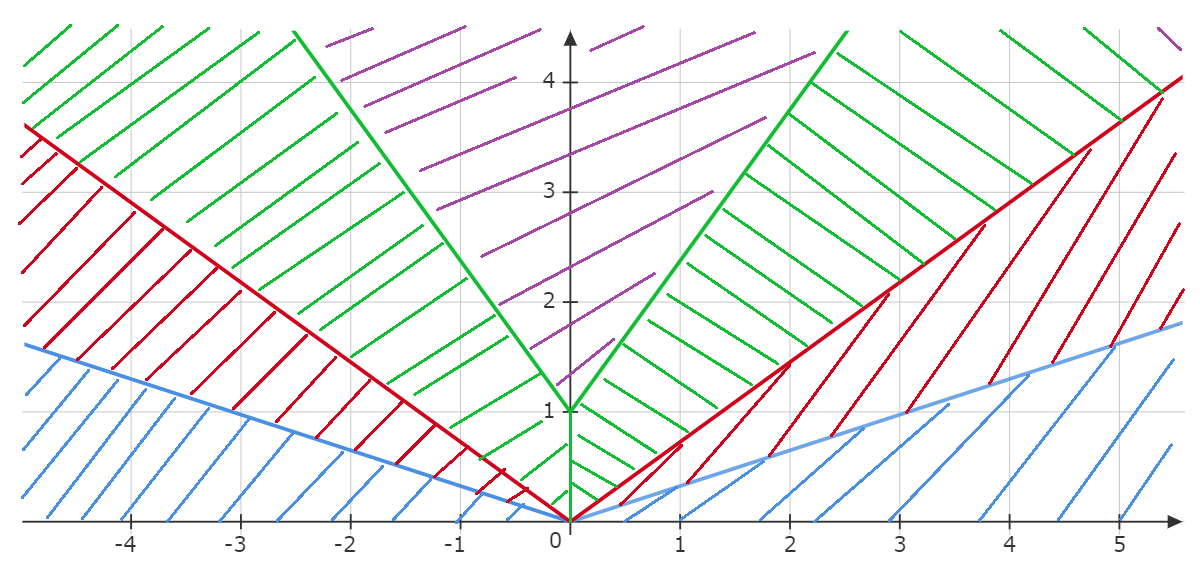
\includegraphics[width=0.5\textwidth]{Figures/AlphaFirstDecomposition.png}
	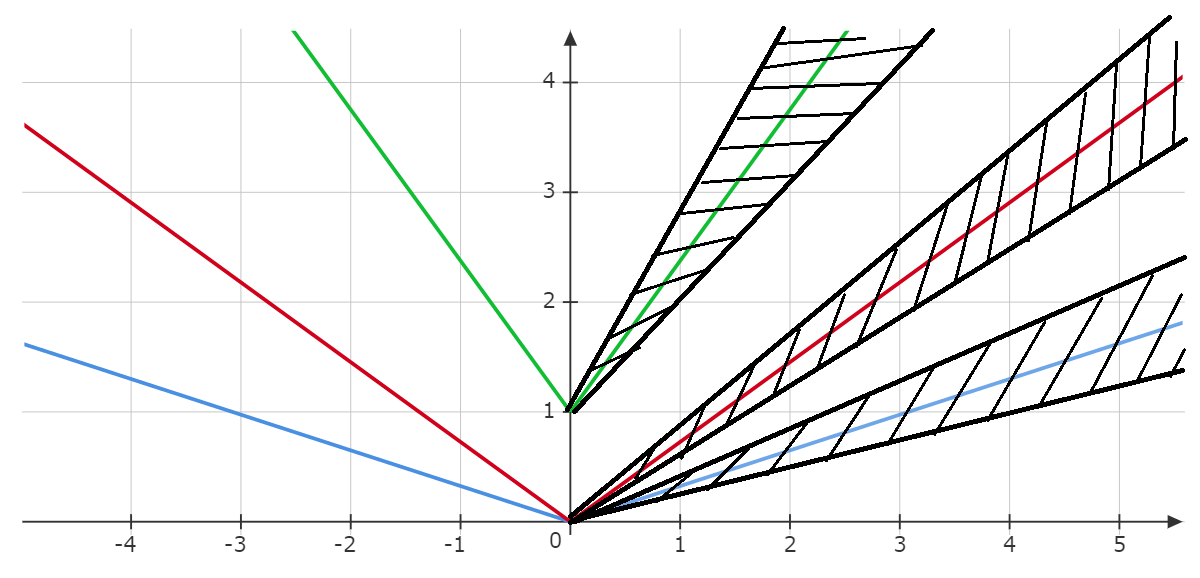
\includegraphics[width=0.5\textwidth]{Figures/AlphaSecondDecomposition.png}
	\caption{This figure shows the support of the different automorphisms present in the decomposition of an SQ$_1$-automorphism acting on the upper half plane.}
	\label{fig:SetupSQAut}
\end{figure}
 As a remark, notice that this definition is not exactly identical to de definition given in \cite{ogata2021h3gmathbb} due to the translation operators.
 \begin{definition}
 	Take $\alpha\in\Aut{\AA}$. We say that $\alpha\in\textrm{HAut}_1(\AA)$ if and only if for any $0<\theta<\pi/2$ there exists an $a\in\AA$ and some $\alpha_\sigma\in\Aut{\AA_{C_\theta}\cap\AA_\sigma}$ for each $\sigma\in\{L,R\}$ such that
 	\begin{equation}
 		\alpha=\Ad{a}\circ\alpha_L\otimes\alpha_R.
 	\end{equation}
 \end{definition}
We will need one additional class of automorphisms:
\begin{definition}
	Take $\alpha\in\Aut{\AA}$. We say that $\alpha\in\textrm{VAut}_1(\AA)$ if and only if there exists some $a\in\AA$, $\alpha_U\in\Aut{\tau(\AA_{C_\theta^c}\cap\AA_{U})}$ and an $\alpha_D\in\Aut{\tau^{-1}(\AA_{C_\theta^c}\cap\AA_{D})}$ such that
	\begin{equation}
		\alpha=\Ad{a}\circ\alpha_U\otimes\alpha_D.
	\end{equation}
	If furthermore $\alpha_U\circ\beta_g^U=\beta_g^U\circ\alpha_U$ we say that $\alpha\in\textrm{GVAut}_1(\AA)$.
\end{definition}
Now we will state some properties of locally generated automorphisms:
\begin{lemma}\label{lem:PropertiesLocallyGeneratedAutomorphisms}
	Take $H$ an interaction such that there exists a $0<\phi<1$ satisfying that $\norm{H}_{f_\phi}\leq 1$. The following statements now hold (for any $s,t\in\RR$):
	\begin{enumerate}
		\item $\gamma^H_{s;t}\circ\gamma^{H_D}_{t;s}\otimes\gamma^{H_U}_{t;s}\in\textrm{HAut}(\AA)$.
		\item $\gamma^H_{s;t}\circ\gamma^{H_L}_{t;s}\otimes\gamma^{H_R}_{t;s}\in\textrm{VAut}(\AA)$. If additionally $H$ is a $G$-invariant interaction we even have $\gamma^H_{s;t}\circ\gamma^{H_L}_{t;s}\otimes\gamma^{H_R}_{t;s}\in\textrm{GVQAut}(\AA)$.
		\item $\gamma^{H_U}_{s;t}\otimes\gamma^{H_D}_{s;t}\in\textrm{SQAut}(\AA)$. If additionally $H$ is a $G$-invariant interaction we even have $\gamma^{H_U}_{s;t}\otimes\gamma^{H_D}_{s;t}\in\textrm{GSQAut}(\AA)$.
		\item If $H$ is $G$-invariant then $\gamma^{H}_{t;s}\circ\beta_g^U\circ\gamma^{H}_{s;t}\circ(\beta_g^U)^{-1}\in\textrm{HAut}(\AA)$.
		\item $\gamma^{H}_{t;s}\in\textrm{SQAut}(\AA)$.
	\end{enumerate}
\end{lemma}
\begin{proof}
	Part 1 is done in Proposition 5.5 in \cite{ogata2021h3gmathbb} and part 4 follows trivially from Part 1. Except for the translation operators in my definition of the $\textrm{SQAut}(\AA)$, part 3 follows from Theorem 5.2 in \cite{ogata2021h3gmathbb}. To show part 3 we therefore have to show that Theorem 5.2 in \cite{ogata2021h3gmathbb} still holds if we replace $\mathcal{C}_0$ and $\mathcal{C}_1$ in the proof by
	\begin{align}
		\mathcal{C}_0&\defeq \left\{C_{[0,\theta_1],\sigma},C_{]\theta_1,\theta_2],\sigma,\rho},C_{]\theta_2,\theta_3],\sigma,\rho}\cup\tau^{\rho}(C_{]\theta_2,\theta_3],\sigma,\rho}),\tau^\rho(C_{]\theta_3,\pi/2],\rho})|\sigma=\{L,R\},\rho=\{U,D\}\right\}\\
		\mathcal{C}_1&\defeq\{C_{[\theta_{0.8},\theta_{1.2}]\cap\sigma\cap\tau},C_{[\theta_{1.8},\theta_{2.2}]\cap\sigma\cap\tau},\tau^\rho(C_{[\theta_{2.8},\theta_{3.2}]\cap\sigma\cap\rho})|\sigma=\{L,R\},\rho=\{U,D\}\}.
	\end{align}
	Take the $\Psi$ from this proof to be our $H$, take $\Psi^{(0)}$ to be $\sum_{C\in\mathcal{C}_0}H_{C}$ (with our new definition of $\mathcal{C}_0$) and take $\Psi^{(1)}\defeq \Psi-\Psi^{(0)}$. Now define $\Xi^{(s)}(Z,t)$ through
	\begin{equation}\label{eq:PropertiesLocallyGeneratedAutomorphismsProofDefinitionXi}
		\Xi^{(s)}(Z,t)\defeq\sum_{m=0}^\infty \sum_{\substack{X\subset Z,\\X(m)=Z}}\Delta_{X(m)}(\gamma^\Psi_{s;t}(\Psi^{(1)}(X;t)))
	\end{equation}
	with these new definitions of $\Psi^{(0)}$ and $\Psi^{(1)}$. We now want so show that for every $t$,
	\begin{equation}
		\sum_{Z\subset\ZZ^2}\left(\Xi^{(s)}(Z,t)-\sum_{C\in\mathcal{C}_1}\id_{Z\subset C}\Xi^{(s)}(Z,t)\right)
	\end{equation}
	is bounded. Following the arguments in equation (5.22) to (5.24) in \cite{ogata2021h3gmathbb} we still get that
	\begin{equation}
		\sum_{\substack{Z\subset\ZZ^2,\\\nexists C\in\mathcal{C}_1:Z\subset C}}\sup_{t\in[0,1]}\norm{\Xi^{(1)}(Z,t)}\leq \frac{8}{C_F}(e^{2I_F(\Psi)}-1)\sum_{\substack{C_1,C_2\in\mathcal{C}_0,\\ C_1\neq C_2}}M(C_1,C_2)
	\end{equation}
	where
	\begin{equation}
		M(C_1,C_2)\defeq \sum_{m\geq 0}\sum_{\substack{X:\\\forall C\in\mathcal{C}_1,X\cap((C^c)(m))\neq\emptyset,\\X\cap C_1\neq\emptyset,X\cap C_2\neq\emptyset}}\left(\sup_{t\in[0,1]}(\norm{\Psi^{(1)}(X;t)})\abs{X}G_F(m)\right)
	\end{equation}
	is now defined using the new $\mathcal{C}_1$. To bound these $M(C_1,C_2)$ we will (just like in \cite{ogata2021h3gmathbb}) differentiate between two cases. That is, the case where $C_1$ and $C_2$ are adjacent\footnote{We say that $C_1$ and $C_2$ are adjacent if and only if $\#(C_1(1)\cap C_2(1))=\infty$.} and the case where they are not. We begin with the latter. In this case we still have in complete analogy with the proof in \cite{ogata2021h3gmathbb} that
	\begin{align}
		M(C_1,C_2)\leq b_0(C_1,C_2) &\defeq \sum_{m\geq 0}\sum_{\substack{X:X\cap C_1\neq\emptyset,\\X\cap C_2\neq\emptyset}}\left(\sup_{t\in[0,1]}(\norm{\Psi^{(1)}(X;t)})\abs{X}G_F(m)\right)\\
		&\leq \norm{\Psi_1}_F\sum_{\substack{x\in C_1\\y\in C_2}}F(d(x,y))\sum_{m=0}^\infty G_F(m)<\infty.
	\end{align}
	\footnote{Here $\Psi_1$ is defined through $\Psi_1(X)=\abs{X}^1 \Psi(X)$.} What is now left to show is the case where $C_1$ and $C_2$ are adjacent. Take $\tilde{C}\in\mathcal{C}_1$ such that $C_1\cap\tilde{C}\neq\emptyset$ and $C_2\cap\tilde{C}\neq\emptyset$. Take $L_1=\partial\tilde{C}/C_2$\footnote{Here $\partial \tilde{C}$ means the boundary of $\tilde C$.} and $L_2=\partial\tilde{C}/C_1$. By following the same reasoning that led to equation (5.36) in \cite{ogata2021h3gmathbb} we get that
	\begin{align}
		M(C_1,C_2)\leq b_0(C_1,C_2/\tilde{C})+b_0(C_1/\tilde{C},C_2)+b_0(\tilde{C}\cap C_2,(C_1\cup C_2)^c)+b_1(C_1\cap\tilde{C},C_2\cap\tilde{C},L_1,L_2)
	\end{align}
	where
	\begin{align}
		b_1(C_1\cap\tilde{C},C_2\cap\tilde{C},L_1,L_2)&\defeq\sum_{m=0}^\infty \sum_{\substack{X\subset \tilde{C}:\\ X\cap C_1\cap\tilde{C}\neq\emptyset\\X\cap C_2\cap\tilde{C}\neq\emptyset\\ X\cap (\tilde{C}^c(m))\neq\emptyset}}\sup_{t\in[0,1]}\norm{\Psi(X;t)}\abs{X}G_F(m)\\
		&\leq \norm{\Psi_1}_F\sum_{m=0}^{\infty}G_F(m)\left(\sum_{\substack{x\in C_2\cap\tilde{C},\\y\in L_1(m)}}+\sum_{\substack{x\in C_1\cap\tilde{C},\\y\in L_2(m)}}\right)F(d(x,y))<\infty.
	\end{align}
	Since the remainder of the proof can remain unchanged from \cite{ogata2021h3gmathbb}, this concludes the proof of item 3. The proof of item 5 just follows from the fact that for any $\alpha_1\in\textrm{SQAut}(\AA)$ and for any $\alpha_2\in\textrm{HAut}(\AA)$ we have that $\alpha_2\circ\alpha_1\in\textrm{SQAut}(\AA)$. We now only need to comment on item 2. We must show that
	\begin{equation}
		(\gamma^H_{s;t}\circ\gamma^{H_L}_{t;s}\otimes\gamma^{H_R}_{t;s})^{-1}=\gamma^{H_L}_{s;t}\otimes\gamma^{H_R}_{s;t}\circ\gamma^H_{t;s}\in\textrm{GVAut}(\AA).
	\end{equation}
	The proof of this starts analogously to the proof of item 1 and 3. We take $\Psi=H$, $\Psi^{(0)}=H_{\tau(C_\theta^c\cap U)}+H_{\tau^{-1}(C_\theta^c\cap D)}$ and $\Psi^{(1)}=\Psi-\Psi^{(0)}$. Define $\Xi^{(s)}(Z;t)$ again through equation \eqref{eq:PropertiesLocallyGeneratedAutomorphismsProofDefinitionXi}. In analogy to what was done in equation (5.54) in \cite{ogata2021h3gmathbb} we obtain
	\begin{equation}
		\sum_{\substack{Z:Z\nsubseteq \tau(C_\theta^c\cap U)\\\text{and }Z\nsubseteq \tau^{-1}(C_\theta^c\cap D)}}\sup_{t\in[0,1]}\norm{\Xi^{(1)}(Z,t)}\leq \frac{8}{C_F}(e^{2I_F(\Psi)}-1)\sum_{m=0}^\infty\sum_{\substack{X:X(m)\nsubseteq \tau(C_\theta^c\cap U)\\\text{and }X(m)\nsubseteq \tau^{-1}(C_\theta^c\cap D)}} \sup_{t\in[0,1]}\norm{\Psi^{(1)}(X;t)}\abs{X}G_F(m).
	\end{equation}
	If $X$ in the last line has a non-zero contribution, then at least one of the following occurs:
	\begin{enumerate}
		\item $X\cap (W(C_\theta)\cap L)\neq\emptyset$ and $X\cap R\neq\emptyset$.
		\item $X\cap (W(C_\theta)\cap R)\neq\emptyset$ and $X\cap L\neq\emptyset$.
		\item $X\subset W(C_\theta)^c$ and
		\begin{enumerate}
			\item $X\subset U,X\subset D$, or
			\item $X\subset U,X\subset L,X\subset R$ and $X(m)\cap (\tau^{-1}(C_\theta^c\cap D))^c\neq \emptyset$, or
			\item $X\subset D,X\subset L,X\subset R$ and $X(m)\cap (\tau(C_\theta^c\cap U))^c\neq \emptyset$.
		\end{enumerate}
	\end{enumerate}
	This shows that we have a bound
	\begin{align}
		&\sum_{\substack{Z:Z\nsubseteq \tau(C_\theta^c\cap U)\\\text{and }Z\nsubseteq \tau^{-1}(C_\theta^c\cap D)}}\sup_{t\in[0,1]}\norm{\Xi^{(1)}(Z,t)}\\
		\nonumber
		&\leq \frac{8}{C_F}(e^{2I_F(\Psi)}-1)(b_0(W(C_\theta)\cap L,R)+b_0(L,W(C_\theta)\cap R)+b_0(W(C_\theta)^c\cap U,W(C_\theta)^c\cap D)\\
		\nonumber
		&\qquad+b_1(W(C_\theta)^c\cap U\cap L,W(C_\theta)^c\cap U\cap L,L\cap\partial(W(C_\theta)^c\cap U),R\cap\partial(W(C_\theta)^c\cap U))\\
		&\qquad b_1(W(C_\theta)^c\cap D\cap L,W(C_\theta)^c\cap D\cap R,L\cap\partial(W(C_\theta)^c\cap D),R\cap\partial(W(C_\theta)^c\cap D)))<\infty.
	\end{align}
	This concludes the proof.
\end{proof}
This implies certain things for our locally generated automorphisms.
From these four statements we can prove the following results:
\begin{lemma}\label{lem:TwoAngleLemmaPart1}
	Take $\theta_1$ and $\theta_2$ such that $0<\theta_1<\theta_2<\pi/2$ then for all $\Theta\in\Aut{\AA_{W(C_{\theta_2})^c}}$ and $s,t\in\RR$ there exists an $a_1\in\UU(\AA)$ and a $\tilde{\Theta}\in \Aut{\AA_{W(C_{\theta_1})^c}}$ such that
		\begin{equation}\label{eq:TwoAngleLemmaPart1Equation1}
			\gamma^{H}_{t;s}\circ\Theta\circ\gamma^{H}_{s;t}=\Ad{a_1}\circ\tilde{\Theta}.
		\end{equation}
\end{lemma}
\begin{proof}
	We have that
	\begin{equation}
		\gamma^{H}_{t;s}\circ\Theta\circ\gamma^{H}_{s;t}=\gamma^{H_D}_{t;s}\otimes\gamma^{H_U}_{t;s}\circ\gamma^{H_D}_{s;t}\otimes\gamma^{H_U}_{s;t}\circ\gamma^{H}_{t;s}\circ\Theta\circ\gamma^{H}_{s;t}\circ\gamma^{H_D}_{t;s}\otimes\gamma^{H_U}_{t;s}\circ\gamma^{H_D}_{s;t}\otimes\gamma^{H_U}_{s;t}.
	\end{equation}
	Using that $\gamma^{H}_{s;t}\circ\gamma^{H_D}_{t;s}\otimes\gamma^{H_U}_{t;s}\in\textrm{HAut}_1(\AA)$ we get that there exists some $a\in\AA$ and $\eta\in\Aut{\AA_{C_\theta}}$ such that
	\begin{align}
		\gamma^{H}_{t;s}\circ\Theta\circ\gamma^{H}_{s;t}&=\Ad{a}\circ \gamma^{H_D}_{t;s}\otimes\gamma^{H_U}_{t;s}\circ\eta_{s;t}^{-1}\circ\Theta\circ\eta_{s;t}\circ\gamma^{H_D}_{s;t}\otimes\gamma^{H_U}_{s;t}\\
		&=\Ad{a}\circ \gamma^{H_D}_{t;s}\otimes\gamma^{H_U}_{t;s}\circ\Theta\circ\gamma^{H_D}_{s;t}\otimes\gamma^{H_U}_{s;t}.
	\end{align}
	Since by \ref{lem:PropertiesLocallyGeneratedAutomorphisms} part 3 $\gamma^{H_D}_{s;t}\otimes\gamma^{H_U}_{s;t}\in\textrm{GSQAut}(\AA)$ the result follows.
\end{proof}
\begin{lemma}\label{lem:TwoAngleLemmaPart2}
	Take $\theta_1$ and $\theta_2$ such that $0<\theta_1<\theta_2<\pi/2$. Then for all $\eta_{g}^{\sigma}\in\Aut{\AA_{C_{\theta_1}}\cap\AA_{\sigma}}$ (where $\sigma\in\{L,R\}$ and $g\in G$) and $s,t\in\RR$ there exist $a_{2},\in\UU(\AA),a_{3,\sigma}\in\UU(\AA_\sigma)$ and some $\tilde{\eta}_{\sigma}^g\in \Aut{\AA_{C_{\theta_2}}\cap\AA_{\sigma}}$ such that
	\begin{align}
		\label{eq:TwoAngleLemmaPart2Equation1}
		\gamma^{H}_{t;s}\circ\eta_{g}^L\otimes\eta_{g}^R\circ\gamma^{H}_{s;t}&=\Ad{a_2}\circ(\tilde\eta_{g}^L \otimes\tilde\eta_{g}^R)\\
		\label{eq:TwoAngleLemmaPart2Equation2}
		\gamma^{H_\sigma}_{t;s}\eta_g^\sigma\gamma^{H_\sigma}_{s;t}&=\Ad{a_{3,\sigma}}\circ \tilde\eta_{g}^\sigma.
	\end{align}
\end{lemma}
\begin{proof}
	First we show that equation \eqref{eq:TwoAngleLemmaPart2Equation2} implies equation \eqref{eq:TwoAngleLemmaPart2Equation1}. This is because using equation \eqref{eq:TwoAngleLemmaPart2Equation1} we get that
	\begin{align}
		\gamma^H_{t;s}\circ\eta_g\circ\gamma^{H}_{s;t}&=\gamma^H_{t;s}\circ\gamma^{H_L}_{s;t}\otimes\gamma^{H_R}_{s;t}\circ\gamma^{H_L}_{t;s}\otimes\gamma^{H_R}_{t;s}\circ\eta_g\circ\gamma^{H_L}_{s;t}\otimes\gamma^{H_R}_{s;t}\circ\gamma^{H_L}_{t;s}\otimes\gamma^{H_R}_{t;s}\circ\gamma^H_{s;t}\\
		&=\gamma^H_{t;s}\circ\gamma^{H_L}_{s;t}\otimes\gamma^{H_R}_{s;t}\circ\Ad{a_{3,L}\otimes a_{3,R}}\circ\tilde{\eta}_g\circ\gamma^{H_L}_{t;s}\otimes\gamma^{H_R}_{t;s}\circ\gamma^H_{s;t}.
	\end{align}
	If one now uses the fact that $\gamma^H_{t;s}\circ\gamma^{H_L}_{s;t}\otimes\gamma^{H_R}_{s;t}\in\textrm{GVAut}_1(\AA)$ the implication follows. To finish the proof we now only have to use the fact that the $\gamma^{H_\sigma}_{0;1}$ are in $\textrm{SQAut}_1(\AA)$.
\end{proof}
\subsection{The two translation symmetries}
 This section will define the classes of automorphisms required in the assumptions and proofs about the $H^1$-valued translation index. In analogy with section 2.1 from \cite{ogata2021h3gmathbb} we will define some classes of automorphisms (see figure \ref{fig:SetupSQAut2}):
\begin{definition}
	Take $\alpha\in\Aut{\AA}$. We say that $\alpha\in\textrm{SQAut}_2(\AA)$ if and only if for any $0<\theta_{0.8}<\theta_{1}<\theta_{1.2}<\theta_{1.8}<\theta_{2}<\theta_{2.2}<\theta_{2.8}<\theta_3<\theta_{3.2}<\pi/2$ there exist $a\in\AA$, $\alpha_{[0,\theta_1], \sigma}\in\Aut{\AA_{C_{[0,\theta_1]}\cap\sigma}},\:\alpha_{]\theta_1,\theta_2],\sigma,\rho}\in\Aut{\AA_{C_{]\theta_1,\theta_2]}\cap\rho\cap\sigma}},\:\alpha_{]\theta_2,\theta_3],\sigma,\rho}\in\Aut{\AA_{(C_{]\theta_2,\theta_3]}\cap\rho\cap\sigma)\cup\tau^{\rho}(C_{]\theta_2,\theta_3]}\cap\rho\cap\sigma)}},\alpha_{]\theta_3,\pi/2],\rho}\in\Aut{\tau^\rho(\AA_{C_{[\theta_3,\pi/2]}\cap\rho})},\:\alpha_{]\theta_{0.8},\theta_{1.2}],\sigma,\rho}\in\Aut{\AA_{C_{]\theta_{0.8},\theta_{1.2}]}\cap\rho\cap\sigma}},\:\alpha_{]\theta_{1.8},\theta_{2.2}],\sigma,\rho}\in\Aut{\AA_{C_{]\theta_{1.8},\theta_{2.2}]}\cap\rho\cap\sigma}}$ and  $\alpha_{]\theta_{2.8},\theta_{3.2}],\sigma,\rho}\in\Aut{\tau^{\rho}(\AA_{C_{]\theta_{2.8},\theta_{3.2}]}\cap\rho\cap\sigma})}$ for any $\rho\in\{U,D\}$ and $\sigma\in\{L,R\}$ (here $\tau^U=\tau$ and $\tau^D=\tau^{-1}$) such that
	\begin{equation}
		\alpha=\Ad{a}\circ \bigotimes_{\sigma}\alpha_{[0,\theta_1],\sigma}\circ\bigotimes_{\sigma,\rho}\alpha_{]\theta_1,\theta_2],\sigma,\rho}\circ\bigotimes_{\rho}\alpha_{[\theta_3,\pi/2]}\circ\bigotimes_{\rho,\sigma}\left(\alpha_{]\theta_{0.8},\theta_{1.2}],\rho,\sigma}\otimes\alpha_{]\theta_{1.8},\theta_{2.2}],\rho,\sigma}\otimes\alpha_{]\theta_{2.8},\theta_{3.2}],\rho,\sigma} \right).
	\end{equation}
	If additionally everything (except $a$) commutes with $\beta_g^U$ we say that $\alpha\in \textrm{GSQAut}_2(\AA)$.
\end{definition}
\begin{figure}
	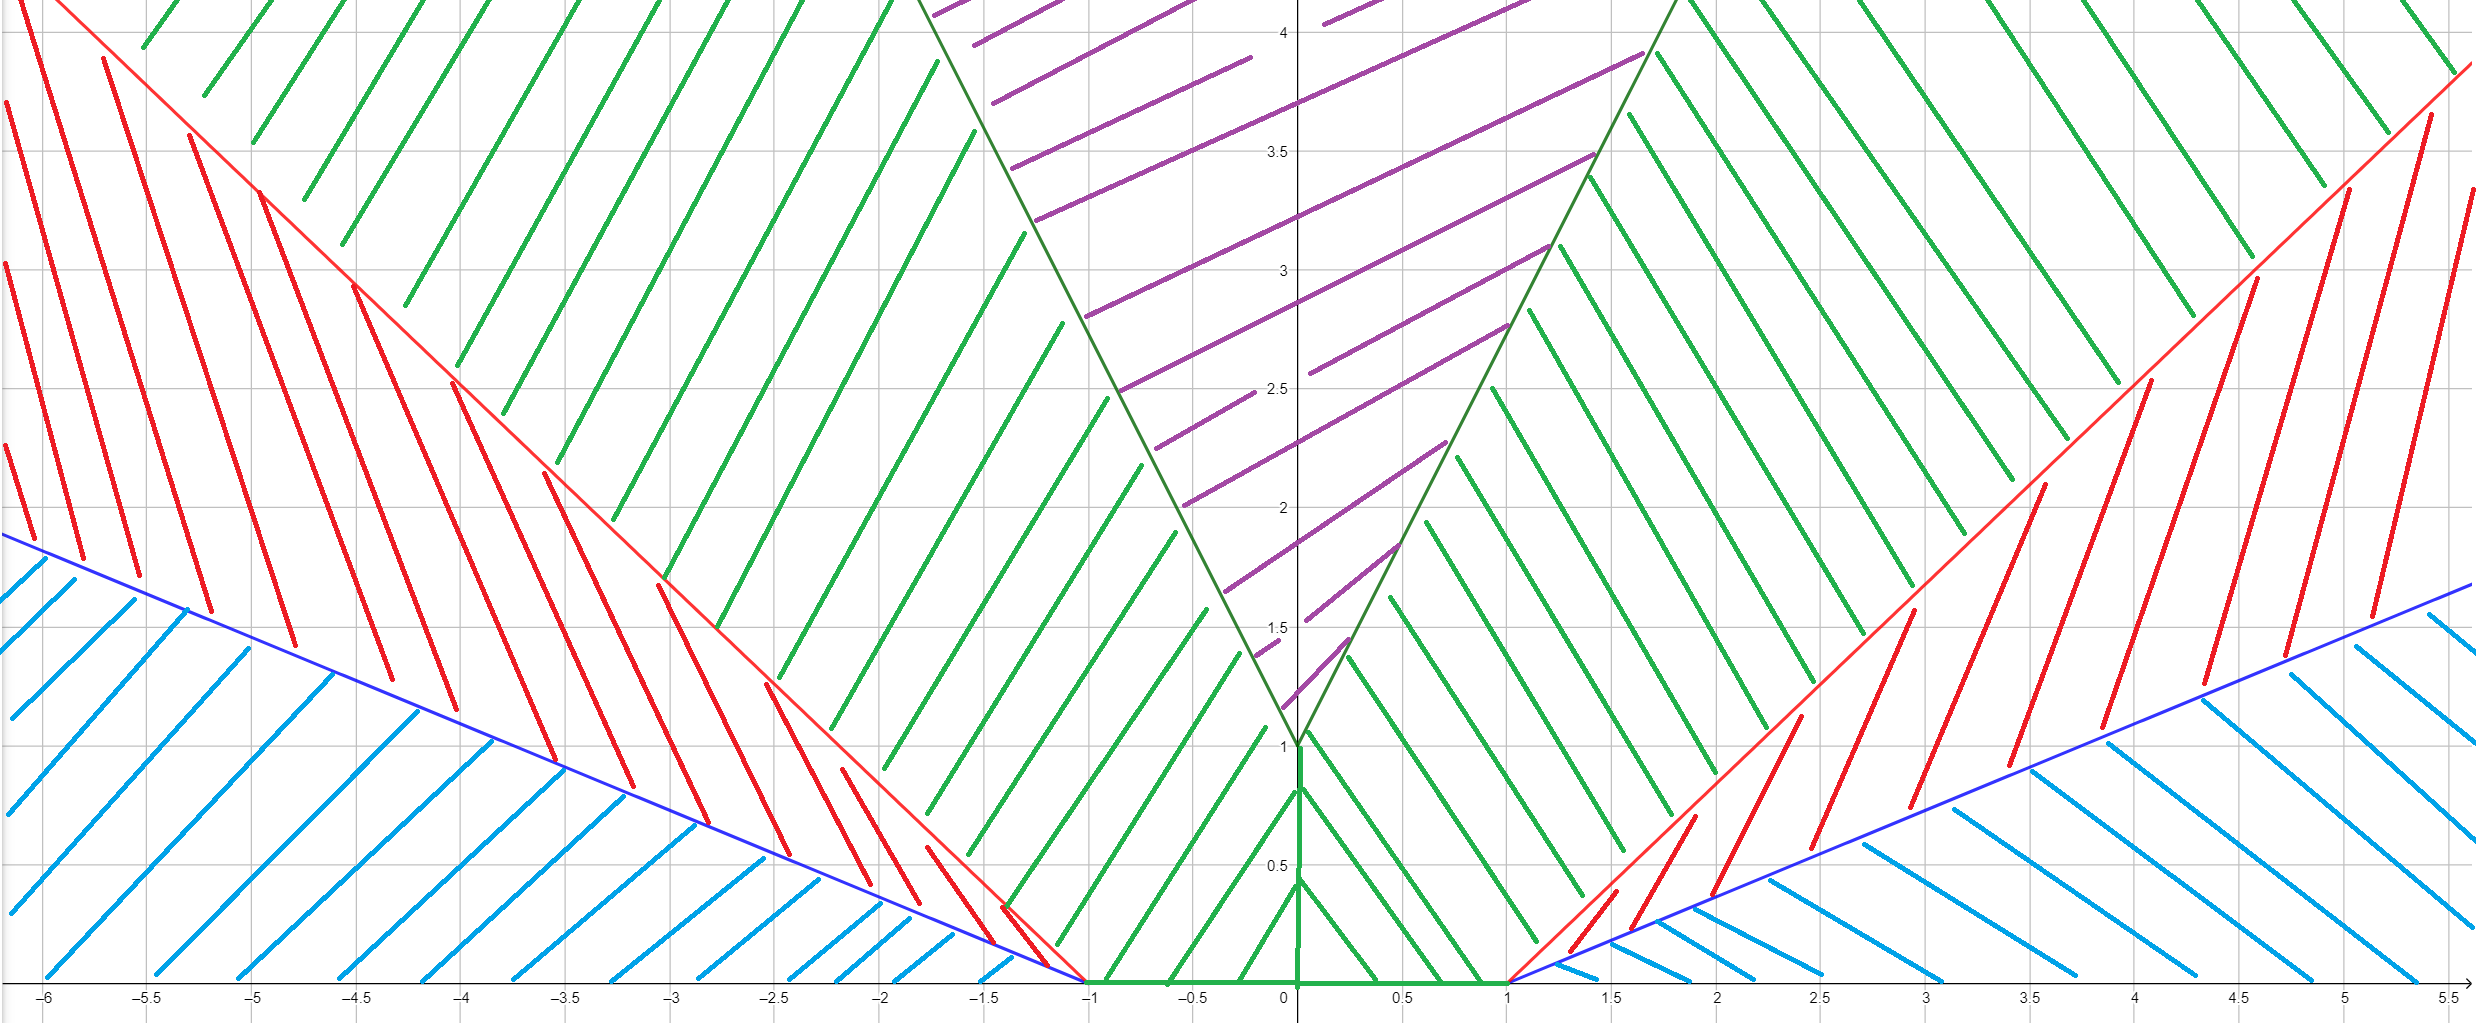
\includegraphics[width=0.5\textwidth]{Figures/AlphaFirstDecomposition2.png}
	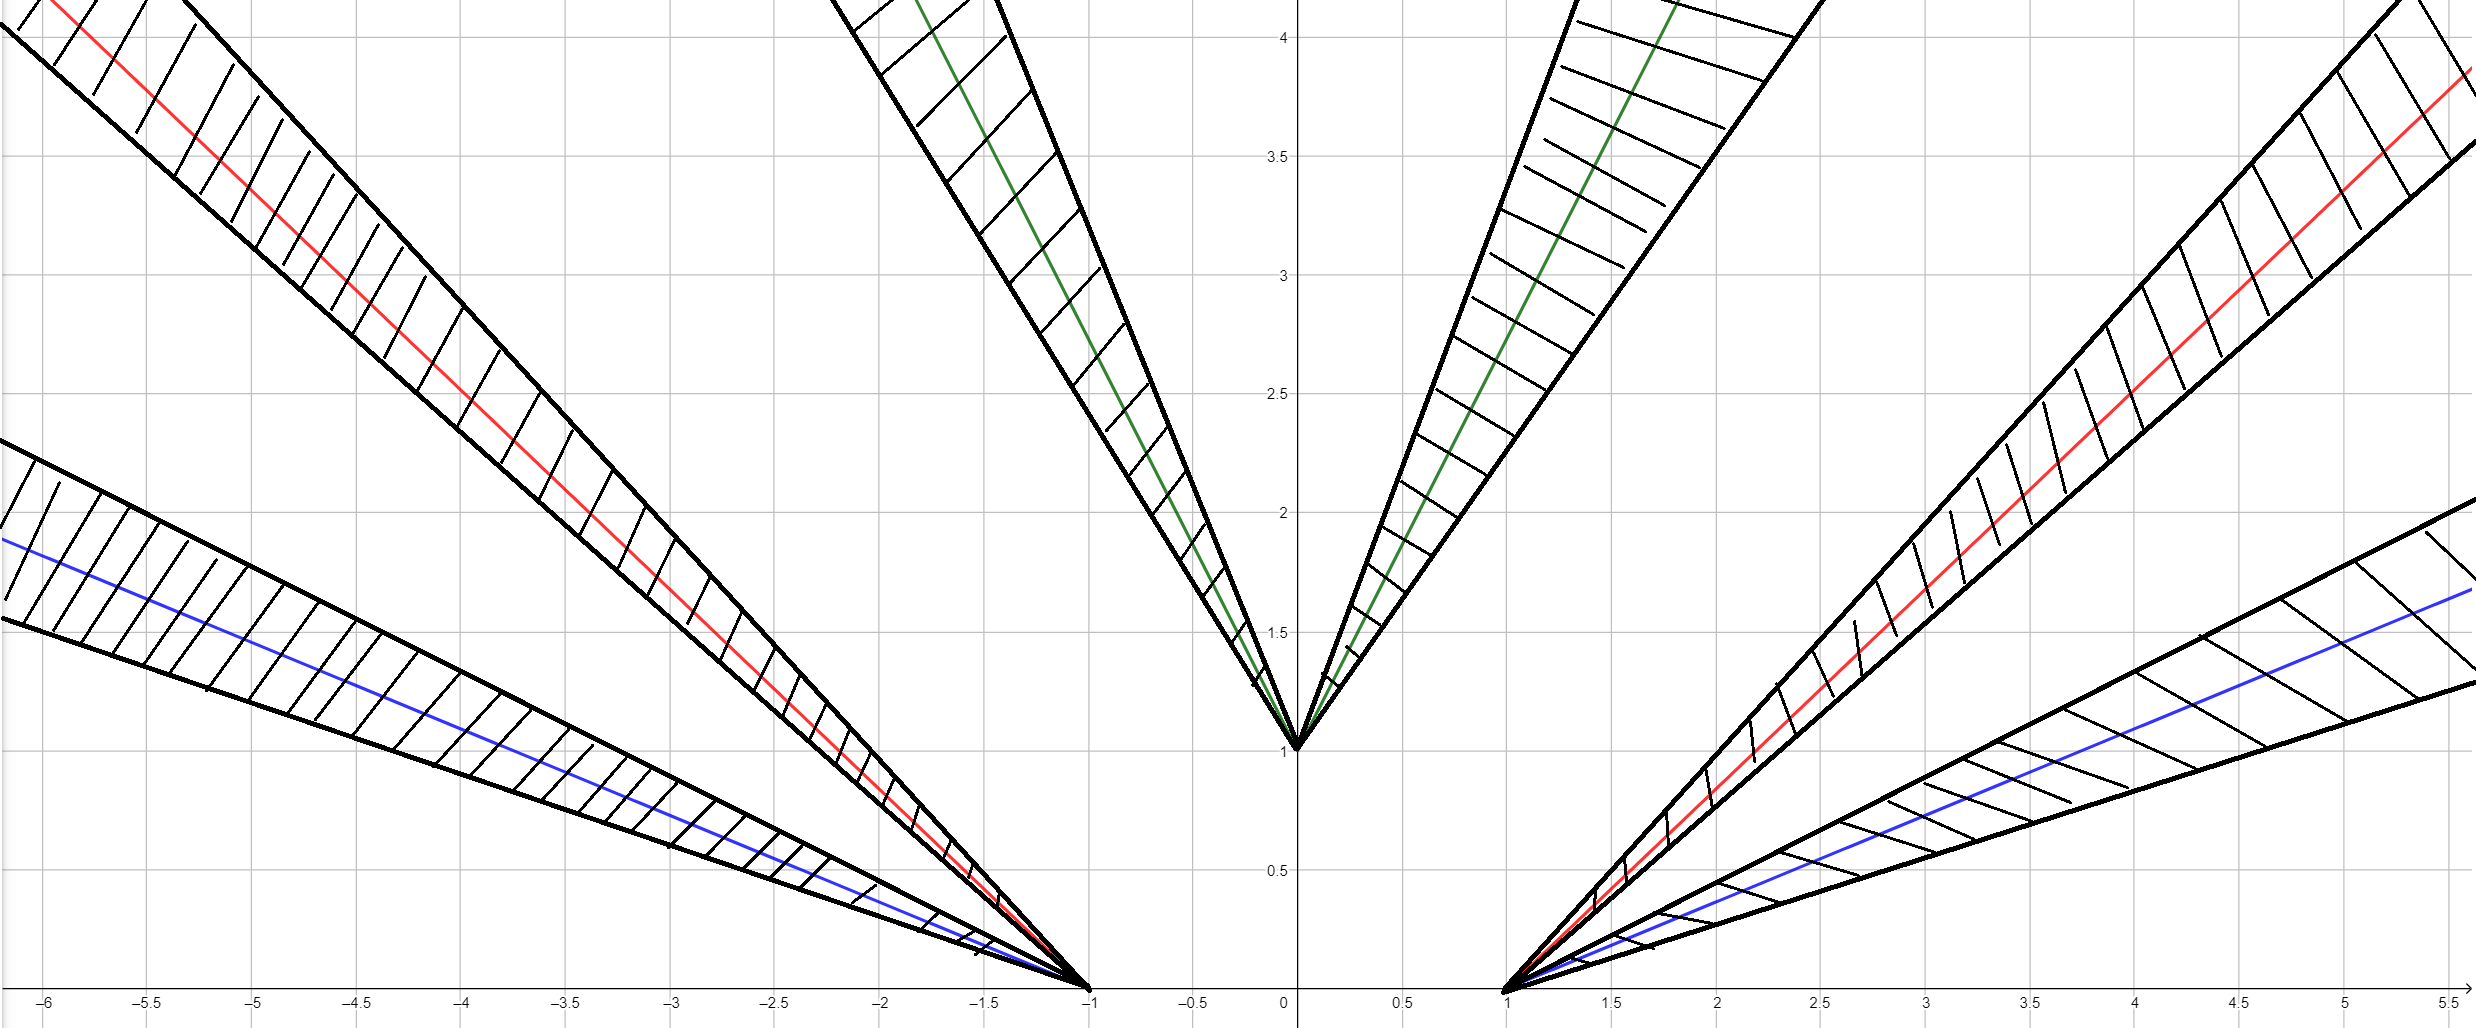
\includegraphics[width=0.5\textwidth]{Figures/AlphaSecondDecomposition2.png}
	\caption{This figure shows the support of the different automorphisms present in the decomposition of an SQ$_2$-automorphism acting on the upper half plane.}
	\label{fig:SetupSQAut2}
\end{figure}
\bibliography{TSPT}
\bibliographystyle{plain}
\end{document}